\documentclass[a4paper]{article} 
\usepackage[longend,ruled,linesnumbered]{algorithm2e}
\input{head}
\usetikzlibrary{arrows,shapes,automata,petri}
\tcbuselibrary{theorems}
\usepackage{caption}
\usepackage{subcaption}
\newtcbtheorem[]{teorema}{}%
{colback=gray!15,colframe=gray!70}{th}

\begin{document}
%-------------------------------
%	TITLE SECTION
%-------------------------------

\fancyhead[C]{}
\hrule \medskip % Upper rule
\begin{minipage}{0.295\textwidth} 
\raggedright
\footnotesize
Andrei Gabriel Taraboi \hfill\\   
@conerns\hfill\\
\end{minipage}
\begin{minipage}{0.4\textwidth} 
\centering 
\large 
Modelli della concorrenza\\ 
\normalsize 
\end{minipage}
\begin{minipage}{0.295\textwidth} 
\raggedleft
\hfill\\
\end{minipage}
\medskip\hrule 
\bigskip

%-------------------------------
%	CONTENTS
%-------------------------------
\tableofcontents
\newpage
\section{Lezione del 5 ottobre}

La concorrenza è una caratteristica dei sistemi di elaborazione nei quali può verificarsi
che un insieme di processi o sotto-processi(thread) computazionali sia in esecuzione nello
stesso istante. 

Per i programmi che presentano concorrenza al loro interno possimao definire delle caratteristiche generali.
\begin{itemize}
    \item Competizione per l'accesso alle risorse condivise
    \item Cooperazione per un fine comune
    \item Coordinamento di attività diverse
    \item Sincronia/Asincoria 
\end{itemize}
%------------------------------------------------

\subsection{Logica proposizionale}
\subsubsection{Sintassi}
Definiamo la sintassi: \hfill \newline
$\mathbf{P} = \{p_1,p_2 \dots, p_i\}$, sono i nostri simboli preposizionali (infiniti ma numerabili) \hfill \newline
$\bot$ e $\top$ sono invece le nostre costanti logiche (anche atomiche) \hfill \newline
$\neg, \ \lor, \ \land , \ \to, \ \Leftrightarrow$ rappresentano i nostri connettivi logici, attraverso loro possiamo creare delle formule ben formate. \hfill \newline
$( \,,) $ sono invece i delimitatori delle componenti atomiche oppure delle formule ben formate.
\bigskip

Vogliamo definire l'insieme delle formule ben formate $F_{Prop}$. L'insieme viene definito in modo induttivo:
\begin{enumerate}
    \item $\top, \bot, p_i \in F_{Prop}$
    \item $A \in F_{Prop},  B \in F_{Prop}$: ovvero siano A e B delle formule ben formate, possiamo allora dire che:
    \begin{itemize}
        \item $(\neg A), (A \lor B), (A \land B), (A \to B), (A \Leftrightarrow B) \in F_{Prop}$, ovvero che unendo le due formule ben formate attraverso dei connettivi logici, il risultato corrisponde a delle formule ben formate. 
    \end{itemize}
\end{enumerate}

\subsubsection{Semantica}
La semantica di una formula è il suo valore di verità, ovvero il fatto che sia vera o falsa. 

Sia $V: P \to \{0, 1\}$ una assegnazione booleana che assegna ad ogni proposizione atomica un valore di verità. Questa assegnazione, in maniera induttiva, si estende alle formule:

Sia $I_v(p_i) = V(p_i), I_v(\top) = 1, I_v(\bot) = 0$, dobbiamo ora definire per ogni forma composta definita, come queste formano il valore di verità della formula composta.
\begin{itemize}
    \item $I_v(\neg A) = 1 - I_v(A)$ (negazione del valore ottenuto)
    \item $I_v(A \lor B) = I_v(A) \lor I_v(B)$
    \item $I_v(A \land B) = I_v(A) \land I_v(B)$
    \item $I_v(A \to B) = I_v(\neg A) \lor I_v(B)$
    \item $I_v(A \Leftrightarrow B) = I_v(\neg A \lor B) \land I_v(\neg B \lor A)$ (qui si potrebbe andare avanti)
\end{itemize}

\section{Lezione del 7 ottobre}
%------------------------------------------------
Come facciamo a determinare se l'output di un determinato programma è corretto?
\newline 
\begin{algorithm}[H]
    \SetAlgoLined
    int x = v[0]; \textit{x è il massimo in $v[0, \dots, 0]$} \\
    int h = 1; \textit{ora x è il massimo in $v[0, \dots, h-1]$}\\
    
    \While{h $<$ n}{ \textit{x è il massimo in $v[0, \dots, h-1]$ questo lo suppongo} \\
        \lIf{x $<$ v[h]}
        {
            x = v[h] \textit{x è il massimo in $v[0, \dots, h]$}
        } 
        h = h + 1; \textit{x è il massimo in $v[0, \dots, h-1], h \leq n$}
    }
    \textit{x è il massimo in $v[0, \dots, h-1], h = n$} \\
    \Return x;
    \caption{int f(int n, const int v[])}
\end{algorithm}

L'algoritmo restituisce il valore massimo presente all'interno del vettore v. Suppongo che n sia un numero positivo $n > 0$, e che un elemento generico del vettore sia un intero $v[i] \in \mathbb{Z}$ per i $\in \{0, \dots, n-1\}$. 
\hfill \newline \newline 
Dal momento che la proprietà \textit{x è il massimo in $v[0, \dots, h-1]$} è vera all’inizio dell’iterazione, ovvero nella riga 4 del codice, alla fine del codice nella riga 8, e prima dell’iterazione stessa presente alla riga 2, per induzione si può concludere che qualunque sia il numero di iterazioni che vengono svolte, la proprietà \textit{x è il massimo in $v[0, \dots, h-1]$} è invariante.
\newline\newline
Precondizione :  $\forall i \in  \{0, \dots, n-1\}, v[i] \in \mathbb{Z}$ e supponiamo inoltre che $n > 0$. \newline
Postcondizione : $\forall i \in  \{0, \dots, n-1\}, \ v[i] \leq x$ \newline
\hspace*{2.5cm} $\exists i \in \{0, \dots, n - 1\}, v[i] = x$ \newline
Le post condizioni indicate, insieme, ci conducono a dire che $x = max(v[0, \dots, n-1)$

La precondizione esprime ciò che vale all'inizio o più esattamente ciò che supponiamo valga a inizio esecuzione, la postcondizione è ciò che vale alla fine dell'esecuzione.
\newline 

Possiamo definire lo stato della memoria (s) come una funzione che va dall'insieme delle variabili del programma (V) un valore. $s : V \to \mathbb{Z}$

Data una formula $\phi$ e uno stato $s$, possiamo verificare se la formula è vera/valida/verificata in $s$. Una particolare formula che gode della proprietà di essere invariante, se è vera all’inizio di un’iterazione, allora è vera anche alla fine dell’iterazione.

Quando si esegue una istruzione, in genere, essa cambia lo stato della memoria. Scrivendo un programma risulta considerabile come un trasformatore di stato, perché le istruzioni che esegue generano un cambio dello stato della memoria. Un programma che non termina non ha stato uno stato finale, e quanto detto prima non è più valido in questo caso specifico.

Possiamo esprimere la nostra specifica di correttezza di un programma attraverso una tripla: $\alpha,P, \beta $. Dove $\alpha,\beta $ sono le nostre formule della logica proposizionale e $P$ è un programma(o fragmento di codice). Inoltre $\alpha$ è la nostra formula di precondizione e $\beta$ è la nostra formula di postcondizione.

\subsection{Logica di Hoare}
Le formule nella logica di Hoare sono triple che si presentano nella seguente forma: $\alpha,P, \beta$.

Abbiamo un linguaggio e un elemento fondamentale all'interno di questo linguaggio è il\textit{comando} C.
\textit{C::} $x := E$, con: 
\begin{itemize}
    \item x identificatore della variabile 
    \item := simbolo per l'assegnamento 
    \item E simbolo non terminale della grammatica che sta per \textit{espressione}
\end{itemize}
Quando abbiamo delle espressioni semplici possiamo combinarle in diversi modi:
\begin{itemize}
    \item in sequenza, aggiungendo un \textit{;} tra i due comandi: C ; C
    \item istruzione di scelta, if B then C else C endif
    \begin{itemize}
        \item B è un'espressione booleana, un simbolo non terminale della grammatica che dobbiamo poi in seguito definire.
    \end{itemize}
    \item istruzione iterativa, while B do C endwhile
    \item SKIP, un'istruzione fittizia semplicemente avanza il program counter ma non fa nulla
\end{itemize}

B:= true $|$ false $|$ not B $|$ B AND B $|$ B OR B $|$ E $<$ E $|$ E $>$ E $|$ E $=$ E
\begin{itemize}
    \item true e false sono costanti booleani (non sono delle formule logiche ma elementi del linguaggio)
    \item E espressioni aritmetiche costruite con nomi di variabili ed eventualmente costanti numeriche
\end{itemize}

\subsubsection{Esempio di programma}
\begin{algorithm}[H]
    \SetAlgoLined
    x := a; y := b; \\
    \While{x $!=$ y}{ 
        \lIf{x $<$ y}{ y := y - x}
        \Else{ x: = x - y;}
    }
    \caption{Programma D}
\end{algorithm}

Questo programma soddisfa la tripla $\{a> 0 \land b > 0\}$ D $\{x = MCD(a,b)\}$?

Come va letta la tripla nella logica di Hoare? Se si esegue il programma D a partire da uno stato della memoria in cui i valori di a sono maggiori di 0 e b è maggiore di zero allora alla fine dell'esecuzione il valore di x  sarà il massimo comune divisore tra a e b.

\subsubsection{Dimostrazione}
Una dimostrazione in una logica data è una sequenza di assiomi o formule derivate di quella
logica. \begin{itemize}
    \item assiomi, sono formule supposte vere a priori.
    \item formule derivate,  formule che derivano da altre formule precedenti applicando una regola di derivazione o di inferenza.
\end{itemize}
Una regola di derivazione ha la forma:
$$\displaystyle \frac{\alpha_1, \alpha_2, \dots \alpha_k}{\alpha}$$ 
\begin{itemize}
    \item $\alpha_1, \alpha_2, \dots \alpha_k$  premesse, formule che sono già state derivate o assiomi
    \item $\alpha$ conclusione, nuova formula
\end{itemize}
In questo caso ognuna delle $\alpha_i$, inclusa $\alpha$ la nostra conclusione,  è una formula tripla della logica di Hoare.
Quindi una dimostrazione si ottiene applicando ripetutamente le regole di derivazione fino ad
arrivare alla conclusione.

\subsubsection{Regole di derivazione}
\begin{enumerate}
    \item \textit{skip}, dal momento che non fa nulla, non cambia lo stato della memoria e quindi non occorrono premesse. Possiamo derivare quindi una tripla dove la pre e la post condizione coincidono
    $\displaystyle \frac{}{\{p\}skip\{p\}}$
    \item regola di conseguenza o implicazione, ci sono due premesse. 
    \begin{itemize}
        \item Una non è una tripla di Hoare ma è una implicazione nella logica preposizionale.
        $p \to p'$
        \item La seconda è una tripla di Hoare nella forma $\{p'\}C\{q\}$. 
    \end{itemize} 
    Ritrovandoci quindi a dover scrivere: $\displaystyle \frac{p \to p' ,\ \{p'\}C\{q\}}{\{p\} C \{q\}}$, questa regola ha una forma speculare: \\ $\displaystyle \frac{\{p\}C\{q'\} ,\ q' \to q }{\{p\} C \{q\}}$
    \item struttura di sequenza dei programmi: abbiamo due premesse $\displaystyle \frac{\{p\}C_1\{q\} \quad \{q\}C_2\{r\}}{\{p\}C_1,C_2\{r\}}$
    \item regola di assegnamento: Questa regola ha uno status particolare essendo l'unica regola che non ha premesse. 
    $\displaystyle \frac{}{\{p[E/x]\}x := E\{p\}}$ 
    \begin{itemize}
        \item \textit{p} è la formula che generalmente contiene gli identificatori delle variabili del programma
        \item \textit{$\{p[E/x]\}$} è formula nella quale l’espressione sostituisce tutte le occorrenze della variabile $x$.
        \item \textit{$[E/x]$} indica invece una sostituzione
    \end{itemize}
\end{enumerate}
\section{Lezione del 12 ottobre}
\subsection{Logica di Hoare}

\begin{itemize}
    \item \textbf{Istruzioni di scelta}: L'istruzione di     scelta fa parte delle regole di derivazione viste     nella lezione precedente. 

    L'istruzione si presenta nella forma: $\{p\} \textbf{if} \ B \ \textbf{then} \ C \ \textbf{else} \ D \ \textbf{endif} \{q\}$.
    
    
    Cerchiamo premesse che permettono di derivare questa istruzione. Nella situazione attuale la condizione che possiamo eseguire può essere o \textit{C} o \textit{D}. Valutiamo separatamente le due possibilità:
    \begin{itemize}
        \item Nel caso in cui la condizione del \textbf{if} fosse vera: $\{p \land B\}$ C $\{q\}$ 
            \item All'inizio dell'esecuzione è falsa la condizione \textit{B}, in questo caso: $\{p \land \neg B\}$ D $\{q\}$ 
        \end{itemize}
        Entrambe queste due triple sono delle premesse dalle quali possiamo dedurre la tripla risultante, ricaviamo quindi la formula generale della regola di derivazione
            $\displaystyle \frac{
                    \{p \land B \} C \{q\} \ \{p \land \neg B\} D \{q\}
                }
                {
                    \{p\} \textbf{if} \ B \ \textbf{then} \ C \ \textbf{else} \ D \ \textbf{endif} \{q\}
                }$
                
    \item \textbf{Istruzioni interattive} si presentano nella forma $\textbf{while} \ B \ \textbf{do} \ c \ \textbf{endwhile}$ che chiameremo $W$ successivamente
    abbiamo quindi la seguente tripla.
    $\{p \} W \{q\}$  Se eseguo il comando W a partire dallo stato in cui vale p, alla fine deve valere q.
    
    \begin{itemize}
        \item correttezza parziale, supponiamo a priori che l'esecuzione termini, senza dimostrarlo. Lo supponiamo solamente. La tripla ci darà solamente una soluzione parziale.
        \item si deve dimostrare che l'esecuzione termini. Si procede quindi prima dimostrando la correttezza parziale aggiungendo poi la dimostrazione per l'esecuzione finita.
    \end{itemize}
    Noi studieremo sempre triple che nella post condizione troviamo $\{p\}W\{q \land \neg B\}$, questo perché in ordine per terminare il programma la condizione $B$ deve risultare falsa.\\
    Ipotizziamo che all'inizio la condizione \textbf{B} sia vera, avendo quindi la precondizione $\{i \land B\}$, in questo caso ci troviamo ad eseguire la condizione C, suppongo di poter derivare, tramite C eseguito una sola volta, nuovamente $i$, mi ritrovo la seguente tripla: $\{i \land B\}C\{i\}$.
    Questo significa che, se vale la tripla elencata sopra, la nostra $i$, che resta medesima ad inizio e alla fine dell'esecuzione della condizione C, è una \textbf{\textit{invariante di ciclo}} per C.\\
    Qualora valga dopo la singola esecuzione di $C$ allora avrei ancora $\{i\land B\}$ e dovrei eseguire nuovamente $C$ e dopo varrà ancora $i$ sicuramente e bisogna ristudiare $B$ per capire come procedere, in quanto $i$ resterà vera per qualsiasi numero di iterazioni di $C$. Si ha che $i$ resterà vera, teoricamente, anche una volta usciti dal ciclo. \\
    Qualora non valga $B$ si ha che: $\{i\land \neg B\}W\{i\land \neg B\}$. Questo ci porta a poter dire che  $\displaystyle \frac{\{i \land B\}C\{i\}}{\{i\}W\{i\land \neg B\}}$, che corrisponde alla nostra regola di iterazione. 
\end{itemize}


\subsection{Notazioni}
Una notazione da tenere a mente è $\vdash$ (derivabile) (\textbf{$\vdash \ \{p\}C\{q\}$}), intendiamo dire che quella tripla è stata derivata applicando le regole di derivazione. (sintassi, perché è una notazione puramente formale)

Una seconda notazione è $\models$ (vera) (\textbf{$\models \ \{p\}C\{q\}$}). Possiamo leggerlo nella forma \textit{La tripla è vera se ogni volta che si esegue C in uno stato della memoria che soddisfa p si raggiunge uno stato della memoria in cui è vera q}. (semantico)

 

\subsection{Esercizi}



--------


\section{Lezione del 14 ottobre}
Ricordiamo che stiamo dando per scontata la \textbf{terminazione} tramite la \textbf{correttezza parziale}.\\ Facciamo qualche osservazione: 
\begin{itemize} 
        \item nella precondizione della conclusione non si ha $B$, in quanto il corpo dell'iterazione può anche non essere mai eseguito.
        \item data un'istruzione iterativa posso avere più di un invariante. Si ha inoltre che ogni formula iterativa ha l'\textbf{invariante banale} $i=\top$. Possiamo avere anche una formula in cui compaiono variabili che non sono modificate della funzione iterativa e quindi l'intera formula è un \textit{invariante di ciclo}. Studiamo quindi gli invarianti più utili.
        \item nei casi pratici non consideriamo ovviamente iterazioni isolate ma iterazioni inserite in un programma. In questi casi quindi la scelta di un invariante adeguato dipende sia dall'iterazione che dall'intero contesto.
\end{itemize}

Supponiamo di avere un programma costituito di 3 parti, un primo comando \textbf{C}, una istruzione interattiva \textbf{W} e un terzo comando \textbf{D}. Supponiamo di voler dimostrare la tripla $\{p\}C;\, W;\, D \{q\}$, naturalmente questo programma si divide in pezzi tramite la regola della sequenza. Ci rirtorviamo nel caso seguente:
$\{p\}C\{r\} W \{z\} D \{q\}$. Sapendo come usare la regola di derivazione per W, possiamo riscrivere: $\{inv\}W\{inv \land \neg B\}$. Possiamo notare che, facendo riferimento allo scomposizione a catena precedente, $\{r\}$ dovrà implicare la nostra invariante di ciclo. 
\section{Lezione 19 ottobre - Terminazione dei programmi}
\subsection{Correttezza totale}
Avevamo detto che per correttezza totale, si intende la tripla viene letta dovendo anche dimostrare che l'esecuzione termini. Si procede quindi prima dimostrando la correttezza parziale aggiungendo poi la dimostrazione per l'esecuzione finita.\\
La tripla nel nostro caso si mostra nella forma $\{p\}\mbox{ while \textit{B} do \textit{C} endwhile }\{q\}$, che solitamente si andrà ad indicare come $\{p\}\mbox{ W }\{q\}$.

Distinguiamo i due tipi di correttezza, dal punto di vista della derivabilità, tramite: 
\begin{itemize}
    \item $\vdash^{parz}\{p\}\mbox{ C }\{q\}$, per indicare che è stata derivata seguendo le regole per la correttezza parziale
    \item $\vdash^{tot}\{p\}\mbox{ C }\{q\}$, per indicare che è stata derivata seguendo le regole per la  correttezza totale
\end{itemize}
Dal punto di vista semantico ($\vDash$) non ha senso distinguere i due casi e quindi si ha solo: $\vDash\{p\}\mbox{ C }\{q\}$

In quanto dal punto di vista semantico o si ha terminazione o non si ha, non si hanno casistiche differenti a seconda di correttezza totale o parziale.Si neccesità quindi di dimostrare la terminazione.\\ 
Per farlo, innanzitutto consideriamo inizialmente il caso dove: $W=\mbox{ while \textit{B} do \textit{C} endwhile }$. \\
L'idea di base, per la tecnica di terminazione ci fa supporre che sia $E$ un'espressione aritmetica nella quale compaiono variabili del programma, costanti numeriche e operazioni aritmetiche, e che \textit{inv} sia un’invariante di ciclo per $\textnormal{W}$, scelta in modo che: 
\begin{itemize}
    \item $\quad inv \to \textnormal{E} \geq 0$ 
    \item $\quad \vdash^{tot} \{inv  \land \textnormal{B}  \land  \textnormal{E} = k \}  \textnormal{C}  \{inv  \land  \textnormal{E} < k\} $
\end{itemize} 
In pratica, nella seconda condizione, uso $E$ per concludere che una singola esecuzione dell'iterazione mi porta in uno stato in cui vale l'invariante, dove può valere o meno $B$, ma in cui $E$ ha un valore diverso, minore a quello di partenza ma mai minore di 0 per la prima condizione. Quindi, ad un certo punto, $E$ raggiungerà il valore minimo e in quel momento o $B$ è falsa o si ha una contraddizione e quindi si ha la terminazione.\\

 Allora $\vdash^{tot} \{inv\} \ \textnormal{W} \ \{inv \ \land \ \neg \textnormal{B} \}$.

Ciò permette di dimostrare che $\text{C}$ può essere eseguito solo un numero finito di volte (il ciclo termina) per soddisfare entrambe le condizioni. Infatti ad ogni iterazione il valore della variante $\text{E}$ diminuisce e quindi a un certo punto non potrà più essere $\geq 0$.

Possiamo osservare: 
\begin{itemize}
    \item $\text{E}$ è un’espressione aritmetica non una formula logica
    \item Lo $0$ in $E \geq 0$ può essere sostituito da qualsiasi numero.
\end{itemize}
La tipica strategia che si applica quando si usa la logica di Hoare è quella di considerare prima la correttezza parziale e poi la correttezza totale

\subsubsection{Correttezza e Completezza}
In generale quando si sviluppa una logica, con un apparato deduttivo e un'interpretazione delle formule, siamo interessati a due proprietà generali della logica e dell'apparato deduttivo: 
\begin{enumerate}
    \item \textbf{correttezza}, ovvero il fatto che tutto quello che si può derivare con l'apparato deduttivo è effettivamente vero, ovvero $vdash\implies\vDash$. Quindi se una tripla è derivabile è anche vera 
    \item \textbf{completezza}, ovvero il fatto che l'apparato deduttivo sia in grado di derivare tutte le formule vere (ovvero tutte le triple). Si ha quindi $\vDash\implies\vdash$
\end{enumerate}

L’aritmetica come teoria matematica è incompleta, in quanto alcune formule aritmetiche sono vere ma non dimostrabili. Questa incompletezza si riverbera sulla logica di Hoare che pertanto assicura una completezza relativa. Dal punto di vista deduttivo sulle triple è comunque completa. 

\subsubsection{Possibili precondizioni}

Dati un comando $\text{C}$ e una formula $q$, trovare una formula $p$ tale che $\vdash \{p\} \ \text{C} \ \{q\}$ (Sia valida e quindi vera). 
\\
Ci possono essere diverse possibili precondizioni, ma esiste una precondizione \textit{migliore}? Se si, quale criterio ci permette di confrontare le varie precondizioni per trovare la migliore. 

\begin{itemize} 
    \item $V$ è l'insieme della variabili di $C$ 
    \item $\Sigma=\{\sigma|\,\sigma:V\to\mathbb{Z}\}$ è l'insieme degli stati della memoria (ricordando che posso avere solo valori interi nel nostro linguaggio) 
    \item $\Pi$ è l'insieme di tutte le formule sull'insieme $V$ 
    \item $\sigma \vDash p$ significa che la formula $p$ è vera nello stato $\sigma$ e si ha che $\vDash\subseteq\Sigma\times \Pi$, con $\vDash$ che indica la veridicità di una formula in uno stato.
    \item $t(\sigma)=\{ p \in \Pi | \sigma \vDash p\}$, si applica agli stati della memoria: $t(\sigma)$ è la funzione che assegna ad uno stato $\sigma$ l'insieme delle proposizioni che sono vere in $\sigma$ 
    \item $m(p)=\{\sigma \in \Sigma | \,\sigma\vDash p\}$, la funzione assegna un valore che corrisponde al valore di tutti gli stati che soddisfano p.
\end{itemize}

Dato $S \subseteq \Sigma$, sottoinsieme di stati, e $F \subseteq\Pi$, sottoinsieme di formule,si ha che: 
\begin{itemize} 
    \item $t(S)=\{p \in \Pi|\ \forall\ s \in S, \quad: \sigma \vDash p\}= \displaystyle \bigcap_{s \in S} t(s)$ 
        (ragiono quindi su tutti gli stati di $S$ e quindi sulle formule che sono vere in tutti gli stati di $S$) 
    \item $m(F)=\{s \in \Sigma| \ \forall\ p\in F\quad: s\vDash p\}=\displaystyle \bigcap_{p \in F}m(p)$ 
        (ragiono quindi su tutte le formule di $\Pi$ e quindi su tutti gli stati in devono essere soddisfatte tutte queste formule) 
\end{itemize}

Possiamo capire meglio che rapporto ci sia tra la logica proposizionale e l'insieme degli stati:
\begin{itemize}
    \item $m(\neg p) = \Sigma \setminus m(p)$
    \item $m(p \lor q) = m(p) \cup m(q)$
    \item $m(p \land q) = m(p) \cap m(q)$
    \item Un discorso diverso viene fatto invece per l'\textit{Implicazione}. l'\textbf{Implicazione} ha una natura duplice 
        \begin{enumerate}
            \item considerabile come connettivo logico: che corrisponde a dire che  $p \implies q$ = $\neg p \lor q$, con le considerazioni precedenti possiamo dire anche che :  $m(p \implies q)$ = $m(\neg p)  \cup m(q)$
            \item considerabile come relazione, binaria, tra formule: se p implica q, allora $m(p) \subseteq m(q)$. Signfica che in tutti i casi in cui $p$ è vera, viene soddisfatta anche $q$. In questo caso si dirà che $q$ è \textit{più debole} di $p$. Più debole non significa comunque peggiore.
        \end{enumerate}
\end{itemize}

Criterio di scelta della precondizione migliore. Un modo è quello di definire la migliore precondizione come la precondizione più debole $p$ tale che presa come precondizione forma una tripla valida: dati un comando $\text{C}$ e una postcondizione $\{q\}$, si cerca la più debole precondizione $p$, ovvero il più grande insieme di stati $p$, tale che $\models \{p\} \; \text{C} \; \{q\}$.

Ciò permette di ottenere la precondizione che pone meno vincoli sullo stato iniziale.
Data un comando e una postcondizione è sempre possibile calcolare la precondizione più debole. \\
Indichiamo, fissati $C$ comando e $q$ formula di postcondizione, con $wp(C, q)$ la precondizione più debole (\textbf{weakest precondition (\textit{wp})}). L’estensione di $wp(\text{C}, q)$ è formata da tutti gli stati a partire dai quali l’esecuzione di $\text{C}$ porta a uno stato finale in cui vale $q$, e solo da quegli stati.
\begin{itemize}
  \item \textbf{assegnamento:} la precondizione più debole è quella determinata dalla regola di derivazione introdotta per la correttezza parziale. Quindi dato un assegnamento del tipo $x := E$ e una postcondizione $q$ ho che la precondizione più debole si ottiene sostituendo in $q$ ogni occorrenza di $x$ con l'espressione $E$, ottenendo quindi: \[\{q[E/x]\}\]
  
  \item \textbf{sequenza:} se ho la sequenza di due comando $C_1$ e $C_2$ allora la precondizione più debole si calcola nel seguente modo: calcolo la precondizione più debole per $C_2$, ottenendo $wp(C_2,q)$, che sarà quindi la formula usata come postcondizione per calcolare la precondizione più debole di $C_1$, ovvero: $wp(C_1,wp(C_2,q))$. Questo non è altro che la precondizione più debole per: \[wp((C_1;C_2),q)\equiv wp(C_1,wp(C_2,q))\]
  
  \item \textbf{scelta:} avendo: $S = if \quad  B \quad then \quad C_1 \quad  else\quad  C_2\quad endif \quad$ fisso la postcondizione $q$ e procedo come per la regola di derivazione. Separo i due casi in cui sia vera $B$ o meno:
  \begin{itemize}
      \item Se $B$ è vera devo eseguire $C_1$ quindi calcolo, eseguendo $C_1$ la precondizione più debole $wp(C_1,q)$
      \item Se $B$ è falsa devo fare il calcolo calcolo, eseguendo $C_2$, la precondizione più debole $wp(C_2,q)$
  \end{itemize}   
  Nel complesso quindi, facendo la disgiunzione dei due casi, ottengo:    \[wp(S,q)\equiv(B\land wp(C_1,q))\lor (\neg B\land wp(C_2,q))\]
  
\end{itemize}
\section{Lezione del 21 ottobre}
Ricordiamo quanto detto sulla precondizione più debole indicata come $wp(C, q)$. Abbiamo poi la proprietà fondamentale della condizione più debole. Si ha che $\vDash\{p\}\mbox{ C }\{q\}$ (quindi la tripla è vera) sse: $p\implies wp(C,q)$. Siccome l'estensione di $wp(C, q)$ è formata da tutti gli stati a partire dai quali l'esecuzione di $C$ porta a uno stato finale in cui vale $q$.

L'\textbf{esistenza} della precondizione più debole è garantita. È garantita inoltre l'\textbf{unicità} della precondizione più debole (a meno di equivalenza logiche).
Si possono trovare dei casi estremi \begin{itemize}
    \item $wp(x:=5, x<0) \equiv false$, non può formare una tripla valida
    \item $wp(x:=5, x \geq 0) \equiv true$, 
\end{itemize} 

\subsection{Regola di derivazione}
Sia $W = while \ B \ do \ C \ endwhile $, osserviamo quanto seguo:\\
Se $\neg B$ nello stato iniziale dell'interazione, allora il corpo non viene eseguito, quindi l'esecuzione di $W$ equivale all'operazione skip. Prima di eseguire il comando serve che prima di eseguire il comando $q$ sia già valida ($\neg B \land q$). Il secondo caso corrisponde al caso in cui è vera la condizione $B$, allora il corpo di $W$ viene esguito almeno una volta, in questo caso $W$ equivale a $C;W$. ($B \land wp(C;W, q)$). Alla formula applico la regola della sequenza della $wp$, portandomi ad ottenere: $B \land wp(C, wp(W, q))$. Questo ci permette di raggiungere in definitiva alla formula :
$$ wp(W,q) = (\neg B \land q) \lor  (B \land wp(C, wp(W, q)))$$
Notiamo che la regola che ci aiuta a trovare la nostra $wp$ è ricorsiva, pertanto non ha un caso base e non possiamo tradurla in un algoritmo effettivo.

\subsection{Estensioni semolici del linguaggio}

Innanzitutto potremmo estendere il linguaggio usato, aggiungendo: 
\begin{itemize} 
    \item $\mbox{do \textit{C} while \textit{B} endwhile}$ che nella realtà corrisponde a: $\mbox{\textit{C}; while \textit{B} do \textnormal{C} endwhile}$ 
    \item $\mbox{repeat \textit{C} until \textit{B} endrepeat}$ che nella realtà corrisponde a: $\mbox{\textit{C}; while not \textit{B} do \textit{C} endwhile}$ 
    \item  $\mbox{for(\textit{D; B; F}) \textit{C} endfor} $   forse $C;\mbox{while \textit{B} do \textit{F}  endwhile}$ 
    \item \textbf{procedure, metodi e funzioni}
    \item \textbf{array}, anche se solo in lettura se vogliamo applicare la logica di Hoare come l'abbiamo vista 
\end{itemize}

Le triple di Hoare sono state viste come specifiche della correttezza di un programma ma possono essere interpretate anche come *contratti* tra chi scrive un programma e un potenziale utente dello stesso.
Si può infatti supporre che un utente affidi la progettazione di un programma avendo in mente un certo risultato. 
L’utente specifica quindi una postcondizione e chiede allo sviluppatore di garantire che al termine dell’esecuzione venga rispettata. \\
Chi sviluppa il programma può impegnarsi a rispettare il contratto a patto che chi usa il programma garantisca che prima dell’esecuzione del comando sia vera una certa precondizione.\\
\textbf{Invarianti costruttivi}: $\{p\}  A; W; C  \{q\}$, $\{p\}  A  \{inv\}  W  \{inv \land \neg B\}  C  \{q\}$ \\
\textbf{Completezza relativa}: la regola di conseguenza usa le proprietà dei numeri, ma l’aritmetica è incompleta (teoremi di Gödel).
\section{Lezione 23 ottobre - Semantica di programmi sequenziali}
Abbiamo diversi tipi di semantica che possiamo considerare:
\begin{itemize}
    \item \textbf{semantica assiomatica}: ci sono degli assiomi e delle regole di inferenza che permettono di costruire la prova che un programma soddisfa una tripla. Man mano che viene eseguito un programma, si vanno a vedere le asserzioni che vengono verificate. 
    \item s\textbf{emantica denotazionale}: un programma è visto come una funzione da un dominio di input a un dominio dei dati in output. Si basa sul $\lambda$-calcolo che caratterizza le funzioni computabili e componibili
    \item \textbf{semantica operazionale}: dato un programma, gli viene associata una computazione su una macchina astratta, andando a vedere come viene modificata la memoria man mano che viene eseguito il programma. 
\end{itemize}
Devono essere garantiti i seguenti punti:
\begin{enumerate}
    \item Problema della terminazione: è fondamentale che un programma termini, altrimenti non realizza un algoritmo e non ottiene un risultato finale.
    \item Composizionalità :\begin{itemize}
        \item \textbf{dei programmi}: un programma è ottenuto componendo sottoprogrammi
        \item \textbf{della semantica relativa}: la semantica è ottenuta, nel caso assiomatico componendo triple, nel caso denotazionale componendo funzioni, nel caso operazionale componendo azioni della macchina astratta. Se due programmi soddisfano la stessa specifica allora è possibile sostituire uno con l’altro.
    \end{itemize}
\end{enumerate}
\subsection{Programmi concorrenti}
Fino ad ora abbiamo considerato programmi sequenziali e abbiamo studiato la loro verifica, tramite le triple di Hoare. Si passa ora dal sequenziale al \textbf{concorrente}. Prendiamo quindi $S_1$ e $S_2$ e vogliamo eseguire i due in contemporanea  $s_1|s_2$.\\ L'esecuzione in concorrenza può portare a diverse complicanze qualora non venga rispettato, per esempio, un certo ordine di esecuzione. Si ha quindi il \textbf{non determinismo}, potendo avere più risultati a seconda dell'ordine di esecuzione. Si perde la \textbf{composizionalità}.

Prendiamo per esempio $\{x = V\} S_1 | S_2$, eseguendo il parallelo, lavorando quindi sulla stessa memoria dati, in base all'esecuzione possiamo riportare diversi risultato,  difatti potrebbe presentarsi la situazione \\ $\{x = V\} S_1 | S_2 \{x = 3 \lor x = 2\}$ in quanto lavora sulla stessa area di memoria.

\subsubsection{Semantica di programmi concorrenti (o paralleli/distribuiti)}
Durante la fine degli anni 70, Hoare introduce un nuovo paradigma di programmazione, il\textbf{CSP (Communicating Sequential Processes)}. Un aspetto del paradagima è il non avere memoria condivisa. Si ha un insieme di processi, ognuno dei quali ha un comportamento del tutto autonomo e una memoria privata, questi processi interagiscono tra di loro scambiandosi messaggi e l'interazione si basa sul modello \textbf{hand-shaking}.  La memoria condivisa viene vista come un processo che può ricevere valori da altri processi o inviarne. \\

Milner ponendosi l’obiettivo di passare da un $\lambda-$calcolo sequenziale a una sorta di versione concorrente, per risolvere il problema della composizionalità nei programmi concorrenti, introduce il $CCS$, in maniera indipendente da Hoare. \\
\textbf{CCS (Calculus of Communicating Systems)}, consiste in un calcolo algebrico per sistemi comunicanti. I sistemi vengono costituiti da componenti, detti processi, ognuno con una memoria privata che comunicano attraverso scambio di messaggi in maniera sincrona. In linea di principio i processi possono interagire non solo fra di loro ma anche con l’esterno, ovvero con l’ambiente esterno al sistema. Questi processi hanno un comportamento descritto a livello di un calcolo algebrico. Questo modo di interagire consente di avere la composizionalità. \\
\textbf{Algebra di processi}: linguaggi di specifica di sistemi concorrenti che si ispirano al calcolo dei sistemi comunicanti.  \\

Ogni processo può essere visto come insieme di sottoprocessi. Per uno stesso processo si possono inoltre associare diversi insiemi. Nel sequenziale si possono sostituire due processi se sono equivalenti perché trasformano lo stesso input nello stesso output (calcolano la stessa funzione) o se eseguono la stessa sequenza di trasformazioni nella memoria. Nel concorrente, si può sostituire un processo con un altro se sono equivalenti rispetto all’osservazione.  \\
\textbf{Equivalenza all’osservazione}:, in particolare viene vista la \textbf{bisimulazione}, un qualsiasi osservatore dei comportamenti dei due processi non è in grado di distinguerli. Per osservare si intende interagire con il sistema. Quindi l’osservatore gioca il ruolo dell’ambiente con cui i processi interagiscono.

\section{Lezione del 26 ottobre}
LTS (sistemi di transizioni etichettati)

I LTS sono modelli per definire il comportamento di un processo CCS che derivano dal modello degli automi a stati finiti, che però sono usati come riconoscitori di linguaggi. La differenza è che negli LTS non si ha l'obbligo di avere un insieme finito di stati. 
Un LTS è definito da $(S, Act, T, s_0)$, dove:
\begin{itemize}
    \item \textbf{S} l'insieme degli stati
    \item \textbf{Act} (Action), è un insiem di nomi di azioni.
    \item \textbf{T}, sono le transazioni che solitamente vengono specificate o come insieme di triple $T = \{s,a,s'\}$, con $s,s' \in S$ e $a \in Act$, o come una relazione di transizione definiti sul prodotto cartesiano $T \subseteq S \times Act \times S$. Una scrittura differente potrebbe essere $(s,a,s') \in T$, oppure in maniera equivalente avere $s \stackrel{a} \to s'$
    \item $s_o$, è lo stato iniziale $\in S$
\end{itemize}
$\iff (s,a,s') \in T  $, il sistema lo posso rappresentare sia come grafo nel seguente modo: 

{\centering
    
    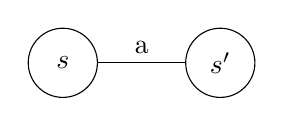
\begin{tikzpicture}[align=center,node distance=2cm]
    \node[state] (q1) {$s$};
    \node[state, right of=q1] (q2) {$s'$};
    \draw (q1) edge[above] node{a} (q2);
    \end{tikzpicture}
\par
} 

Oppure lo posso rappresentare elencando le diverse relazioni di transizioni. La relazione di transizione può essere estesa a una sequenza di azioni .
$$
s \stackrel{a}\to s' \; \text{ estesa a } \; s \stackrel{w}\to s' \; \text{ con } w \in Act^*
\iff 
$$
\begin{align*}
    \begin{cases} 
        \text{se } w=\epsilon & \text{allora }  s=s' \\
        \text{se } w=a \cdot x  \text{ con } a \in Act, x \in Act^*  & \text{allora } \text{ se } s \to^a s'' \to^x s'
    \end{cases}
\end{align*}

In generale diciamo che abbiamo $s \to s' $ sse $\exists a \in Act : s \stackrel{a} \to s'$, e quindi in qualche modo questa relazione $\quad \to \quad$, non etichettata, è uguale a $\displaystyle \bigcup\limits_{a\in Act}\stackrel{a}{\rightarrow}$. \\
Possiamo fare lo stesso per $s \to^* s'$ sse $\exists w \in Act^* : s \stackrel{w} \to s'$, e quindi posso avere 
$\quad \to^* \quad$, non etichettata, uguale a $\displaystyle \bigcup\limits_{w\in Act^*}\stackrel{w}{\rightarrow}$.\\

La relazione $\rightarrow^*$ è la chiusura riflessiva e transitiva della relazione $\rightarrow$ (tale relazione non è simmetrica), avendo sempre $s\rightarrow^*s'$ ed essendo garantita la transitività.\\

\subsubsection{Piccolo ripasso}
Data una relazione binaria $R$ su $X$. $R \subseteq X \times X$ \begin{itemize}
    \item $R$ è \textbf{riflessiva} $\iff \forall x \in X \quad (x,x) \in R$ ovvero $xRx$ 
    \item $R$ è \textbf{simmetrica} $\iff$ se $(x,y) \in R$ allora $(y,x) \in R \quad \forall x,y \in X$ 
    \item $R$ è \textbf{transitiva} $\iff$ se $(x,y) \in R \land (y,z) \in R$ allora $(x,z) \in R$ 
\end{itemize}
Se $R$ è simmetrica, riflessiva e transitiva, allora è una relazione di equivalenza.
Una \textbf{classe di equivalenze} data un elemento $x \in X$ è l’insieme di tutti gli elementi di $X$ in relazione con esso: $[x] = \{y \in X \; | \; (x,y) \in R\}$. \\
L’insieme $X$ è ripartibile in classi di equivalenza in quanto costituiscono insiemi disgiunti. Infatti, due classi di equivalenza sono o esattamente uguali o la loro intersezione è nulla. L’unione di tutte le classi di equivalenza di $X$ è pertanto uguale a $X$. 

Siano $R, R', R''$ relazioni binarie su $X$, ovvero $R, R', R'' \subseteq X \times X$. $R'$ è la *chiusura riflessiva/simmetrica/transitiva* di $R$ sse: 
\begin{enumerate}
    \item $R \subseteq R'$
    \item $R'$ è riflessiva/simmetrica/transitiva
    \item $R'$ è la più piccola relazione che soddisfa i punti 1 e 2. Dire che è la più piccola relazione corrisponde a dire che $\forall R''$ se $R \subset R'' \land R''$ è riflessiva/simmetrica/transitiva, allora deve succedere che $R' \subseteq R''$
\end{enumerate}

\subsection{CCS}
Per definire il \textbf{Calculus of Communicating Systems (\textit{CCS})} puro (astraendo l'aspetto delle strutture dati etc$\ldots$) dobbiamo definire che abbiamo: 
\begin{itemize}
    \item $K$, ovvero un insieme di nomi di processi, che possono anche essere simboli di un alfabeto
    \item $A$, ovvero un insieme di nomi di azioni, che possono essere azioni di sincronizzazione con l’ambiente o tra componenti o azioni interne di sincronizzazione avvenuta tra due componenti.
    \item $\overline{A}$, ovvero l'insieme di nomi delle \textit{coazioni} contenute in $A$, $\forall\, a\in A \quad \exists \quad \overline{a}\in \overline{A}$, quindi:$\overline{A}=\{\overline{A}|\,a\in A\}$ ovviamente si ha che:$\overline{\overline{a}}=a$
    \item $Act=A\cup \overline{A}\cup \{\tau\}$ dove $\tau\not\in A$ corrisponde all'azione di sincronizzazione tra $a$ e $\overline{a}$. Le due azioni $A$ e $\overline{A}$ sono \textit{azioni osservabili} e lo possiamo indicare con: $\mathcal{L}=A\cup \overline{A}$, mentre $\tau$ non è osservabile.\\ Ricordando che osservare un'azione significa poter interagire con essa.
\end{itemize}
Le azioni osservabili si devono sincronizzare con altre componenti, mentre le azioni non osservabili sono il risultato di una sincronizzazione.
\subsubsection{Processi CSS}
Sono delle espressioni scritte in linguaggio CCS, e un sistema CSS è dato da un insieme di processi $p \in K$, questi processi saranno definiti dalla formula $p = \textnormal{espressione CSS}$ e avrò solo una equazione $\forall \ p \in K$. \\

Dato un sistema CCS con $Act = A \cup \overline{A} \cup \{\tau\}$ e un insieme di processi CCS, gli si va ad assegnare un LTS, che avrà ($S=\text{processi CCS}, Act, T, p_0$), tramite delle regole di inferenza, in cui si ha una premessa (o più), delle condizioni, delle conseguenze (o conclusioni). Dare un significato tramite LTS, regole di inferenza e sintassi è detto
\textbf{semantica operazionale strutturale}.

Un processo CCS può essere:
\begin{itemize}
    \item \textbf{Nil} (0): corrisponde al sistema di transizioni con un unico stato etichettato “nil” senza nessuna transizione.
    \item \textbf{Operazione di prefisso}: $\alpha \cdot p$, dove $\alpha \in Act$ e $p \in \text{Processi CCS}$. La regola di inferenza associata è: \\ $\frac{}{\alpha \cdot p  \stackrel{\alpha}\to p}$
    \item \textbf{Operazione di somma} $p_1 + p_2$, dove $p_1, p_2 \in \text{Processi CSS}$.   Regola di inferenza: $p_1 \stackrel{\alpha}\to p'_1$. Il $+$ corrisponde alla scelta, quindi possiamo definire il comportamento con le regole di inferenza, con $\alpha$ e $\beta \ \in \ Act$ e $p_1 \ p_2 \in Proc_{CSS}$(processi CSS):
    \begin{itemize}
        \item Se sappiamo che $p_1$  può eseguire $\alpha$ e poi comportarsi come $p_1'$, allora $p_1 + p_2$ può eseguire $alpha$. $\frac{p_1 \stackrel{\alpha}\to p_1'}{p_1 + p_2 \stackrel{\alpha}\to p_1'}$
        \item Possiammo inoltre eseguire $\beta$, e seguendo lo stesso ragionamento per $p_1$, ottenendo
         $\frac{p_2 \stackrel{\beta}\to p_2'}{p_1 + p_2 \stackrel{\beta}\to p_2'}$
    \end{itemize}
    \item \textbf{Somma di processi}, posso avere quindi multiple somme, nella forma $\displaystyle \sum_{i\in I}p_i$ con $P_i \in Poc_{CSS}$, in questo caso la regola di inferenza associata è: $\frac{p_j\stackrel{\alpha}{\to}p_j'}{\displaystyle \sum_{i\in I}p_i\stackrel{\alpha}{\to}p_j0},\,j\in I$. \\
    Si possono presentare diversi casi: 
    \begin{itemize}
        \item se $I= \varnothing$ avrò che $\displaystyle \sum_{i\in I}p_i=Nil$
    \end{itemize}
    \item \textbf{Composizione parallela} se $p_1$ e $p_2$ sono due processi gli posso mettere in composizione parallela. Quindi $p_1$, $p_2 \ \in Prco_{CSS}$. Anche qui abbiamo le regole di inferenza
    \begin{itemize}
        \item Se $p_1$ può eseguire $\alpha$ e poi comportarsi come $p_1'$, allora se io ho $p_1 | p_2$, il processo può eseguire $\alpha$ e poi comportarsi come $p_1 | p_2$. Ovvero sarà: $\frac{p_1 \stackrel{\alpha}\to p_1'}{p_1|p_2 \stackrel{\alpha}\to p_1'|p_2}$
        \item Possiamo avere la cosa simmetrica nel caso di $p_2$, risulta che: $\frac{p_2 \stackrel{\alpha}\to p_2'}{p_1|p_2 \stackrel{\alpha}\to p_1|p_2'}$, usiamo in questo caso sempre $\alpha$, ma essa potrebbe essere diversa nella due regole (come valore/concetto).
        \item Può succedere anche che $p_1$ possa eseguire una certa azione $a$, e che $p_2$ sia pronto ad eseguire la sua coazione $\overline{a}$. Questo significa che sono entrambi pronti ad eseguire e possono tutti e due sincronizzarsi.
        $\frac{p_1 \stackrel{a}\to p_1' \land p_2 \stackrel{a}\to p_2'}{p_1|p_2 \stackrel \tau\ \to p_1'|p_2'}$, usiamo $\tau$ nella conseguenza perché vuol dire che i due processi si sincronizzano e $a$ si sincronizza con $\overline{a}$.
    \end{itemize}
    \item \textbf{Operazione di restrizione}, Supponiamo che $L$ sia un sottoinsieme dell'azione $A$, e che $P$ appartenga ai processi $P \in Proc_{CSS}$. Abbiamo quindi $P_{\setminus L}$, significa che  il processo $P$ non può interagire con il suo ambiente con azioni in $L \cup \overline{L}$ , ma le azioni in $L \cup \overline{L}$ sono locali a $P$.
    $\frac{p\stackrel{\alpha}{\to}p'}{p_{\setminus L} \stackrel{\alpha}{\to}p'_{\setminus L}} \quad \alpha,\overline{\alpha}\not\in L,\quad \textnormal{abbiamo che }L\subseteq A$
    
    \item \textbf{Rietichettatura}, $p_{[f]}$, operazione che serve per cambiare il nome ad alcune azioni per poter riutilizzare una specifica di un processo, magari all’interno di un altro sistema dove sono stati usati nomi diversi. Ho quindi una funzione $f$ tale che: $f:Act \to Act$. Ci sono alcune regole che devo garantire:
    \begin{itemize}
        \item $f(\tau) = \tau$
        \item $f(\overline{a}) = \overline{f(a)}$
    \end{itemize}
    Ho quindi $p_{[f]}$ tale che:  $\frac{p \stackrel  {\alpha} \to p'}{p_{[f]} \stackrel{f(\alpha)} \longrightarrow p_{[f]}' }$. Può presentarsi la situazione dove dato un nome di processo $k$, se $k = p$, allora $\frac{p \stackrel  {\alpha} \to p'}{k \stackrel  {\alpha} \to p'} \, \ k = p$. \\
    Quindi dato un CCS posso associare un LTS per quanto riguarda la semantica.
\end{itemize}
\section{Lezione 30 ottobre}
Dato un CCS abbiamo visto che è possibile associarli un LTS per quanto riguarda la semantica.\\ Si ha una \textbf{precedenza degli operatori}, da quello con meno precedenza a quello con più precedenza: \begin{enumerate} 
    \item restrizione, $\setminus_L$
    \item rietichettatura, $[f]$
    \item prefisso, $\alpha \cdot p$
    \item composizione parallela, $|$
    \item somma, $+$
\end{enumerate}
Vediamo più nel dettaglio la \textbf{composizione parallela}. Nel caso dovessimo avere la situazione $a \cdot NIL | \overline{a} \cdot NIL$, che si traduce nel LTS:

\begin{center}
    \begin{tikzpicture}[shorten >=1pt,node distance=4cm,on grid,auto]
      \node[state] (q_0) {\footnotesize{$a\cdot Nil\,\,|\,\,\overline{a}\cdot
          Nil$}}; 
      \node[state] (q_1) [below right=of q_0] {\footnotesize{$a\cdot
          Nil\,\,|\,\,Nil$}};  
      \node[state] (q_3) [below left=of q_0]
      {\footnotesize{$Nil\,\,\,\,|\,\,\overline{a}\cdot Nil$}}; 
      \node[state] (q_2) [below right =of q_3] {\footnotesize{$Nil|Nil$}};
      \path[->]
      (q_0) edge  node {$\overline{\alpha}$} (q_1)
      (q_1) edge  node {$\alpha$} (q_2)
      (q_3) edge  node [below left]{$\overline{\alpha}$} (q_2)
      (q_0) edge  node [above left]{$\alpha$} (q_3)
      (q_0) edge  node [above left] {$\tau$} (q_2);
    \end{tikzpicture}
  \end{center}
Dall'esempio sopra noto che posso quindi eseguire le due operazioni o in una sequenza o nell'altra.\\ 
Ho quindi una \textbf{simulazione sequenziale non deterministica} del comportamento del sistema dato dalla composizione parallela.\\
Con quanto visto in questo esempio è possibile perché nell'ipotesi di Milner si ha
che $a$ e $\overline{a}$ sono \textbf{operazioni atomiche}.

Si hanno anche modelli di CCS modellati con:  reti di Petri e strutture ad eventi. Sono due modelli in cui si considera la semantica basata sulla \textbf{true concurrency}, a \textit{ordini parziali}, ovvero non si impongono sequenze quindi due processi o si sincronizzano o vengono eseguiti in maniera indipendente/concorrente con l'ambiente.

\subsection{Esempio dell'altra volta}
Costruisco il sistema di transizioni della specifica: $S=\overline{lez}\cdot S$ 

\begin{center} 
    \begin{tikzpicture}[shorten >=1pt,node distance=2cm,on grid,auto] 
        \node[state] (q_0) {$S$}; 
        \path[->] (q_0) edge [loop right]  node {$\overline{lez}$} (q_0); 
        \end{tikzpicture} 
\end{center} avendo: 
$\displaystyle Uni=(M|LP)_{\backslash\{ coin, caffe\}}$ ,seguendo nei vari step le regole di inferenza legate alla sincronizzazione: \\

$\displaystyle (coin\cdot \overline{caffe}\cdot M \ | \ \overline{lez}\cdot\overline{coin}\cdot caffe\cdot LP)_{\backslash\{ coin, caffe\}}$, eseguendo il passo $\overline{lez}$, mi ritrovo nella fase : \\

$\displaystyle (coin\cdot \overline{caffe}\cdot M \ | \ \overline{coin}\cdot caffe\cdot LP)_{\backslash\{ coin, caffe\}}$, e visto che $coin$ e $\overline{coin}$ non può essere eseguito con l'ambiente, i due processi si sincronizzano sul $coin$ con una $\tau$: \\

$\displaystyle (\overline{caffe}\cdot M \ | \ \cdot caffe\cdot LP)_{\backslash\{ coin, caffe\}}$, a questo punto dobbiamo sincronizzarci con $caffe$, anche in questo caso con una $\tau$: 
$\displaystyle ( M \ | \  LP)_{\backslash\{ coin, caffe\}}$ che mi riporta allo stato iniziale. Ricordiamo che le due $\tau$ sono diverse.

La domanda che possiamo porci è: Data una implementazione, che corrisponde agli step eseguiti, questa implementazione soddisfa la nostra specifica, $S$, oppure no?
Innanzitutto per poter dire che una certa implementazione soddisfa (indicata con $implementazione \models specifica$) una certa specifica o se due implementazioni diverse soddisfano la stessa specifica ci serve una \textbf{relazione di equivalenza} tra processi CCS, ovvero una $R$: $R\subseteq P_{CCS}\times P_{CCS}$ che sia riflessiva, simmetrica e transitiva.
Bisognerà inoltre astrarre: gli stati e considerare le azioni $Act$, dalle sincronizzazioni interne, ovvero dalle $\tau$ e  rispetto al non determinismo. Milner poi asserisce che $R$ deve essere inoltre una \textbf{congruenza} rispetto agli operatori del CCS.\\

\subsection{Relazione di equivalenza}
Una relazione di equivalenza $R$ è una \textbf{congruenza} sse:$\forall \,\,p,q\in Proc_{CCS} \land \forall c[\cdot] \mbox{ contesto CCS}$, se $p\ R \ q$, allora deve succedere che se io prendo il contesto con all'interno il processo $p$, $C[p]$, e al posto di $p$ sostituisco $q$ allora il contesto $C[q]$ deve essere in relazione con $C[p]$. ($C[q] \ R \ C[p])$.

Dati due processi $p_1$ e $p_2$ a cui assegniamo i due LTS $v_1$ e $v_2$. I due processi sono equivalenti se $v_1$ e $v_2$ sono isomorfi. Possiamo in realtà cercare qualcosa di meno forte rispetto all'isomorfismo ma che garantisca lo stesso risultato. Si va a vedere quindi se i due LTS \textbf{ammettono le stesse sequenze di operazioni}, prendendo l'\textbf{equivalenza forte} tra automi a stati finiti. Questa è detta \textbf{equivalenza rispetto alle tracce}. È comunque più forte di dire che hanno la stessa precondizione e postcondizione.\\ Bisognerà trattare il problema dal punto di vista della congruenza. 

\subsection{Equivalenza rispetto alle tracce}
Innanzitutto prendo un processo $P \in Proc_{CSS}$ e dico quali sono le tracce di P, $Tracce(P)$. Prendo un processo, prendo un transition system e prendo, non il linguaggio accettato, ma prendo tutte le sequenze di azioni che sono possibili da parte del processo $P$.\\ $Trace(P) = \{w \in \ Act^* \ t.c: \ \exists \ p' \in Proc_{CSS} \ p \stackrel{w} \to p' \}$\\

Preso $P_1\in Proc_{CCS}$ ho che è equivalente rispetto alle tracce a $P_2$, scritto: $P_1 \ \stackrel{T}{\sim} \  P_2$ sse: \\ $Tracce(P_1) = Tracce (P_2)$. Quindi le sequenze di azioni possibili da $P_1$ possono essere fatte anche da $P_2$

\subsubsection{Esempio macchinetta del caffè} 
Prendiamo $(LP|M_i)_{\backslash\{coin, caff\textnormal{è}\}}$ suppongo di avere due macchinette $M$ che erogano sia caffè che $tea$, per il primo basta una moneta e per il secondo due. \\
 
$M_1 = \overline{coin} \cdot (caff\textnormal{\textit{è}} \cdot M_1 + \overline{coin} \cdot tea \cdot M_1)$ \\
$M_2 = \overline{coin} \cdot caff\textnormal{\textit{è}} \cdot M_2 + \overline{coin} \cdot \overline{coin} \cdot tea \cdot M_2$ \\
Le tracce di $M_1$ sono o non sono le stesse di $M_2\stackrel{?}{=} M_1 \ \stackrel{T}{\sim} \ M_2$
Partiamo a considerare prima $M_1$
 \begin{center}
    \begin{tikzpicture}[shorten >=1pt,node distance=5cm,on grid,auto]
      \node[state] (q_0) {$M_1$}; 
      \node[state] (q_1) [below=of q_0] {\footnotesize{$caffe\cdot M_1+\overline{coin}\cdot tea\cdot M_1$}};  
      \node[state] (q_2) [right=of q_1]
      {$tea\cdot M_1$}; 
      
      \path[->]
      (q_0) edge  node {$\overline{coin}$} (q_1)
      (q_1) edge  node [above]{$\overline{coin}$} (q_2)
      (q_2) edge  node [above right] {$tea$} (q_0)
      (q_1) edge [bend left= 25] node [above left] {$caffe$} (q_0);
    \end{tikzpicture}
  \end{center}
Consideriamo ora invece $M_2$
\begin{center}
    \begin{tikzpicture}[shorten >=1pt,node distance=4cm,on grid,auto]
     \node[state] (q_0) {$M_2$}; 
      \node[state] (q_1) [below right=of q_0] {$\overline{coin}\cdot tea\cdot M_2$};
      \node[state] (q_2) [below left=of q_0] {$caffe\cdot M_2$};
      \node[state] (q_3) [above right=of q_0] {$tea\cdot M_2$}; 
      
      \path[->]
      (q_0) edge  node {$\overline{coin}$} (q_2)
      (q_0) edge  node {$\overline{coin}$} (q_1)
      (q_1) edge [right] node {$\overline{coin}$} (q_3)
      (q_3) edge  node {$tea$} (q_0)
      (q_2) edge [bend left= 25] node [above left] {$caffe$} (q_0);
    \end{tikzpicture}
\end{center}

Si vede quindi che le tracce di $M_1$ sono le stesse di quelle di $M_2$. Vuol dire che $M_1 \ \stackrel{T}{\sim} \ M_2$. Se sostituisco le due macchine si nota che $M_2$ può andare in deadlock, avendo due processi che iniziano con $\overline{coin}$, infatti la macchina potrebbe aspettare una seconda moneta per prendere il $tea$, mentre magari volevo il $caff\textnormal{\textit{è}}$. Questo perché $M_2$ ha un comportamento non deterministico. \\

Lo studio delle tracce quindi non è più sufficiente nel caso di sistemi concorrenti. Si necessità quindi di una nozione più restrittiva.\\ Per ovviare al problema sopra descritto si ha la \textbf{bisimulazione}. 
$M_1$ e $M_2$ non sono equivalenti rispetto alla \textbf{bisimulazione} e quindi non posso sostituire l'una con l'altra: $M_1\stackrel{Bis}{\not\sim}M_2$
\section{Lezione del 2 novembre} 
Esercizio, creare la LTS di $x = ((a \cdot P_1' +  \overline{b}\cdot P_1'')|((a \cdot P_1' +  \overline{b}\cdot P_1''))_{\backslash\{a\}}$
\begin{center}
    \begin{tikzpicture}[shorten >=1pt,node distance=7cm,on grid,auto]
      \node[state] (q_0) {$((a \cdot P_1' +  \overline{b}\cdot P_1'')|((a \cdot P_1' +  \overline{b}\cdot P_1''))_{\backslash\{a\}}$}; 
      \node[state] (q_1) [below=of q_0] {{$(P_1'')|((a \cdot P_1' +  \overline{b}\cdot P_1''))_{\backslash\{a\}}$}}; 
      \node[state] (q_2) [below left =of q_0] {$(P_1' | P_2')_{\backslash\{a\}}$};  
      \node[state] (q_3) [right = of q_0] {$( (a \cdot P_1' +  \overline{b}\cdot P_1'') | P_2')_{\backslash\{a\}}$};  
      \node[state] (q_4) [below right = of q_0] {$(P_1'' | P_2'')_{\backslash\{a\}}$};
      \path[->] 
      (q_0) edge  node {$\overline{b}$} (q_1)
      (q_0) edge  node {$\tau$} (q_2)
      (q_0) edge  node {$b$} (q_3)
      (q_0) edge  node {$\tau \textnormal{di b}$} (q_4)
      (q_1) edge  node {$b$} (q_4)
      (q_3) edge  node {$\overline{b}$} (q_4);
    \end{tikzpicture}
\end{center}

Altri esempi: 
$P_1=a\cdot b\cdot Nil+a\cdot c\cdot Nil$ e $P_2=a\cdot(b\cdot Nil+c\cdot Nil)$.
Per il caso $P_1$
\begin{center}
    \begin{tikzpicture}[shorten >=1pt,node distance=2.5cm,on grid,auto]
        \node[state] (q_0) {$P_1$}; 
        \node[state] (q_1) [below right=of q_0] {$c\cdot Nil$};  
        \node[state] (q_3) [below left=of q_0]
        {$b\cdot Nil$}; 
        \node[state] (q_2) [below right =of q_3] {$Nil$};
        \path[->]
        (q_0) edge  node {$a$} (q_1)
        (q_1) edge  node {$c$} (q_2)
        (q_3) edge  node [below left]{$b$} (q_2)
        (q_0) edge  node [above left]{$a$} (q_3);
    \end{tikzpicture}
\end{center}
Avendo come trace $Trace(P_1) = \{\epsilon,a ,ab, ac\}$ \\
Per il caso $P_2$
\begin{center}
    \begin{tikzpicture}[shorten >=1pt,node distance=2.4cm,on grid,auto]
        \node[state] (q_0) {$P_2$}; 
        \node[state] (q_1) [below=of q_0] {$b\cdot Nil+c\cdot Nil$};  
        \node[state] (q_2) [below=of q_1] {$Nil$}; 
        \path[->]
        (q_0) edge  node {$a$} (q_1)
        (q_1) edge [bend right = 25] node[below left] {$b$} (q_2)
        (q_1) edge [bend left = 25] node {$c$} (q_2);
    \end{tikzpicture}
\end{center}
E notiamo che le tracce di $P_2$ siano le stesse, quindi $P_1 \stackrel{T}{\sim} P_2$. \\
Ma se ad esempio prendo:
  $Q_1=(P_1|\overline{a}\cdot \overline{c}\cdot Nil )_{\backslash\{a,b,c\}}$
  $Q_2=(P_2|\overline{a}\cdot \overline{c}\cdot Nil )_{\backslash\{a,b,c\}}$
  Ho:
\begin{center}
    \begin{tikzpicture}[shorten >=1pt,node distance=4cm,on grid,auto] 
        \node[state] (q_0) {$Q_1$};  
        \node[state] (q_1) [below right=of q_0] {$(b\cdot Nil+\overline{c} \cdot Nil)_{\backslash\{a,b,c\}}$};
        \node[state] (q_3) [below left=of q_0] {$(c\cdot Nil+\overline{c} \cdot Nil)_{\backslash\{a,b,c\}}$}; 
        \node[state] (q_2) [below =of q_3] {$Nil|Nil$};
        \node[state] (q_4) [below =of q_1] {$deadlock$};
        \path[->]
        (q_0) edge  node {$\tau$} (q_1)
        (q_0) edge  node [above left] {$\tau$} (q_3)
        (q_3) edge  node {$\tau$} (q_2)
        (q_1) edge  node {$\tau$} (q_4);
    \end{tikzpicture}
\end{center}
\begin{center}
    \begin{tikzpicture}[shorten >=1pt,node distance=4cm,on grid,auto]
        \node[state] (q_0) {$Q_2$}; 
        \node[state] (q_1) [below=of q_0] {$(b\cdot Nil+c\cdot Nil|c\cdot Nil
        )_{\backslash\{a,b,c\}}$}; 
        
        \node[state] (q_2) [below=of q_1] {$Nil|Nil$}; 
        \path[->]
        (q_0) edge  node {$\tau$} (q_1)
        (q_1) edge  node {$\tau$} (q_2);
    \end{tikzpicture}
\end{center}
Quindi il primo va in deadlock e il secondo no, quindi vedremo non sono
equivalenti per la bisimulazione.
  
%%questo esempino non lo metto, non serve secondo me, era >> quello prima

\subsection{Bisimulazione}
Data una relazione binaria $R\subseteq Proc_{CCS}\times Proc_{CCS}$, questa è una relazione di bisimulazione (forte) sse: $\forall \ p,q\in Proc_{CCS} \ t.c: \ p \ R \ q \mbox{ vale quanto segue }$: 
\begin{itemize} 
    \item $\forall \alpha\in Act=A\cup \overline{A} \cup \{\tau\}$ se ho $p\stackrel{\alpha}{\rightarrow}p'$ allora deve esistere un $ q'\in  Proc_{CCS} \mbox{ t.c }q\stackrel{\alpha}{\rightarrow}q'\mbox{ e si ha }p'\ R\ q'$ 
    \item  $\forall \alpha\in Act=A\cup \overline{A}\cup \{\tau\}$ se ho $q\stackrel{\alpha}{\rightarrow}q'$ allora deve esistere un $ p' \in  Proc_{CCS}\mbox{ t.c }p\stackrel{\alpha}{\rightarrow}p'\mbox{ e si ha }p'\ R\ q'$ 
\end{itemize} 
Due processi $p$ e $q$ sono fortemente bisimili: $p\stackrel{Bis}{\sim} q$ sse $\exists \ R\subseteq Proc_{CCS}\times Proc_{CCS}$, relazione di bisimulazione forte tale che $p \ R\ q$.\\ 

Possiamo dire che in generale : $\stackrel{Bis}{\sim}=\cup\{R\subseteq Proc_{CCS}\times Proc_{CCS} | \ R \mbox{ è una relazione di bisimulazione forte}\}$

\subsubsection{Teorema bisimulazione forte}
Se prendo $\stackrel{Bis}{\sim}\subseteq Proc_{CCS}\times Proc_{CCS}$ si dimostra che questa è una relazione riflessiva, simmetrica e transitiva. Quindi è una relazione di equivalenza.\\ 

Posso scrivere quindi che: 
$p\stackrel{Bis}{\sim} q 
    \begin{cases}
         \iff \forall\alpha\in Act \\
         \land \textnormal{devono valere entrambe}\begin{cases}
             \textnormal{se } p\stackrel{\alpha}{\rightarrow}p' \mbox{ allora } \exists q':
             q\stackrel{\alpha}{\rightarrow}q'\land p'\stackrel{Bis}{\sim}q' \\
             \textnormal{se } q\stackrel{\alpha}{\rightarrow}q' \mbox{ allora } \exists p': p\stackrel{\alpha}{\rightarrow}p'\land p'\stackrel{Bis}{\sim}q'
         \end{cases}
    \end{cases}
$

Se due processi sono fortemente bisimili allora sono sicuramente equivalenti rispetto alle tracce. Il viceversa non vale, esistono infatti processi equivalenti rispetto alle tracce che non sono bisimili.  Per vedere che due processi sono bisimili devo quindi, per ogni esecuzione, ottenere due processi ancora bisimili.

%%%% fa esempi, se vuoi posso fare le immagini che mi viene facile poi fare il pdf, però non mi sembravano molto necessari questi

Ricavando le tracce di due processi possiamo in alcuni casi osservare una traccia $\tau$, quello che devo fare è poter quindi di astrarre dalle interazioni interne ($\tau$), introducendo l'\textbf{equivalenza debole}, volendo astrarre rispetto alle azioni $\tau$, introducendo la \textbf{bisimulazione debole}.
\section{Lezione del 4 novembre}
\subsection{Esempio utilizzando Buffer}
Cerco quindi di astrarre dalle interazioni interne ($\tau$), introducendo l'\textbf{equivalenza debole}, volendo astrarre rispetto alle azioni $\tau$, introducendo la \textbf{bisimulazione debole} (e nell'esempio precedente i due processi sono debolmente equivalenti sia per le tracce che per la bisimulazione).
Vediamo l'esempio dei buffer, dato un buffer di capacità $r$ che contiene $i$ elementi ho $B_i^R$.\\ Sia quindi, su $A=\{in,out\},\quad \overline{A}=\{\overline{in},\overline{out}\}$, con $A$ per azioni di ricezione e $\overline{A}$ per azioni di invio, il buffer a capacità 1: $B_0^1=in\cdot B_1^1$, $B_1^1=\overline{out}\cdot  B_0^1$. Avendo il corrispondente LTS nella figura [\ref{figura_lts_buffer1}] \\
Passo poi successivamente al buffer a capacità 2, e abbiamo $B_0^2=in \cdot B_1^2$, $B_1^2=\overline{out} \cdot B_0^2+in \cdot B_2^2$, $B_2^2=\overline{out}\cdot B_1^2$: questo corrisponde ad avere un LTS che si presenta come in figura [\ref{figura_lts_buffer2}]\\
\begin{figure}[ht]
\centering
    \begin{minipage}[b]{0.3\textwidth}
    \centering
    \begin{tikzpicture}[shorten >=1pt,node distance=2cm,on grid,auto] 
        \node[state] (q_0) {$B_0^1$};  
        \node[state] (q_1) [below =of q_0] {$B_1^1$};
        
        \path[->]
        (q_0) edge [bend right = 25]node[left] {$in$} (q_1)
        (q_1) edge [bend right = 25] node [right]{$\overline{out}$} (q_0)
        ;
    \end{tikzpicture}
    \caption{LTS rappresentante Buffer 1}
    \label{figura_lts_buffer1}
    \end{minipage}
    \hspace{3cm}% NO SPACE!
    \begin{minipage}[b]{0.3\textwidth}
    \centering
       \begin{tikzpicture}[shorten >=1pt,node distance=2cm,on grid,auto] 
          \node[state] (q_0) {$B_0^2$};  
          \node[state] (q_1) [below =of q_0] {$B_1^2$};
          \node[state] (q_2) [below =of q_1] {$B_2^2$};
          \path[->]
          (q_0) edge [bend right = 25]node[left] {$in$} (q_1)
          (q_1) edge [bend right = 25] node [right]{$\overline{out}$} (q_0)
          (q_1) edge [bend right = 25]node[left] {$in$} (q_2)
          (q_2) edge [bend right = 25] node [right]{$\overline{out}$} (q_1)
          ;
        \end{tikzpicture}
    \caption{LTS rappresentante Buffer 2}
    \label{figura_lts_buffer2}
    \end{minipage}
\end{figure}

Provo ora a sincronizzare due buffer a capacità 1: $B_0^1|B_0^1$. Avendo il corrispondente LTS, non avendo la sincronizzazione:
\begin{center}
    \begin{tikzpicture}[shorten >=1pt,node distance=3.5cm,on grid,auto] 
        \node[state] (q_0) {$B_0^1|B_0^1$};  
        \node[state] (q_1) [below left =of q_0] {$B_1^1|B_0^1$};
        \node[state] (q_2) [below right =of q_0] {$B_0^1|B_1^1$};
        \node[state] (q_3) [below right =of q_1] {$B_1^1|B_1^1$};
        \path[->]
        (q_0) edge [bend right = 25] node [above left]{$in$} (q_1)
        (q_0) edge [bend left = 25] node[above right]{$in$} (q_2)
        (q_1) edge [bend right = 25] node [above left]{$\overline{out}$} (q_0)
        (q_2) edge [bend left = 25] node [above right]{$\overline{out}$} (q_0)
        (q_1) edge [bend right = 25] node [below left]{$in$} (q_3)
        (q_2) edge [bend left = 25] node [below right]{$in$} (q_3)
        (q_3) edge [bend right = 25] node [below left]{$\overline{out}$} (q_1)
        (q_3) edge [bend left = 25] node [below right]{$\overline{out}$} (q_2)
        ;
    \end{tikzpicture}
\end{center}
Si ha quindi, in quest'ultimo modello, una \textbf{simulazione sequenziale non deterministica della concorrenza}.\\ Vediamo se si ha che: $(B_0^1|B_0^1)\stackrel{Bis}{\sim}B_0^2$, notiamo che $B_0^2$ può essere messo in relazione con $B_0^1|B_0^1$ in quanto se vado in uno tra $B_1^1|B_0^1$ e $B_0^1|B_1^1$ posso sempre fare $in $ e $\overline{out}$. Inoltre Posso fare un discorso analogo per $B_2^2$ e $B_1^1|B_1^1$. Essendo questi ultimi quindi bisimili lo sono anche il nodo centrale coi due possibili nodi nel caso della composizione e di conseguenza lo sono anche $B_0^2$ e $B_0^1|B_0^1$. Diciamo in questo modo che sono bisimili il LTS del buffer a due posizioni [\ref{figura_lts_buffer2}] sequenziale e quello a due contenitori diversi a una postazione.(sopra)
Proprietà della bisimulazione forte:
\begin{itemize}
    \item La bisimulazione forte è una congruenza rispetto agli operatori del CCS.
        Se $p \stackrel{Bis}{\sim} q$ con $p,q \in Proc_{CCS}$, allora: 
        \begin{itemize}
            \item $\forall \alpha \in Act$, $\; \alpha \cdot p \stackrel{Bis}{\sim} \alpha \cdot q$, dove $\alpha$ è un contesto
            \item $\forall r \in Proc_{CCS}$, $\; p + r \stackrel{Bis}{\sim} q +r \; \land \; r + p \stackrel{Bis}{\sim} r + q$, ricordiamo che in questo caso abbiamo che $+$ è il contesto preso in considerazione
            \item $\forall \alpha \in Act$, $\; p | r \stackrel{Bis}{\sim} q|r \; \land \; r | p \stackrel{Bis}{\sim} r | q$, il contesto è la composizione parallela $|$
            \item $\forall f : Act \to Act$ funzione di rietichettatura, $\; p_{[f]} \stackrel{Bis}{\sim} q_{[f]}$, si ricorda che deve valere che la funzione $f$ è tale che $f(\tau) = \tau$ e $f(\overline a) = \overline{f(a)}$
            \item $\forall L \in A$, $\; p_{\setminus L} \stackrel{Bis}{\sim} q_{\setminus L}$
        \end{itemize}
\end{itemize}
Per gli operatori che abbiamo osservato prima, ci sono delle proprietà avendo sempre con $p,q,r \in Proc_{CCS}$:
\begin{itemize}
    \item Proprietà commutativa: 
        \begin{itemize}
            \item $p + q \stackrel{Bis}{\sim} q + p$
            \item $p | q \stackrel{Bis}{\sim} q | p$
        \end{itemize}
    \item Proprietà distributiva:
        \begin{itemize}
          \item $(p + q) + r \stackrel{Bis}{\sim} p + (q + r)$
          \item $(p | q) | r \stackrel{Bis}{\sim} p | (q | r)$
        \end{itemize}
    \item Leggi di assorbimento:
        \begin{itemize}
          \item $p + Nil \stackrel{Bis}{\sim} p$
          \item $p | Nil \stackrel{Bis}{\sim} p$
        \end{itemize}
\end{itemize}
\subsection{Equivalenza debole rispetto alle tracce}
Si vuole poter astrarre rispetto alle sincronizzazioni interne ($\tau$). Questo perché la bisimulazione forte rischia di essere troppo restrittiva. Motivazione per quale si passa quindi all’equivalenza debole rispetto alle tracce, $\stackrel{T}{\approx}$, e alla bisimulazione debole, $\stackrel{Bis}{\approx}$.\\
Per poterlo fare bisogna cambiare la regola di transizione, passando da $p\stackrel{a}{\rightarrow}p'$ a $p\stackrel{a}{\Rightarrow}p'$. \\
Dove $p\stackrel{a}{\Rightarrow}p'$ sta a indicare che $p$ interagisce sicuramente con l’ambiente attraverso $a$, ma prima o dopo potrebbe fare un numero qualsiasi di sincronizzazioni interne $\tau$; dopodiché si comporta come $p'$.
\subsubsection{Relazione/regola di transizione debole}
Definiamo la nostra relazione/regole di transizione debole nel modo: $\Rightarrow\subseteq Proc_{CCS}\times Act\times Proc_{CCS}$. \\ Quindi $p\stackrel{a}{\Rightarrow}p'$, con $a\in A\cup \overline{A}\cup \tau \iff$
\begin{enumerate}
    \item se $a=\tau$, allora $p\stackrel{\tau}{{\to}{^*}}p'$, ovvero è possibile eseguire una sequenza qualsiasi anche nulla di $\tau$, arrivando a $p'$, questo lo possiamo classificare dicendo 
    $\begin{cases}
        \textnormal{Se } a = 0 & \textnormal{ allora } $p=p'$. \\
        \textnormal{oppure } & p\stackrel{\tau}{\rightarrow} \; \dots \; \stackrel{\tau}{\rightarrow}p'.
    \end{cases} 
    $
    \item  se $\alpha\in A\cup\overline{A}$, allora $p\stackrel{\tau}{\rightarrow^*} \; \stackrel{\alpha}{\rightarrow}\; \stackrel{\tau}{\rightarrow^*}p'$.

\end{enumerate}
Estendiamo ora la relazione a sequenze di azioni $\forall w \in Act^*$: 
$p\stackrel{w}{\Rightarrow}p' \iff$ vale una delle due casistiche:
\begin{enumerate}
    \item se $w=\varepsilon$ (sequenza vuota) $\; \lor \; w=\tau^*$ (sequenza di $\tau$), allora in questo caso posso dire che $p\stackrel{\tau}{\Rightarrow^*}p'$.
    \item se $w=a_1\ldots a_n$, con $a_i\in A\cup \overline{A}$, allora $p\stackrel{a_1}{\Rightarrow}\cdots \stackrel{a_n}{\Rightarrow}p'$, dove ogni $a_i$ può essere preceduto/seguito da una qualsiasi sequenza di $\tau$.
\end{enumerate}
A questo punto possiamo avere come notazione, siano gli esempi:
\begin{itemize}
    \item $p\stackrel{ab}{\Rightarrow}p'$ potrebbe corrispondere a: $p\stackrel{\tau}{\rightarrow^*}p_2\stackrel{a}{\rightarrow}p_3\stackrel{\tau}{\rightarrow^*}p_4\stackrel{b}{\rightarrow}p_5\stackrel{\tau}{\rightarrow^*}p'$, dove $p_1$ e $p_2$ possono essere lo stesso. 
    \item $p_1\stackrel{\varepsilon}{\Rightarrow}p_1'$, in questo caso significa che: 
    $p_1 = p_1' \lor p\stackrel{\tau}{\rightarrow^*}p_1'$ questa è equivalente al fatto di scrivere 
    $p_1\stackrel{\tau}{\Rightarrow}{p_1}'$
\end{itemize}
\textbf{Equivalenza debole rispetto alle tracce con regola debole} \\
$p\stackrel{T}{\approx} q \iff Tracce_{\Rightarrow}(p)=Tracce_{\Rightarrow}(q)$ ovvero $\forall w\in(A\cup \bar{A})^*$, se ho che posso eseguire $p\stackrel{w}{\Rightarrow} \ \iff \ q\stackrel{w}{\Rightarrow}$ (i due processi possono fare la stessa sequenza). Possiamo quindi a dire: $p\stackrel{w}{\Rightarrow} \equiv \exists p' : \ p\stackrel{w}{\Rightarrow} p'$. \\
Dove $Tracce_{\Rightarrow}(p)=\{w\in(a\cup \overline{A})^*| p\stackrel{w}{\Rightarrow}\}$.
Quindi o si hanno le stesse tracce con la regola debole o ogni sequenza del primo processo deve trovarsi nel secondo processo. Banalmente si prendono le tracce forti e si cancella $\tau$.
\section{Lezione del 9 novembre}
\subsection{Bisimulazione debole}

Una relazione $R\subseteq Proc_{CCS}\times Proc_{CCS}$ è una bisimulazione debole $\iff \forall p,q \in Proc_{CCS} \; | \; pRq$, vale che $\forall a\in Act = A \cup \bar{A} \cup \{\tau\}$,
\begin{itemize}
    \item se $p\stackrel{a}{\rightarrow}p_1$, allora esiste $q\stackrel{a}{\Rightarrow}q_1$ tale che $p_1Rq_1$
    \item se $q\stackrel{a}{\rightarrow}q_1$, allora esiste $p\stackrel{a}{\Rightarrow}p_1$ tale che $p_1Rq_1$
\end{itemize}

Quindi due processi $p$ e $q$ sono in \textbf{bisimulazione debole} $(p\stackrel{bis}{\approx}q) \iff \exists$ una relazione di bisimulazione $R$ tale che $pRq$. E quindi la relazione di bisimulazione è corrispondente a:
$$\stackrel{Bis}{\approx} =\bigcup\{R \; | \; R\textnormal{ è di bisimulazione debole} \}$$

\subsection{Bisimulazione debole come gioco} 
Regole del gioco che spiegano come capire se due processi sono bisimili. Per confrontare due processi CCS, $p$ e $q$, è possibile usare un gioco $G(p,q)$ con due giocatori, quali:
\begin{enumerate}
    \item attaccante: cerca di dimostrare $p\stackrel{Bis}{\not\approx}q$
    \item difensore: cerca di dimostrare $p\stackrel{Bis}{\approx}q$
\end{enumerate}
Un gioco è costituito da più partite, ognuna delle quali consiste in una sequenza finita o infinita di configurazioni o \textit{mani} $(p_0,q_0), \dots, (p_i,q_i) \dots$.
In ogni mano si passa dalla configurazione corrente a quella successiva tramite diverse regole:
\begin{itemize}
    \item l’attaccante sceglie uno dei processi della configurazione corrente $(p_i,q_i)$ e fa una $\stackrel{a}{\rightarrow}$ mossa ($a \in Act)$ con la regola forte.
    \item il difensore deve rispondere con una \textit{mossa} $\stackrel{a}{\Rightarrow}$ con la regola debole, sull’altro processo.
\end{itemize}
La nuova coppia $(p_{i+1},q_{i+1})$ ottenuta in questo modo diventa la nuova configurazione corrente e la partita continua con l’altra mano. Se un giocatore non può più muovere l’altro vince; inoltre se la partita è infinita vince il difensore.
Diverse partire possono concludersi con vincitori diversi ma per ogni gioco un solo giocatore può vincere la partita. 

Una \textbf{strategia} per un giocatore è un insieme di regole che indicano di volta in volta che mossa fare e che dipendono solo dalla configurazione corrente.\\
Diciamo che un giocatore ha una \textbf{strategia vincete} se per $G(p,q)$, seguendo quella strategia, vince tutte le partite del gioco.
\begin{teorema}{Teorema}{}
    \par\centering
    Per ogni gioco $G(p,q)$ solo uno dei due giocatori ha una strategia vincente.
\end{teorema}
\begin{teorema}{Teorema}{}
    \par\centering
    L’attaccante ha una strategia vincente $\iff p \stackrel{Bis}{\not\approx}q$.\\
    Il difensore ha una strategia vincente $\iff p \stackrel{Bis}{\approx}q$.
\end{teorema}

A questo punto il gioco della bisimulazione può essere usato sia per dimostrare che due processi sono bisimili, sia per dimostrare che non lo sono:
\begin{itemize}
    \item per dimostrare che sono bisimili, bisogna mostrare che per ogni mossa dell’attaccante il difensore ha almeno una mossa che lo porterà a vincere.
    \item per vedere che non sono bisimili, bisogna dimostrare che in ogni configurazione l’attaccante è in grado di scegliere su quale processo operare e con quale azione, in modo tale che per ogni risposta del difensore l’attaccante avrà almeno una mossa che lo porterà a vincere.
\end{itemize}
\subsubsection{Esempio chiarificatore}
Vediamo l'esempio di un gioco con due processi che dimostreremo essere bisimili:\\
Siano:
\begin{itemize}
    \item $p_1=a\cdot(b\cdot Nil+\tau\cdot c\cdot Nil)$ (sinistra)
    \item $u_1=a\cdot(b\cdot Nil+\tau\cdot c\cdot Nil)+a\cdot c\cdot Nil$ (destra)
\end{itemize}
\begin{figure}[H]
    \centering
    \begin{minipage}[b]{.35\textwidth}
        \centering
        \begin{tikzpicture}[shorten >=1pt,node distance=2cm,on grid,auto] 
          \node[state] (q_0) {$q_1$};  
          \node[state] (q_1) [below left =of q_0] {$q_2$};
          \node[state] (q_2) [below right =of q_0] {$q_3$};
          \node[state] (q_3) [below right =of q_1] {$Nil$};
          \path[->]
          (q_0) edge [above left] node {$a$} (q_1)
          (q_0) edge  node {$a$} (q_2)
          (q_1) edge [below left] node {$b$} (q_3)
          (q_2) edge  node {$c$} (q_3)
          ;
        \end{tikzpicture}
        \caption{$p_1$}
        \label{fig:prob1_6_2}
    \end{minipage}%
    \begin{minipage}[b]{0.35\textwidth}
        \centering
        \begin{tikzpicture}[shorten >=1pt,node distance=2cm,on grid,auto] 
            \node[state] (q_0) {$u_1$};  
            \node[state] (q_1) [below= of q_0] {$u_2$};
            \node[state] (q_2) [left = of q_1] {$u_3$};
            \node[state] (q_3) [right  =of q_1] {$u_4$};
            \node[state] (q_4) [below =of q_1] {$Nil$};
            \path[->]
            (q_0) edge [above left] node {$a$} (q_1)
            (q_0) edge  node {$a$} (q_3)
            (q_1) edge  node {$b$} (q_4)
            (q_1) edge  node {$\tau$} (q_2)
            (q_2) edge [below left] node {$c$} (q_4)
            (q_3) edge [below right] node {$c$} (q_4)
            ;
        \end{tikzpicture}
        \caption{$u_1$}
        \label{fig:prob1_6_1}
    \end{minipage}
\end{figure}
Vediamo quindi come si svolgono tutte le partite per $G(p_1,u_1)$:
\begin{itemize}
    \item all'inizio l'attaccante può fare $p_1\stackrel{a}{\rightarrow}p_2$ e il difensore può fare $u_1\stackrel{a}{\Rightarrow}u_2$, ed è la scelta vincente, avendo che $p_2$ e $u_2$ sono isomorfi. Una scelta buona su tre possibilità
    \item all'inizio l'attaccate può fare $u_1\stackrel{a}{\rightarrow}u_2$ e il difensore può fare $p_1\stackrel{a}{\Rightarrow}p_2$, ed è la scelta vincente, avendo che $p_2$ e $u_2$ sono isomorfi. Una scelta buona su due possibilità
    \item all'inizio l'attaccate può fare $u_1\stackrel{a}{\rightarrow}u_4$ e il difensore può fare $p_1\stackrel{a}{\Rightarrow}p_3$, ed è la scelta vincente, avendo che $p_3$ e $u_4$ sono isomorfi.Una scelta buona su tre possibilità
\end{itemize}
Il difensore ha quindi una strategia vincente.
Ho quindi che la relazione di bisimilitudine: $R=\{(p_1,u_1),(p_2,u_2),(p_3,u_3),(p_3,u_4),(Nil,Nil)\}$, e quindi: $p_1\stackrel{Bis}{\approx}u_1$ . \\
Posso fare una rappresentazione ad albero, che vediamo in modo parziale, segnando in verde le mosse vincenti dei difensori (con processi bisimili):
\begin{center}
    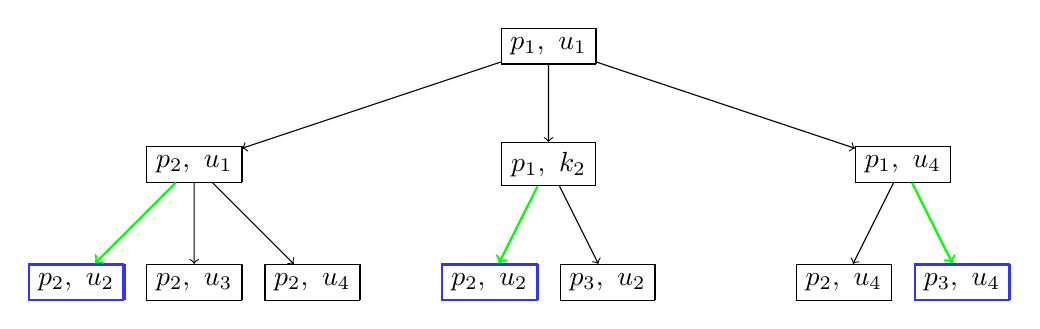
\begin{tikzpicture}
    \tikzstyle{bplus}=[rectangle split, rectangle split horizontal,rectangle split ignore empty parts,draw]
    \tikzstyle{every node}=[bplus]
    \tikzstyle{level 1}=[sibling distance=45mm]
    \tikzstyle{level 2}=[sibling distance=15mm]
    \node {$p_1,\ u_1$} [->]
      child {node {$p_2,\ u_1$ }
        child[draw=green,thick] {node[draw=blue!80, thick]{$p_2,\ u_2$}}
        child {node {$p_2,\ u_3$}}
        child {node {$p_2,\ u_4$}}    
      } 
      child {node {$p_1,\ k_2$ }
        child[draw=green,thick] {node[draw=blue!80, thick]{$p_2,\ u_2$}}
        child {node {$p_3,\ u_2$}}
      } 
      child {node {$p_1,\ u_4$ }
        child {node{$p_2,\ u_4$}}
        child[draw=green,thick] {node[draw=blue!80, thick] {$p_3,\ u_4$}}
      } 
    ;\end{tikzpicture}
\end{center}

\subsection{Secondo esempio}
Vediamo l'esempio di un gioco con due processi che dimostreremo non essere  bisimili, siano quindi:
\begin{itemize}
    \item $q_1=a\cdot b\cdot Nil+a\cdot c\cdot Nil$, nella figura a sinistra
    \item $u_1=a\cdot (\tau\cdot b\cdot Nil+\tau\cdot c\cdot Nil)$, in quella a destra
\end{itemize}
Abbiamo quindi:
\begin{figure}[H]
    \centering
    \begin{minipage}[b]{.35\textwidth}
        \centering
        \begin{tikzpicture}[shorten >=1pt,node distance=2cm,on grid,auto] 
          \node[state] (q_0) {$q_1$};  
          \node[state] (q_1) [below left =of q_0] {$q_2$};
          \node[state] (q_2) [below right =of q_0] {$q_3$};
          \node[state] (q_3) [below right =of q_1] {$Nil$};
          \path[->]
          (q_0) edge [above left] node {$a$} (q_1)
          (q_0) edge  node {$a$} (q_2)
          (q_1) edge [below left] node {$b$} (q_3)
          (q_2) edge  node {$c$} (q_3)
          ;
        \end{tikzpicture}
        \caption{$q_1$}
    \end{minipage}%
    \begin{minipage}[b]{0.35\textwidth}
        \centering
        \begin{tikzpicture}[shorten >=1pt,node distance=2cm,on grid,auto]
          \node[state] (q_0) {$u_2$};  
          \node[state] (q_1) [below left =of q_0] {$u_3$};
          \node[state] (q_2) [below right =of q_0] {$u_4$};
          \node[state] (q_3) [below right =of q_1] {$Nil$};
          \node[state] (q_4)[above =of q_0]  {$u_1$}; 
          \path[->]
          (q_0) edge [above left] node {$\tau$} (q_1)
          (q_0) edge  node {$\tau$} (q_2)
          (q_1) edge [below left] node {$b$} (q_3)
          (q_2) edge  node {$c$} (q_3)
          (q_4) edge  node {$a$} (q_0)
          ;
        \end{tikzpicture}
        \caption{$u_1$}
    \end{minipage}
\end{figure}
Vediamo quindi come si svolgono tutte le partite per $G(q_1,u_1)$.\\ 
L'attaccante esegue $u_1\stackrel{a}{\rightarrow}u_2$.Nella situazione attuale il difensore ha due scelte:
\begin{itemize}
    \item $q_1\stackrel{a}{\Rightarrow}q_2$. Sono quindi in $(q_2,u_2)$. A questo punto $u_2\stackrel{\tau}{\rightarrow}u_4$ a cui il difensore non può che rispondere con l’azione nulla, $q_2\stackrel{\tau}{\rightarrow}q_2$, perdendo in quanto $q_2\stackrel{Bis}{\not\approx} u_4$ dato che dal primo, $q_2$ posso fare solo $b$ e dal secondo, $u_4$ solo $c$
    \item $q_1\stackrel{a}{\Rightarrow}q_3$. Sono quindi in $(q_3,u_2)$. A questo punto $u_2\stackrel{\tau}{\rightarrow}u_3$ a cui il difensore non può che rispondere con l’azione nulla, $q_3\stackrel{\tau}{\rightarrow}q_3$, perdendo in quanto $q_3\stackrel{Bis}{\not\approx} u_3$ dato che dal primo, $q_3$, posso fare solo $c$ e dal secondo, $u_3$, solo $b$
  \end{itemize}
Quindi abbiamo fatto vedere, con un esempio, che ci sono dei casi di non bisimilutidine: $q_1\stackrel{Bis}{\not\approx} u_1$\\
Vediamo anche in questo caso un albero parziale, dove si vedono anche le mosse in cui l'attaccante perdeva. Sono di egual colore le configurazioni identiche e si hanno col bordo con spessore più grande le foglie (non colorate) corrispondi alle vincite del difensore, che però non ha sempre una mossa per risponde attaccante, comportando la non bisimulazione:
Le foglie colorate rappresentano parti di alberi parziali.
\begin{figure}[H]
    \centering
    \includegraphics[scale = 0.4]{IMM/albero_grosso.PNG}
\end{figure}
\section{Lezione del 11 novembre}
\subsection{Proprietà auspicate di una relazione di equivalenza}
Una proprietà di equivalenza tra processi CCS èp nella forma: $\simeq \;\subseteq  Proc_{CCS} \times  Proc_{CCS}$\\
Dati due processi $p,q\ \in Proc_{CCS}$, se $LTS(p)=LTS(q)$ (i due LTS sono isomorfi), allora $ p\simeq q$. In questo contesto si considerano solo le azioni di interazione tra componenti del sistema o in relazione con l’ambiente che si sta modellando e si astrae dagli stati.
Inoltre: 
\begin{itemize}
    \item $p\simeq q\implies Tracce(p)=Tracce(q)$, ovvero le stesse sequenze di azioni si devono poter eseguire su entrambi i processi. 
    \item $p\simeq q \implies p$ e $q$ devono avere la stessa possibilità di generare deadlock nell’interazione con l’ambiente (ovvero l’insieme dei processi con cui $p$ e $q$ possono interagire). Quindi sostituendo $p$ con $q$, qualora il primo non avesse deadlock, anche il secondo non avrà deadlock.
    \item $\simeq$ dev’essere una congruenza rispetto agli operatori del CCS, ovvero dev’essere possibile sostituire un sottoprocesso con un suo equivalente senza modificare il comportamento complessivo del sistema. 
\end{itemize}
La prima equivalenza introdotta è l'equivalenza forte rispetto alle tracce, essa si presenta nella forma $\forall p,q\in Proc_{CCS}$, e abbiamo:
\begin{itemize}
    \item $LTS(p)=LTS(q)\implies p\stackrel{T}\sim q$
    \item Si osservano solo le tracce, quindi si estrae dagli stati.
    \item $p\stackrel{T}{\sim} q \iff Tracce(p)=Tracce(q)$
    \item È una congruenza rispetto agli operatori CCS.
    \item MA questa nozione di equivalenza non garantisce di preservare il deadlock (o l’assenza di deadlock) nell’interazione con l’ambiente.
\end{itemize}
Si introduce quindi una equivalenza diversa, ovvero l'equivalenza forte rispetto alla bisimulazione o Bisimulazione forte (introdotta da Milner), in questo abbiamo che se $\forall p,q \in Proc_{CCS}$,e per la \textbf{Bisimulazione forte} abbiamo quanto segue:
\begin{itemize}
    \item $LTS(p)=LTS(q)\implies p\stackrel{Bis}\sim q$
    \item Astrae dagli stati.
    \item $p\stackrel{Bis}\sim q \implies Tracce(p)=Tracce(q)$. \\
        In altri termini si ha che $p\stackrel{Bis}\sim q \implies p\stackrel{T}\sim q$ e quindi $\stackrel{Bis}{\sim} \; \subseteq \; \stackrel{T}{\sim}$, cioè non si possono avere processi bisimili che non abbiano le stesse tracce.
    \item il vantaggio principale è che la bisimulazione, a differenza delle tracce, preserva il deadlock o l’assenza di deadlock nell’interazione con l’ambiente.
    \item È una congruenza rispetto agli operatori del CCS. 
    \item Ma  $\stackrel{Bis}\sim$ è troppo restrittiva infatti (come anche $\stackrel{T}\sim$)  non astrae rispetto alle azioni non osservabili, di  sincronizzazione, $\tau$. \\ Infatti per esempio, $a\cdot b\cdot Nil \stackrel{Bis}{\not\sim} a\cdot \tau\cdot b\cdot Nil$. 
\end{itemize}
È stata quindi introdotta la regola di transizione debole $(\stackrel{a}{\Rightarrow})$, l’equivalenza debole rispetto alle tracce $(\stackrel{T}{\approx})$ e la bisimulazione debole $(\stackrel{Bis}{\approx})$.\\
\subsection{Nozioni sulle equivalenze}
\subsubsection{ Equivalenza rispetto alle tracce \texorpdfstring{($\stackrel{T}\sim$ e $\stackrel{T}{\approx}$)}{}}
L’equivalenza forte rispetto alle tracce è più restrittiva rispetto all’equivalenza debole rispetto alle tracce: $p \stackrel{T}\sim q \implies p \stackrel{T}{\approx} q$ e quindi $\stackrel{T}\sim \; \subseteq \;  \stackrel{T}{\approx}$.
Anche Equivalenza debole rispetto alle tracce debole $\forall p,q\in Proc_{CCS}$
\begin{itemize}
    \item $LTS(p)=LTS(q)\implies p \stackrel{T}{\approx} q$
    \item Astrae dagli stati.
    \item È una congruenza rispetto agli operatori del CCS.
    \item MA non garantisce di preservare il deadlock o l’assenza di deadlock nell’interazione con l’ambiente.
\end{itemize}

\subsubsection{Bisimulazione forte e debole \texorpdfstring{$\stackrel{Bis}{\sim}$ e  $\stackrel{Bis}{\approx}$}{}}
La bisimulazione forte è più restrittiva della bisimulazione debole: $p \stackrel{Bis}\sim q \implies p \stackrel{Bis}{\approx} q$ e quindi $\stackrel{Bis}\sim \; \subseteq \;  \stackrel{Bis}{\approx}$. \\
Inoltre La bisimulazione forte (debole) è più restrittiva dell’equivalenza forte (debole) rispetto alle tracce, infatti si ha:
$p \stackrel{Bis}\sim q \implies p \stackrel{T}\sim q$ e $p \stackrel{Bis}\approx q\implies p \stackrel{T}\approx q$, quindi si ha che $\stackrel{Bis}\sim \; \subseteq \; \stackrel{T}\sim$ e $\stackrel{Bis}\approx \; \subseteq \; \stackrel{T}\approx$.
\subsubsection{Processi deterministici ed equivalenze}
Un processo $p\in Proc_{CCS}$ è un processo deterministico $$\iff \forall x\in Act = A \cup \bar{A} \cup \{\tau\}, \mbox{ se } p\stackrel{x}{\rightarrow}p'\mbox{ e }p\stackrel{x}{\rightarrow}p''\mbox{ allora }p'=p''$$
Quindi se si può passare a $p'$ o $p''$ con la stessa azione allora necessariamente questi due processi coincidono. Ma cosa succede se io confronto tra loro solamente processi deterministici? Quello che possiamo dire è che se io confronto processi deterministici con l'equivalenza rispetto alle tracce e risultano equivalenti risptto alle tracce, allora sono anche equivalenti anche rispetto alla bisimulazione. Questo è descritto nella seguetne preposizione in modo formale:\\
\textbf{Proposizione}
Siano $p,q\in Proc_{CCS}$. 
Se $p$ e $q$ sono deterministici e $p \stackrel{T}{\sim} q$ (quindi anche $p \stackrel{T}{\approx} q$), allora $p \stackrel{Bis}{\sim} q$ (quindi anche $p \stackrel{Bis}{\approx} q$).

\subsubsection{Proprietà della bisimulazione debole \texorpdfstring{$\stackrel{Bis}{\approx}$}{}}
\begin{itemize}
    \item Essendo l’unione di tutte le relazioni di bisimulazione, è la più grande relazione di bisimulazione debole ed è una relazione di equivalenza, essendo     riflessiva, simmetrica e transitiva.
    \item Come per la bisimulazione forte, preserva la possibilità di generare o meno deadlock nell’interazione con l’ambiente.
    Quindi sostituendo un processo che (non) genera deadlock con un suo bisimile, si ha che anche il nuovo sistema (non) andrà in deadlock; ciò non è vero per l’equivalenza sulle tracce.
    \item A differenza della bisimulazione forte, astrae da azioni non osservabili ($\tau$) e da cicli inosservabili ($\tau$ loop). 
    In caso di ciclo infinito di $\tau$, si parla di divergenza. Ad esempio, dati due processi $Nil$ e $p=\tau\cdot p$ ($p$ è un processo infinito di sole $\tau$, una divergenza), si ha che $Nil \stackrel{Bis}{\approx} p$.
\end{itemize}

Una relazione di equivalenza $R\subseteq Proc_{CCS}\times Proc_{CCS}$ è una congruenza se $\forall$ contesto CCS $C[$ \textbullet $ ]$ (con una certa variabile \textbullet), allora succede che se $p\ R\ q \implies C[p]\; R \;C[q]$ con $p,q\in Proc_{CCS}$. Quindi comunque si prenda una specifica CCS si devono poter sostituire a piacere i due processi. Da questo deriviamo un teorema che dice:
\begin{teorema}{Teorema}{}
\par
    $\forall\,p,q\in Proc_{CCS}$ se $p \stackrel{Bis}{\approx} q$, allora:
    \begin{itemize}
        \item $\forall\, \alpha \in Act=A\cup\bar{A}\cup\{\tau\}$,	$\alpha \cdot p \stackrel{Bis}{\approx} \alpha \cdot q$
        \item  $\forall\,r\in Proc_{CCS}$,	$p|r \stackrel{Bis}{\approx} q|r \; \land \; r|p \stackrel{Bis}{\approx} r|q$
        \item $\forall\,f$ funzione di rietichettatura,	$p[f] \stackrel{Bis}{\approx} q[f]$\\
            Le funzioni di rietichettatura preservano nomi, co-nomi e $\tau$(l’immagine di un co-nome è uguale al co-nome dell’immagine) .
        \item $p\setminus_L \stackrel{Bis}{\approx} q \setminus_L$,	$\forall\,L\subseteq A$\\
            La restrizione rispetto a $L$ comporta che il processo può eseguire le azioni in $L$ solo se sono sincronizzazioni interne. Non può essere sincoronizzato con l'ambiente.
    \end{itemize}
\end{teorema}
A differenza della bisimulazione forte, la bisimulazione debole non è una congruenza rispetto agli operatori del CCS, in quanto non è una congruenza rispetto all’operatore scelta ($+$). Inoltre, la bisimulazione debole non è una congruenza per la ricorsione.\\

Si vuole trovare una relazione di congruenza, definita come relazione binaria tra processi CCS, che sia la più grande relazione contenuta nella bisimulazione e che sia una congruenza rispetto a tutti gli operatori: $$\stackrel{C}{\approx} \; \subseteq \; \stackrel{Bis}{\approx} \; \subseteq Proc_{CCS}\times Proc_{CCS}$$

Per il CCS puro senza ricorsione, Milner ha introdotto un insieme finito di assiomi che possono essere visti come regole di riscrittura che preservano la congruenza all’osservazione, che è la più grande congruenza contenuta nella bisimulazione. 
Questo insieme di assiomi è quindi un insieme finito per il quale, presi due processi $p,q\in Proc_{CCS}$, se si riesce (utilizzando gli assiomi) a trasformare l’uno nell’altro, allora si ha che $p$ e $q$ non sono solo bisimili ma anche congruenti (potendo quindi sostituire l’uno con l’altro in qualsiasi contesto che non includa la ricorsione). \\
Questo insieme di assiomi, detto $Ax$, è:
\begin{itemize}
    \item corretto: se utilizzando l’insieme di assiomi si deduce che $p=q$ allora $p$ è congruente a $q$ rispetto alla nozione di congruenza $\stackrel{C}{\approx}$: $Ax\vdash p=q\implies p \stackrel{C}{\approx} q$
    \item completo: presi due processi che sono congruenti secondo la nozione di congruenza $\stackrel{C}{\approx}$, allora sicuramente l’insieme di assiomi è completo in quanto permette di trascrivere $p$ in $q$: $p \stackrel{C}{\approx} q\implies Ax\vdash p=q$
    \end{itemize}
    Assiomi della relazione di congruenza $\stackrel{C}{\approx}$:
    \begin{itemize}
    \item associatività di scelta e composizione parallela:	$p+(q+r) \stackrel{C}{\approx} (p+q)+r$	e	$p|(q|r) \stackrel{C}{\approx} (p|q)|r$
    \item commutatività di scelta e composizione parallela:	$p+q \stackrel{C}{\approx} q+p$	e	$p|q \stackrel{C}{\approx} q|p$
    \item assorbimento riguardo la scelta:	$p+p \stackrel{C}{\approx} p$ \\
        Non si ha l’assorbimento riguardo la composizione parallela, infatti $p|p \stackrel{C}{\not \approx} p$
    \item assorbimento del $Nil$ riguardo la scelta e la composizione parallela:	$p+Nil \stackrel{C}{\approx} p$	e	$p|Nil \stackrel{C}{\approx} p$
    \item assioma che risolve il problema di avere una scelta con un una $\tau$ iniziale nella sequenza ($\tau$ non può essere eliminata): $p+\tau\cdot p \stackrel{C}{\approx} \tau\cdot p$
    \item assioma che  tratta le $\tau$ interne alla sequenza (possono essere eliminate):	$\mu\cdot \tau\cdot p \stackrel{C}{\approx} \mu\cdot p$, $\forall\,\mu\in Act$
    \item $\mu\cdot(p+\tau\cdot q) \stackrel{C}{\approx} \mu\cdot(p+\tau\cdot q)+\mu\cdot q$
    \item se i due processi $p$ e $q$ sono delle somme, ovvero: $\displaystyle p=\sum_i a_i\cdot p_i, \; a\in Act$ e $\displaystyle q=\sum_j b_j\cdot q_j,\; b\in Act$ si hanno i seguenti ulteriori assiomi:
        \begin{itemize}
            \item teorema di espansione di Milner:	$p|q \stackrel{C}{\approx} \displaystyle \sum_i \alpha_i\cdot (p_i|q)+\sum_j \beta_j \cdot (p|q_j) + \sum_{\alpha_i=\bar{\beta_j}} \tau \cdot(p_i|q_j)$\\
                Se $a_i$ e $b_j$ sono l’uno il complemento dell’altro allora si possono sincronizzare su di essi i processi, che diventano una $\tau$ e proseguendo con $p_i|q_j$.
            \item $\displaystyle p[f] \stackrel{C}{\approx} \sum_if(a_i)\cdot(p_i[f]), \; \forall\,f$ funzione di etichettatura\\
                Rietichettare tutto il processo $p$ corrisponde al fatto di ottenere congruo il processo, che ottengo etichettando ogni i-sima azione delle componenti che sono in alternativa, concatenato con il processo relativo rietichettato con $f$.
            \item $\displaystyle p_{\backslash L} \stackrel{C}{\approx} \sum_{a_i,\overline{a_i}\not\in L}a_i\cdot(p_{i\backslash L}),\,\,\,\forall\,L\subseteq A$\\
                Si considerano solo le azioni per le quali non si ha alcuna restrizione.
        \end{itemize}
\end{itemize}
Per cui la bisimulazione risulta tale per cui se si utilizza $\stackrel{C}{\approx}$ si può modellare un sistema a passi successivi sapendo che è possibile sostituire un sottoprocesso con un altro ottenendo ancora un sistema bisimile al precedente.
\section{Lezione del 20 novembre}
Le reti di Petri sono state introdotte da Carl Adam Petri nel 1962 con l’obiettivo di descrivere il flusso di informazione tra le componenti di un sistema complesso.

Nei sistemi distribuiti lo stato globale non è osservabile; quindi la simulazione sequenziale non deterministica (semantica a interleaving) dei sistemi distribuiti è una forzatura, non rappresenta le caratteristiche reali del comportamento. La soluzione di Petri consiste nell’utilizzo delle reti di Petri per i sistemi elementari. In questi se devo specificare il \textbf{produttore-consumatore}, vado a specificare il mio sistema a livello di: Quali sono gli stati locali del sistema e quali sono gli eventi, in questo caso dell'ambiente.

Una transizione, nel modello dei Sistemi di Transizioni Etichettati, prende uno stato globale e lo trasforma in un altro stato globale. Nelle reti di Petri, invece, la transizione è locale che dipende da alcune precondizioni e produce postcondizioni.

Lo \textbf{stato} viene definito da una collezione di stati locali, ovvero condizioni vere. Gli stati locali sono rappresentati da cerchi e rappresentano condizioni booleane (vere se presentano un pallino, false altrimenti).\\

Abbiamo inoltre gli eventi, ovvero le nostre transizione locali, rappresentata con quadrati. Gli stati locali determinano quali eventi sono \textbf{abilitati}, ovvero possono occorrere. \\
Due eventi occorrono in modo \textbf{concorrente} se vengono abilitati contemporaneamente.
\subsection{Le reti elementari}
Una rete $N = (B,E,F)$ è una rete, questa possiamo rappresentarla attraverso un grafo bipartito, tale che:
\begin{itemize}
    \item $B$: insieme finito di condizioni (stati locali, proprietà booleane) rappresentate da cerchi (\textbigcircle).
    \item $E$: insieme finito di eventi (trasformazioni locali di stato, transizioni locali) rappresentati da quadrati ($\square$).
    \item $B \cap E = \varnothing$ e $B \cup E \neq \varnothing$ ($B$ e $E$ sono insiemi disgiunti e non vuoti)
    \item $F \subseteq (B \times E) \cup (E \times B)$: relazione di flusso, rappresentata da una freccia, tale che:\\
        $dom(F) \cup ran(F) = B \cup E$, ovvero non ci sono elementi isolati.
        Una condizione isolata non cambia mai di valore e quindi non è osservabile (in quanto la si osserverebbe solo nel momento in cui dovesse cambiar valore), pertanto non la si modella perché non ha influenza sul sistema. 
        Un evento isolato non ha influenza su alcuna condizione, non ha pertanto né precondizioni né postcondizioni, e non è rilevabile, pertanto non lo si modella. 
\end{itemize}

Sia $x \in B \cup E = X$, possiamo identificare :
\begin{enumerate}
    \item \textbullet $ x = \{y \in X \; | \; (y,x) \in F\}$ come pre-elementi di $x$ (precondizioni o pre-eventi)
    \item $x$\textbullet$= \{y \in X \; | \; (x,y) \in F\}$	come post-elementi di $x$ (postcondizioni o post-eventi)
\end{enumerate}

Il concetto di pre e post lo posso estendere alle sotto-condizioni/eventi. E le possiamo ottenere l'insieme delle precondzioni \textbullet$A$eseguendo eseguendo l'unione di tutti i \textbullet$X$, discorso analogo per le post condizioni. Condizioni ed eventi sono nozioni duali. 

Sia $A \subseteq B \cup E$, allora \textbullet$A = \displaystyle \bigcup_{x \in A} $\textbullet$x$ e $A $\textbullet$ = \displaystyle \bigcup_{x \in A} x$\textbullet\\

La rete $N = (B, E, F)$ descrive la struttura del sistema, ovvero le relazioni tra le condizioni e gli eventi. 
Il comportamento è definito attraverso le nozioni di caso e di regola di scatto o di transizione.\\

Un caso,configurazione oppure stato globale è un insieme di condizioni $c \subset B$ che rappresentano l’insieme di condizioni vere di una certa configurazione del sistema, ovvero un insieme di stati locali che collettivamente individuano lo stato globale del sistema. \
Abbiamo quindi una condizione falsa \textbigcircle  e una condizione vera $\Large \astrosun$\\

Ho una rete e un sottoinsieme di condizioni, che in una certa condizione presumo siano vere. Devo quindi sapere dire quando un evento, data una certa condizione, può occorrere (essere abilitato), per farlo utilizzo una\textbf{ regola di scatto} o \textbf{regola di transizione} \\

Sia $N = (B, E, F)$ una rete elementare e $c \subset B$.
L’evento $e \in E$ è abilitato (può occorrere) in $c$, denotato con $c[e >$ $\iff $\textbullet$ e \subseteq c \; \land \; \{e $\textbullet$\} \cap c = \varnothing$ (quindi se le precondizioni sono vere e le postcondizioni sono false).\\
Se $c$ in $c[e >$ non rappresenta solo le precondizioni dell’evento $e$, ma tutte le condizioni vere in quel momento; quindi le precondizioni di $e$ sono un sottoinsieme di $c$.\\ 
Se $c[e >$, allora, quando $e$ occorre in $c$, genera un nuovo caso $c'$. Ricordando che $c$ rappresentava un insieme, otteniamo che $c'$, in seguito a $c[e > c'$, sarà così composto: $c' = (c \setminus \{$\textbullet$ e\}) \cup \{e $\textbullet$\}$. In poche parole tolgo dall'insieme le pre condizioni e unisco le postcondizioni.\\
Due eventi non interferiscono uno con l’altro (sono indipendenti) se hanno pre e post condizioni disgiunte.

\subsection{Principio di estensionalità}
Principio di estensionalità (il cambiamento di stato è locale): un evento è completamento caratterizzato dai cambiamenti che produce negli stati locali e che sono indipendenti dalla particolare configurazione in cui l’evento occorre.

Sia $N = (B,E,F)$ \textbf{una rete elementare}:
\begin{itemize}
    \item $N$ è semplice $\iff \forall x,y \in B \cup E, \;  $\textbullet$ x = $\textbullet$ y \; \land \; x $\textbullet$ = y $\textbullet$ \implies x = y$\\
        Essendo che le due condizioni $x$ e $y$ cambiano valore di verità in maniera sincronizzata, (altrimenti l’evento per cui sono precondizioni o postcondizioni non si potrà mai verificare), non ha senso separarle in due variabili distinte.
    \item $N$ è pura $\iff \forall e \in E, \; $\textbullet$ e \cap e $\textbullet$ = \varnothing$
        Nel caso in cui \textbullet$ e \cap e $\textbullet$ \neq \varnothing$ (rete non pura), $e$ non occorre mai quindi non viene modellato. 
\end{itemize}
  Nelle reti 1-safe (non elementari), il caso \textbullet$ e \cap e $\textbullet$ \neq \varnothing$ viene visto come un modo più sintetico per rappresentare un’ulteriore condizione che si frammezza tra \textbullet$ e$ e $e $\textbullet.
\section{Lezione del 23 novembre}
Sia $N = (B, E , F)$ una rete elementare, $U \subseteq E$ e $c, c_1, c_2 \subseteq B$. Diciamo che: 
\begin{itemize}
    \item $U$ è un \textbf{insieme di eventi indipendenti }$\iff \forall e_1,e_2 \in U:\ e_1 \neq e_2 \Rightarrow (^\bullet e_1 \cup e_1 ^\bullet) \cap (^\bullet e_2 \cup e_2 ^\bullet) = \emptyset$ 
    \item $U$ è \textbf{un passo abilitato } (insieme di eventi concorrenti) in $c(c[U >)$ se e solo se, $U$ è un insieme di elementi tra loro indipendenti e ogni elemento è abilitato:
    $\forall e \in U:\ c[e>$
    \item $U$ è in \textbf{passo da} $c_1$ a $c_2$, $(c_1[ U > c_2)$ se e solo se l'insieme $U$ è abilitato in $c_1$ e $c_2$ è caso in cui, prendendo $c_1$ togliendo tutt le precondizioni e aggiungendo tutte le post condizioni dell'insieme.\\ $c_1[> U \land c_2 = (c_1 - ^\bullet U) \cup U ^\bullet$
\end{itemize}
{\centering
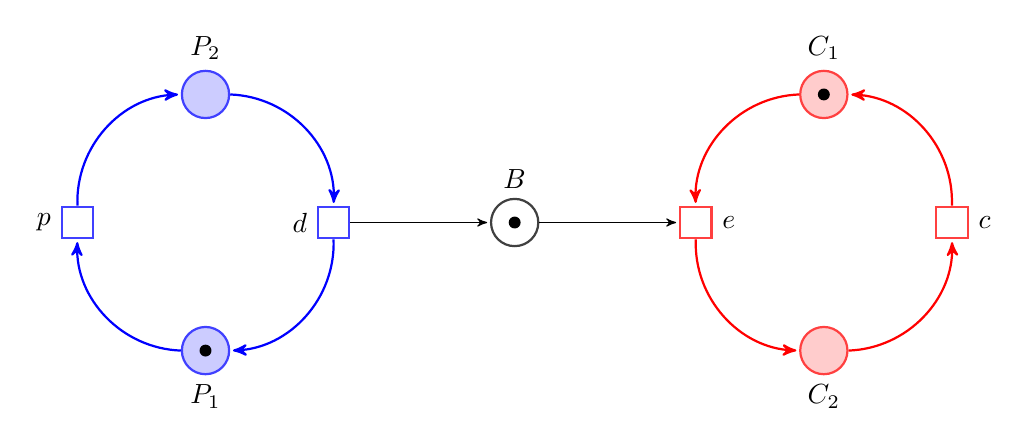
\begin{tikzpicture}[node distance=2.3cm,>=stealth',bend angle=45,auto]

  \tikzstyle{place}=[circle,thick,draw=blue!75,fill=blue!20,minimum size=6mm]
  \tikzstyle{transition}=[rectangle,thick,draw=blue!75,minimum size=4mm]

    \node [place, tokens=1] (p1)    [label=below:$P_1$]         {}; %P1
    \node [transition] (p) [above left of=p1, label=left:$p$] {}                   %this is new p
        edge [pre ,bend right, blue,thick]  (p1);
    \node [place] (c1) [above right of=p, label=above:$P_2$] {};      %P2
    \node [transition] (p) [above left of=p1] {} %this is new p
        edge [post ,bend left,blue,thick]  (c1);
    \node [transition] (d) [above right of=p1,label=left:$d$] {} %this is d
        edge [pre ,bend right,blue,thick]  (c1)
        edge [post, bend left,blue,thick]  (p1);
        
    \node [place,tokens=1, fill=white,draw=black!75] (b) [right of=d, label=above:$B$] {};
    \node [transition] (d) [above right of=p1] {} %this is d
        edge [post]  (b);
    \node [transition] (e) [right of=b] {} %this is d
        edge [pre]  (b);
    \node[place, tokens=1,fill=red!20,draw=red!75] (c1) [above right of=e, label=above:$C_1$] {};
    \node[place, fill=red!20,draw=red!75] (c2) [below right of=e,label=below:$C_2$ ] {};
    \node [transition,fill=white,draw=red!75] (e) [right of=b,label=right:$e$] {} %this is d
        edge [pre, bend left, red, thick]  (c1)
        edge [post, bend right,red, thick]  (c2);
        
    \node [transition,fill=white,draw=red!75] (c) [above right of=c2,label=right:$c$] {} %this is d
        edge [post, bend right, red, thick]  (c1)
        edge [pre, bend left,red, thick]  (c2);
\end{tikzpicture}
\par}

Da questa figura possiamo capire facilmente le seguenti cose:
\begin{itemize}
    \item $\{p,e\},\{p,c\},\{d,c\}$ sono esempi di insiemi di eventi indipendenti
    \item $\{p,e\}$ è un passo abilitato di $\{P_1,B,C_1\}$
    \item $\{P_1,B,C_1\}[\{p,e\} >\{P_2,C_2\} $
\end{itemize}

Un \textbf{sistema elementare} $\Sigma = (B,E,F, c_{in})$ è definito da una rete $N = (B, E , F)$ e da $c_{in} \subseteq B$ che rappresenta un caso iniziale della rete. \\
L'insieme dei \textbf{casi raggiungibili} ($C_{\Sigma}$) del sistema elementare $\Sigma = (B,E,F, c_{in})$ è il più piccolo sottoinsieme di $2^B$ tale che:
\begin{itemize}
    \item il caso iniziale appartiene all'insieme dei casi raggiungibili: $c_{in} \in C_{\Sigma}$.
    \item se $c$ è un caso raggiungibile, $U$ è un insieme di eventi indipendenti abilitati in $c$,e nel momento in cui $U$ è abilitato in c questo mi porta in $c'$ allora anche $c'$ è raggiungibile: $c \in C_{\Sigma}$ e $U \subseteq E$, $c' \subseteq B$ sono tali che se $c[U > c' \implies c' \in C_{\Sigma}$. 
\end{itemize}
In questo modo ho definiti tutti i casi raggiungibili $C_{\Sigma}$ partendo da $c_{in}$.\\

Possiamo definire, dato un sistema, anche l'insieme dei possibili passi abilitati in un qualche caso raggiungibile. \\ Diremo che $U_{\Sigma}$ è l'insieme dei passi di $\Sigma : \{U \subseteq E \ | \ \exists c,c'\in C_{\Sigma}: \ c[U >c' \}$

\subsection{Il comportamento dei sistemi elementari}
Sia $\Sigma = (B,E,F, c_{in})$ un sistema elementare,  $c_{i} \in C_{\Sigma}$. e  $e_{i} \in E$.
\begin{itemize}
    \item si vanno a considerare tutte le possibili sequenze di eventi partendo dal caso iniziale. Quindi si studia il \textbf{comportamento sequenziale}, riotteniamo la semantica di interleaving (simulazione sequenziale non deterministica), per esempio osserviamo una sequenza ottenuta da un sistema finito, dove quindi non si presentano loop (ci sono due possibili notazioni che possiamo utilizzare):
    $c_{in} [e_1  > c_1[e_2 > \dots [e_n > c_n$ oppure $c_{in} [e_1\ e_2 \dots e_n> c_n$
    \item si possono descrivere anche i comportamenti non sequenziali, descrivendo quindi le sequenze di passi, tenendo conto che $U_i$ rappresentano semplicemente sotto insieme di eventi che sono indipendenti e possono scattare in sequenza:  
    $c_{in} [U_1  > c_1[U_2 > \dots [U_n > c_n$ oppure $c_{in} [U_1\ U_2 \dots U_n> c_n$
    \item in fine abbiamo il comportamento non sequenziale, o processi non sequenziali, che danno origine al \textit{partial order semantics}, andando a considerare l'ordine parziale che esiste tra gli eventi.
\end{itemize}
Si ricorda che si possono utilizzare sequenze sia finite che infinite di passi o eventi. 
{\centering
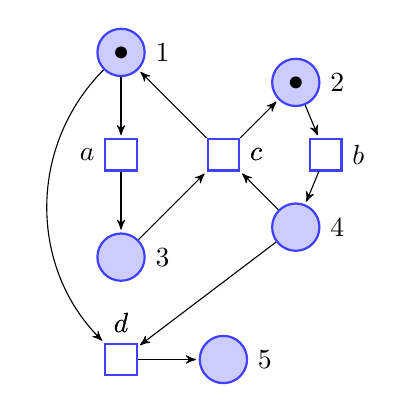
\begin{tikzpicture}[node distance=1.3cm,>=stealth',bend angle=45,auto]
  \tikzstyle{place}=[circle,thick,draw=blue!75,fill=blue!20,minimum size=6mm]
  \tikzstyle{transition}=[rectangle,thick,draw=blue!75,minimum size=4mm]

    \node [place, tokens=1] (uno)   [label=right:$1$]         {}; %P1
    \node [transition] (a) [below of =uno] {}
        edge [pre]  (uno);
    \node [place ] (tre)[label=right:$3$]  [below of =a]       {}; %P1
    \node [transition] (a) [below of =uno,label=left:$a$] {}
        edge [post]  (tre);
    \node [transition] (c) [right of =a, label=right:$c$] {}
        edge [post]  (uno)
        edge [pre] (tre);
    \node [place, tokens=1] (due)  [above right of = c,label=right:$2$]         {}; %P1
    \node [place]       (quattro)  [below right of = c,label=right:$4$]         {}; %P1    
    \node [transition]        (c)  [right of =a,label=right:$c$] {}
        edge [post]  (due)
        edge [pre] (quattro);
     \node [transition] (b) [right of = c,label=right:$b$] {}
        edge [post]  (quattro)
        edge [pre] (due);
    \node [transition] (d) [below of = tre,label=above:$d$] {}
        edge [pre]  (quattro)
        edge [pre, bend left] (uno);
    \node [place]       (cinque)  [right of = d,label=right:$5$]         {}; %P1    
    \node [transition] (e) [below of = tre,label=above:$d$] {}
        edge [post]  (cinque);
\end{tikzpicture}
\par}

In questo caso abbiamo che una possibile sequenza di occorrenze di eventi è data da:
\begin{itemize}
    \item $\{1,2\}[a> \{3,2\}[b > \{3,4\}[c>\{1,2\}[b> \{1,4\}[d>\{5\}$
\end{itemize}
Invece una possibile sequenza di passi è data da:
\begin{itemize}
    \item $\{1,2\}[\{a,b\} > \{3,4\}[\{c\} > \{1,2\}[\{b\}> \{1,4\}$
\end{itemize}
Invece una processo non sequenziale di $\Sigma$:
\begin{figure}[H]
    \centering
    \includegraphics[scale = .5]{IMM/seq_immag_1.PNG}
\end{figure}

\subsection{Grafi dei casi raggiungibili}
Il comportamento di un sistema elementare $\Sigma = (B,E,F, c_{in})$ può essere rappresentato dal suo grafo dei casi. \\
Il \textbf{grafo dei casi} di $\Sigma$ è il sistema di transizioni etichettato $GG_{\Sigma}  = (C_{\Sigma},U_{\Sigma}, A, c_{in})$ dove:
\begin{itemize}
    \item $C_{\Sigma}$ è l'insieme dei nodi del grafo (gli stati globali)
    \item $U_{\Sigma}$ è l’alfabeto
    \item $A$ è l'insieme di archi etichettati 
    \[A = \{(c, U, c')| c, c' \in C_{\Sigma}, U \in U_{\Sigma}, c[U > c' \}\]
    \begin{figure}[H]
        \centering
    \includegraphics[scale = .5]{IMM/seq_immag_2.PNG}
\end{figure}
\end{itemize}


\subsection{Diamond Property}
Dato un sistema elementare $\Sigma = (B,E,F;c_{in})$ e il suo grafo dei casi $CG_\Sigma=(C_\Sigma, U_\Sigma, A, c_{in})$ si ha che il grafo soddisfa una particolare proprietà, detta \textbf{diamond property}, tipica solo dei sistemi elementari.
La \textbf{diamond property} stabilisce una proprietà della struttura del grafo della rete elementare, ovvero, dati $U_1,U_2\in U_\Sigma$ tali che:$U_1\cap U_2=\emptyset$,$U_1\neq\emptyset$ e  $U_2\neq\emptyset$ e dati $c_i\in C_\Sigma$ allora vale, per esempio:
\begin{figure}[H]
    \centering
    \includegraphics[scale = 0.6]{IMM/diamond.jpg}
    \label{fig:dia}
\end{figure}
ovvero se posso rilevare come sottografo una struttura come quella a sinistra nell'immagine allora sicuramente tale sottografo contiene anche gli archi per ottenere l'immagine di destra. Si possono fare delle prove:
\begin{enumerate}
  \item \textbf{prima prova:}\\
  Dimostriamo che possiamo passare all'immagine di destra da quella di sinistra aggiungendo i due archi mancanti.\\ Diciamo che $U_i$ è un singolo evento $e_i$, con $i=1,2$. Siano inoltre $c_1,c_2\in C_\Sigma$, ovvero sono casi raggiungibili, ed $e_1,e_2\in E$ tali che $c_1 [e_1 > c_2 [e_2 > \mbox{ e } c_1 [e_2 >$. Si vuole dimostrare che: \[(^\bullet e_1\cup e_1^\bullet)\cap(^\bullet e_2\cup e_2^\bullet)=\emptyset\] ovvero che i due eventi sono indipendenti, che sono entrambi abilitati e che sono eseguibili in qualsiasi ordine. 
  Da $c_1 [e_1 > \mbox{ e }c_1 [e_2 >$ segue che:  $^\bullet e_1\cap e_2^\bullet=\emptyset$ e $^\bullet e_2\cap e_1^\bullet=\emptyset$. Infatti se $e_1$ e $e_2$ sono entrambi abilitati in $c_1$, le loro pre-condizioni sono vere e le post-condizioni false, e quindi non è possibile che una condizione sia contemporaneamente precondizione di $e_1$ (vera) e anche postcondizione di $e_2$ (falsa), e viceversa. Quindi le precondizioni di un evento sono disgiunte dalle postcondizioni dell'altro.\\ Inoltre dal fatto che ho $c_1 [e_1 > c_2 [e_2$, ovvero che da $c_1$ è abilitato $e_1$ e che dopo lo scatto di $e_1$ è ancora abilitato $e_2$ possiamo dire che: $e_1^\bullet\cap e_2^\bullet=\emptyset$ e $^\bullet e_1\cap\, ^\bullet e_2=\emptyset$  in $c_2$, infatti, le pre-condizioni di $e_1$ sono false mentre le precondizioni di $e_2$ sono vere e quindi $e_1$ e $e_2$ non possono avere precondizioni in comune; inoltre sempre in $c_2$ le postcondizioni di $e_1$ sono vere, mentre quelle di $e_2$ sono false, e quindi $e_1$ e $e_2$ non possono avere post-condizioni in comune. Quindi le precondizioni dei due eventi sono disgiunte, come del resto anche le postcondizioni, in quanto i due eventi sono sequenziali.\\ Si è quindi dimostrato che i due eventi hanno precondizioni e postcondizioni completamente disgiunte e quindi la tesi è verificata
  \item \textbf{seconda prova:}\\
  Analizzando la situazione:
  \begin{figure}[H]
    \centering
    \includegraphics[scale = 0.45]{IMM/diam2.jpg}
  \end{figure}
  Si supponga che $U_1\cup U_2\in U_\Sigma$ e che si abbiano:
  \begin{itemize}
    \item $U_1\cap U_2=\emptyset$, ovvero sono disgiunti
    \item $U_1\neq\emptyset$
    \item $U_2\neq\emptyset$
  \end{itemize}
  allora se $c_1[(U_1\cup U_2)>c_3$, quindi è abilitato il passo $U_1\cup U_2$ in $c_1$, sicuramente si ha che sono abilitati anche i singoli passi:
  \begin{itemize}
    \item $c_1[U_1>$
    \item $c_1[U_2>$
  \end{itemize}
resta da dimostrare che dopo lo scatto di $U_1$ è ancora abilitato $U_2$ in $c_2$. Ma se $U_1\cup U_2$ è un passo abilitato significa che posso eseguirli in qualsiasi ordine, quindi anche prima $U_1$ e poi $U_2$, e questo comporta sicuramente che $U_2$ è abilitato e che porta a $c_3$. Analogamente invertendo $U_1$ e $U_2$, formalmente:
  \begin{itemize}
    \item $c_1[U_1>c_2[U_2>c_3$
    \item $c_1[U_2>c_4[U_1>c_3$
  \end{itemize}
  Si dimostra così che l'immagine di sinistra comporta quella di destra.
\end{enumerate}

\subsection{Grafo dei casi sequenziale}
Un \textbf{grafo dei casi sequenziale} del sistema elementare $\Sigma=(B,E,F;c_{in})$ è una quadrupla in $SCG_\Sigma=(C_\Sigma,E,A,c_{in})$ dove le etichette sono i singoli eventi (mentre il resto rimane definito come nel grafo dei casi raggiungibili). Formalmente si ha quindi che:
$A=\{(c,e,c')|\,c,c'\in C_\Sigma,\,e\in E:\, c[e>c'\}$
\begin{figure}[H]
    \centering
    \includegraphics[scale = 0.6]{IMM/seq3.jpg}
\end{figure}
Per la \textbf{diamond property}, nei sistemi elementari il grafo dei casi e il grafo dei casi sequenziale sono \textbf{sintatticamente equivalenti} (possono essere ricavati l’uno dall’altro). Questo implica il fatto che due sistemi elementari hanno grafi dei casi isomorfi se e solo se hanno grafi dei casi sequenziale isomorfi.

\subsection{Isomorfismo tra Sistemi di Transizione Etichettati}
Siano dati due sistemi di transizione etichettati:  $A_1 = (S_1,E_1,T_1,s_{01})$ e $A_2 = (S_2 , E_2 , T_2 , s_{02})$ e siano date due \textbf{mappe biunivoche}:
\begin{enumerate}
    \item $\alpha:S_1\to S_2$, ovvero che passa dagli stati del primo sistema a quelli del secondo
    \item $\beta:E_1\to E_2$, ovvero che passa dagli eventi del primo sistema a quelli del secondo
\end{enumerate}
  allora: \[\langle \alpha,\beta\rangle:A_1= (S_1 , E_1 , T_1 ,s_{01})\to A_2 = (S_2 ,E_2 , T_2 , s_{02})\] è un \textbf{isomorfismo} sse:
\begin{itemize}
    \item $\alpha(s_{01})=s_{02}$, ovvero l'immagine dello stato iniziale del primo sistema coincide con lo stato iniziale del secondo
    \item $\forall s,s'\in S_1,\forall e\in E_1:\,(s,e,s')\in T_1 \Leftrightarrow (\alpha(s),\beta(e),\alpha(s'))\in T_2$ ovvero per ogni coppia di stati del primo sistema, tra cui esiste un arco etichettato $e$, vale che esiste un arco, etichettato con l'immagine di $e$, nel secondo sistema che va dall'immagine del primo stato (considerato del primo sistema) all'immagine del secondo stato (considerato del secondo sistema), e viceversa
  \end{itemize}
  
Due sistemi $\Sigma_1$ e $\Sigma_2$ sono equivalenti  sse hanno grafi dei casi sequenziali, e quindi di conseguenza anche grafi dei casi, \emph{isomorfi}.\\

\subsection{Il Problema della Sintesi}
Dato un sistema di transizioni etichettato $A=(S,E,T,s_0)$, con: 
\begin{itemize}
  \item $S$ insieme degli stati
  \item $E$ insieme delle etichette, ovvero degli eventi
  \item $T$ insieme delle transizioni
  \item $s_0$ stato iniziale
\end{itemize}
ci si propone di stabilire se esiste un sistema elementare $\Sigma=(B,E,F;c_{in})$, tale che l'insieme degli eventi del sistema corrisponda con l'insieme delle etichette di $A$ e tale che il suo grafo dei casi $SCG_\Sigma$ sia isomorfo ad $A$. In caso affermativo costruire $\Sigma$.\\ 

Il problema è stato risolto mediante la cosiddetta \textbf{teoria delle regioni}. Una \textbf{regione} comunque è un particolare sottoinsiemi di stati, legati tramite una certa condizione. Si può però dire che $A$ dovrà soddisfare la diamond property, in quanto altrimenti non sarebbe un sistema di transizioni che potrebbe corrispondere al comportamento di un sistema elementare.

\subsubsection{Contatto}
Sia $\Sigma = (B,E,F;c_{in})$ un sistema elementare e siano $e\in E$ un evento e $c\in C_\Sigma$ un caso raggiungibile dal caso iniziale. Allora si ha che $(e,c)$ è un \textbf{contatto} sse: \[^\bullet e\subseteq c \wedge e^\bullet \cap c \neq\emptyset\] Ovvero, in termini pratici, siamo nel caso in cui un evento $e$ ha le precondizioni vere, si ha quindi che $^\bullet e\subseteq c$, e l'evento non ha tutte le postcondizioni false, quindi $e^\bullet \cap c \neq\emptyset$, allora si dice che l'evento $e$ è in una situazione di contatto e quindi non può scattare.


{
\begin{figure}[H]
    \centering
    
    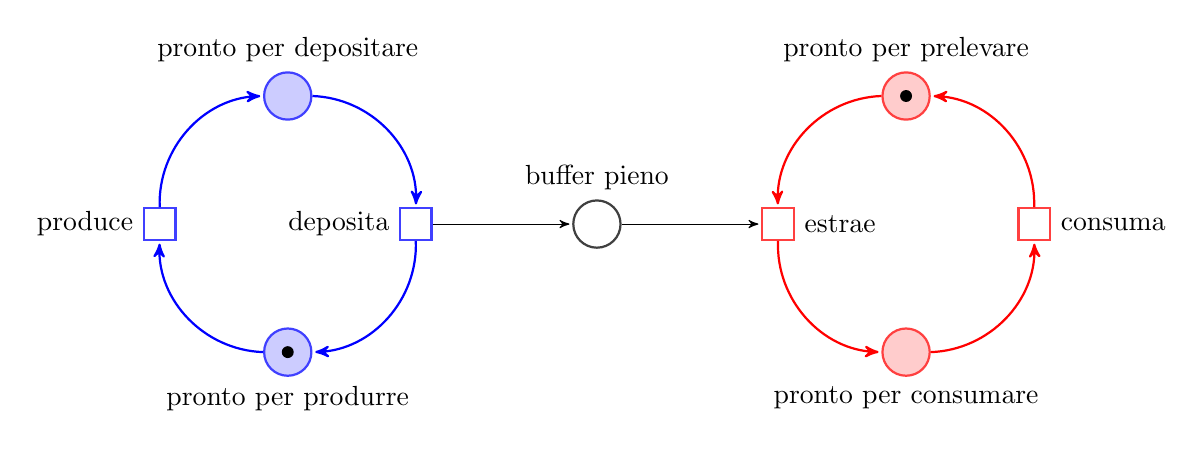
\begin{tikzpicture}[node distance=2.3cm,>=stealth',bend angle=45,auto]
    
      \tikzstyle{place}=[circle,thick,draw=blue!75,fill=blue!20,minimum size=6mm]
      \tikzstyle{transition}=[rectangle,thick,draw=blue!75,minimum size=4mm]
    
        \node [place, tokens=1] (p1)    [label=below:\mbox{pronto per produrre}]         {}; %P1
        \node [transition] (p) [above left of=p1, label=left:\mbox{produce}] {}                   %this is new p
            edge [pre ,bend right, blue,thick]  (p1);
        \node [place] (c1) [above right of=p, label=above:\mbox{pronto per depositare}] {};      %P2
        \node [transition] (p) [above left of=p1] {} %this is new p
            edge [post ,bend left,blue,thick]  (c1);
        \node [transition] (d) [above right of=p1,label=left:\mbox{deposita}] {} %this is d
            edge [pre ,bend right,blue,thick]  (c1)
            edge [post, bend left,blue,thick]  (p1);
            
        \node [place, fill=white,draw=black!75] (b) [right of=d, label=above:\mbox{buffer pieno}] {};
        \node [transition] (d) [above right of=p1] {} %this is d
            edge [post]  (b);
        \node [transition] (e) [right of=b] {} %this is d
            edge [pre]  (b);
        \node[place, tokens=1,fill=red!20,draw=red!75] (c1) [above right of=e, label=above:\mbox{pronto per prelevare}] {};
        \node[place, fill=red!20,draw=red!75] (c2) [below right of=e,label=below:\mbox{pronto per consumare}] {};
        \node [transition,fill=white,draw=red!75] (e) [right of=b,label=right:\mbox{estrae}] {} %this is d
            edge [pre, bend left, red, thick]  (c1)
            edge [post, bend right,red, thick]  (c2);
            
        \node [transition,fill=white,draw=red!75] (c) [above right of=c2,label=right:\mbox{consuma}] {} %this is d
            edge [post, bend right, red, thick]  (c1)
            edge [pre, bend left,red, thick]  (c2);
                
    \end{tikzpicture}
\caption{Buffer pieno}
\label{buffer-pieno}
\end{figure}
\par}

Sia $\Sigma = (B,E,F;c_{in})$ un sistema elementare. Si dice che il sistema è \textbf{senza contatti} sse: \[\forall e\in E,\,\forall c\in C_\Sigma\mbox{ si ha che } ^\bullet e\subseteq c\Rightarrow e^\bullet\cap c=\emptyset\] ovvero per ogni evento e per ogni caso raggiungibile dal caso iniziale succede sempre che se le precondizioni sono vere, ovvero $^\bullet e\subseteq c$, allora le postcondizioni sono false, ovvero disgiunte dal caso considerato ($e^\bullet\cap c=\emptyset$)

Il quesito che ci poniamo è se è possibile trasformare un sistema elementare $\Sigma$, con contatti, in uno $\Sigma'$, senza contatti, senza però modificarne il comportamento.\\ 
La risposta a questo quesito è affermativa e la procedura consiste nell'aggiungere a $\Sigma$ il complemento di ogni condizione che crea situazione di contatto, ottenendo così un sistema $\Sigma'$ con grafo dei casi isomorfo a quello di $\Sigma$.\\ 

Per aggiungere il complemento, data la condizione $x$, si aggiunge la condizione $not\,\, x$ che sarà vera tutte le volte che $x$ è falsa e viceversa. Per ottenere questo risultato la nuova condizione avrà come pre-eventi i post-eventi di $x$ e come post-eventi i pre-eventi di $x$. Ovvero connetto la nuova condizione agli stessi eventi di quella vecchia ma con archi orientati in senso opposto. Ovviamente le inizializzazioni delle due condizioni dovranno essere opposte (una vera e l'altra falsa).

Se un sistema è senza contatti, sia $\Sigma = (B,E,F;c_{in})$ un sistema elementare \textbf{senza contatti}. Sapendo che se le precondizioni di un evento sono vere allora sicuramente le postcondizioni di quell'evento sono false in quel caso. Quindi se un sistema elementare $|Sigma$ è senza contatti allora per verificare che un evento $e$ sia abilitato in un caso raggiungibile $c$ è sufficiente verificare che le precondizioni di $e$ siano vere . In maniera formale quindi si ha che: 
\[c[e\mbox{ sse } ^\bullet e\subseteq c,\,\,\mbox{ con } e\in E,c\in C_\Sigma\] 

Avendo queste informazioni posso andare a utilizzare una formula più semplice, nella la figura \ref{buffer-pieno} vista in precedenza aggiungendo la condizione complemento si ottiene:

{
\begin{figure}[H]
    \centering
    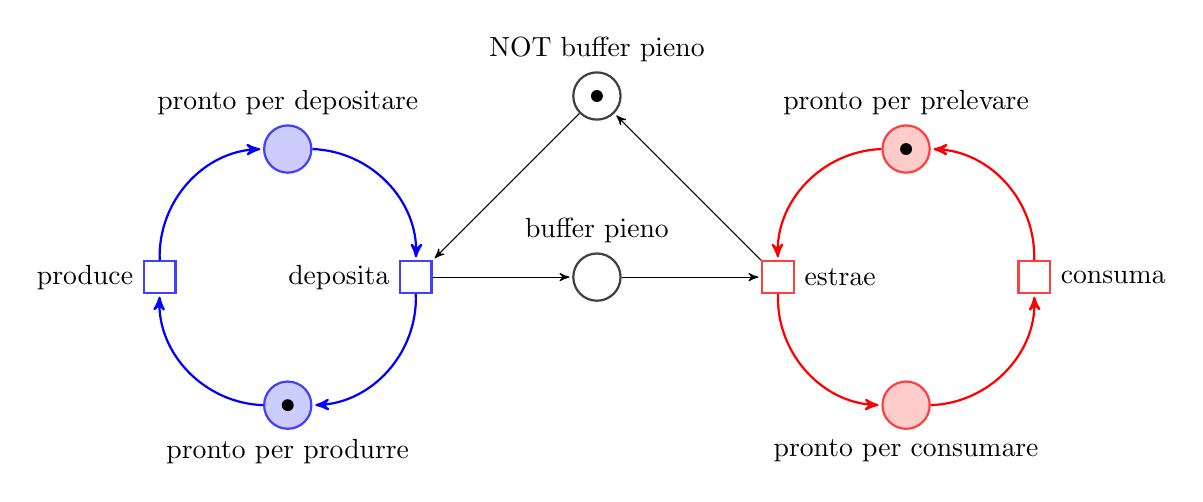
\begin{tikzpicture}[node distance=2.3cm,>=stealth',bend angle=45,auto]
    
      \tikzstyle{place}=[circle,thick,draw=blue!75,fill=blue!20,minimum size=6mm]
      \tikzstyle{transition}=[rectangle,thick,draw=blue!75,minimum size=4mm]
    
        \node [place, tokens=1] (p1)    [label=below:\mbox{pronto per produrre}]         {}; %P1
        \node [transition] (p) [above left of=p1, label=left:\mbox{produce}] {}                   %this is new p
            edge [pre ,bend right, blue,thick]  (p1);
        \node [place] (c1) [above right of=p, label=above:\mbox{pronto per depositare}] {};      %P2
        \node [transition] (p) [above left of=p1] {} %this is new p
            edge [post ,bend left,blue,thick]  (c1);
        \node [transition] (d) [above right of=p1,label=left:\mbox{deposita}] {} %this is d
            edge [pre ,bend right,blue,thick]  (c1)
            edge [post, bend left,blue,thick]  (p1);
            
        \node [place, fill=white,draw=black!75] (b) [right of=d, label=above:\mbox{buffer pieno}] {};
        
        \node [transition] (d) [above right of=p1] {} %this is d
            edge [post]  (b);
        \node [transition] (e) [right of=b] {} %this is d
            edge [pre]  (b);
        \node [place,tokens=1, fill=white,draw=black!75] (notb) [above of=b, label=above:\mbox{NOT buffer pieno}] {}
            edge [pre]  (e)
            edge [post]  (d);
        \node[place, tokens=1,fill=red!20,draw=red!75] (c1) [above right of=e, label=above:\mbox{pronto per prelevare}] {};
        \node[place, fill=red!20,draw=red!75] (c2) [below right of=e,label=below:\mbox{pronto per consumare}] {};
        \node [transition,fill=white,draw=red!75] (e) [right of=b,label=right:\mbox{estrae}] {} %this is d
            edge [pre, bend left, red, thick]  (c1)
            edge [post, bend right,red, thick]  (c2);
            
        \node [transition,fill=white,draw=red!75] (c) [above right of=c2,label=right:\mbox{consuma}] {} %this is d
            edge [post, bend right, red, thick]  (c1)
            edge [pre, bend left,red, thick]  (c2);
                
    \end{tikzpicture}
\caption{Complemento di buffer pieno}
\label{buffer-pieno-complemento}
\end{figure}
\par}

\subsection{Sequenza}
Sia $\Sigma = (B,E,F;c_{in})$ un sistema elementare, con $c\in C_\Sigma$ un caso raggiungibile dal caso iniziale e $e_1,e_2\in E$ due eventi.\\ 
Si ha che $e_1$ ed $e_2$ sono \textbf{in sequenza} nel caso raggiungibile $c$ sse: \[c[e_1>\wedge\, \neg c[e_2\wedge c[e_1e_2>\] ovvero in $c$ è abilitato $e_1$ ma non $e_2$ ma, dopo lo scatto di $e_1$, $e_2$ diventa abilitato. Quindi in $c$ è possibile attivare prima $e_1$ e poi $e_2$ in sequenza.\\ 
Si ha quindi una relazione di \textbf{dipendenza causale tra $e_1$ ed $e_2$}, ovvero qualche postcondizione di $e_1$ è precondizione di $e_2$ (che quindi può occorrere solo se precedentemente è occorso $e_1$).
\section{Lezione del 25 novembre}
\subsection{Situazioni fondamentali}
Nella lezione precedente abbiamo visto la sequenza, definita come un $c[e_1 > \land \neg c[e_2 \land c[e_1e_2$ che mostrava anche il fatto di avere una relazione di \textbf{dipendenza causale} tra $e_1$ ed $e_2$.

\subsubsection{Concorrenza}
Sia $\Sigma = (B,E,F, c_{in})$ un sistema elementare con $c \in C_{\Sigma};\ e_1,e_2 \in E$. Diciamo che i due eventi sono concorrenti in un caso $c$, se e solo se $c[\{e_1e_2\} >$. \\

\begin{center}
    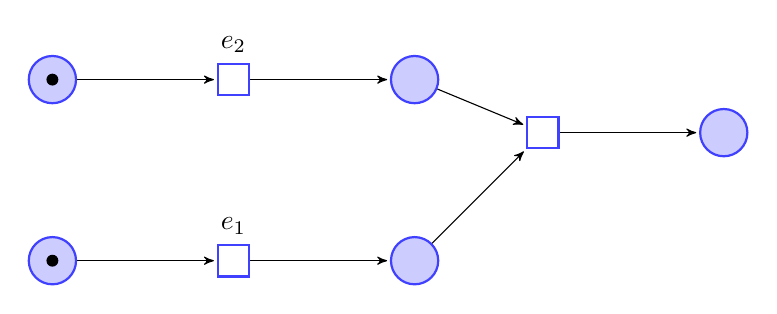
\begin{tikzpicture}[node distance=2.3cm,>=stealth',bend angle=45,auto]
        \tikzstyle{place}=[circle,thick,draw=blue!75,fill=blue!20,minimum size=6mm]
        \tikzstyle{transition}=[rectangle,thick,draw=blue!75,minimum size=4mm]
        
        \node [place, tokens=1] (p1)     {}; %P1
        \node [transition] (p13) [right of=p1, label=above:$e_2$] {}                   %this is new p
            edge [pre]  (p1);
        \node [place] (p3) [right of=p13]   {} %P1
            edge [pre] (p13);
            
        \node [place, tokens=1] (p2) [below of=p1]   {}; %P1
        \node [transition] (p24) [right of=p2, label=above:$e_1$] {}                   %this is new p
            edge [pre]  (p2);
        \node [place] (p4) [right of=p24]   {}
            edge [pre]  (p24);%P1
        \node [transition] (p24p13) [above right of=p4] {}                   %this is new p
            edge [pre]  (p4)
            edge [pre]  (p3);
        \node [place] (p5) [right of = p24p13] {}
            edge [pre]  (p24p13);
    \end{tikzpicture}
\end{center}

Quindi abbiamo due eventi che sono indipendenti, che non hanno quindi pre e post condizioni/ che interferiscono, e che sono abilitati in $c$. E quindi i due eventi possono occorrere in un unico passo.

\subsubsection{Conflitto}
Sia $\Sigma = (B,E,F, c_{in})$ un sistema elementare con $c \in C_{\Sigma};\ e_1,e_2 \in E$. Diciamo che i due eventi sono in conflitto in un caso $c$, se e solo se $c[e_1> \land \ c[e_2> \land \neg c[\{e_1e_2\} > $. \\

In poche parole in questo caso abbiamo che entrambi sono abilitati, come nella concorrenza, ma l'occorrenza di uno disabilita l'altro.


\begin{figure}[H]
\centering
\begin{subfigure}{.5\textwidth}
  \begin{center}
    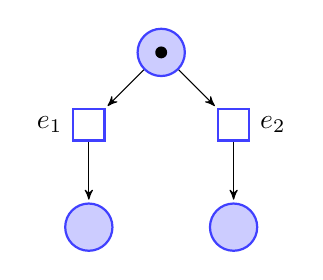
\begin{tikzpicture}[node distance=1.3cm,>=stealth',bend angle=45,auto]
        \tikzstyle{place}=[circle,thick,draw=blue!75,fill=blue!20,minimum size=6mm]
        \tikzstyle{transition}=[rectangle,thick,draw=blue!75,minimum size=4mm]
        
        \node [place, tokens=1] (p1)     {}; %P1
        \node [transition] (p11) [below left of=p1, label=left:$e_1$] {}                   %this is new p
            edge [pre]  (p1);
        \node [transition] (p12) [below right of=p1, label=right:$e_2$] {}                   %this is new p
            edge [pre]  (p1);
            
        \node [place] (p123) [below of=p12]   {} %P1
            edge [pre] (p12);
        \node [place] (p113) [below of=p11]   {} %P1
            edge [pre] (p11);
    \end{tikzpicture}
    \caption{in avanti: forward}
\end{center}
\end{subfigure}%
\begin{subfigure}{.5\textwidth}
\begin{center}
    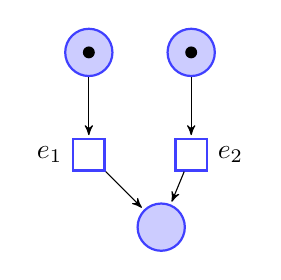
\begin{tikzpicture}[node distance=1.3cm,>=stealth',bend angle=45,auto]
        \tikzstyle{place}=[circle,thick,draw=blue!75,fill=blue!20,minimum size=6mm]
        \tikzstyle{transition}=[rectangle,thick,draw=blue!75,minimum size=4mm]
        
        \node [place, tokens=1] (p1)     {}; %P1
        \node [place, tokens=1] (p2)  [left of=p1]   {}; %P1
        \node [transition] (p11) [below of=p1, label=right:$e_2$] {}                   %this is new p
            edge [pre]  (p1);
        \node [transition] (p12) [below of=p2, label=left:$e_1$] {}                   %this is new p
            edge [pre]  (p2);
        \node [place] (p123) [below right of=p12]   {} %P1
            edge [pre] (p11)
            edge [pre] (p12);
    \end{tikzpicture}
    \caption{all'indietro: backward}
\end{center}
\end{subfigure}%
\end{figure}

In questi tipi di conflitti, modelli, non viene specificato quele dei due eventi scatterà. Sappiamo solamente che se uno dei due scatta, l'altra avrà delle post condizioni vere che non gli permettono di scattare. 

Nel caso in cui prendiamo una possibile configurazione successiva, ad esempio ci ritroviamo:
\begin{figure}[H]
\centering
\begin{subfigure}{.5\textwidth}
  \begin{center}
    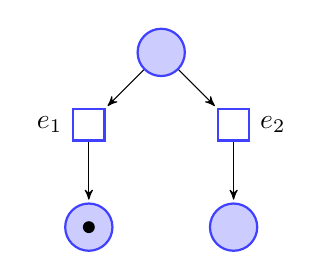
\begin{tikzpicture}[node distance=1.3cm,>=stealth',bend angle=45,auto]
        \tikzstyle{place}=[circle,thick,draw=blue!75,fill=blue!20,minimum size=6mm]
        \tikzstyle{transition}=[rectangle,thick,draw=blue!75,minimum size=4mm]
        
        \node [place] (p1)     {}; %P1
        \node [transition] (p11) [below left of=p1, label=left:$e_1$] {}                   %this is new p
            edge [pre]  (p1);
        \node [transition] (p12) [below right of=p1, label=right:$e_2$] {}                   %this is new p
            edge [pre]  (p1);
            
        \node [place ] (p123) [below of=p12]   {} %P1
            edge [pre] (p12);
        \node [place, tokens=1] (p113) [below of=p11]   {} %P1
            edge [pre] (p11);
    \end{tikzpicture}
    \caption{in avanti: forward}
\end{center}
\end{subfigure}%
\begin{subfigure}{.5\textwidth}
\begin{center}
    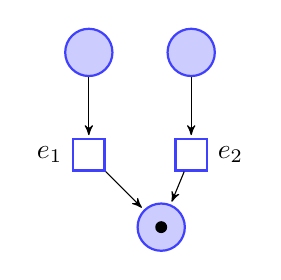
\begin{tikzpicture}[node distance=1.3cm,>=stealth',bend angle=45,auto]
        \tikzstyle{place}=[circle,thick,draw=blue!75,fill=blue!20,minimum size=6mm]
        \tikzstyle{transition}=[rectangle,thick,draw=blue!75,minimum size=4mm]
        
        \node [place] (p1)     {}; %P1
        \node [place] (p2)  [left of=p1]   {}; %P1
        \node [transition] (p11) [below of=p1, label=right:$e_2$] {}                   %this is new p
            edge [pre]  (p1);
        \node [transition] (p12) [below of=p2, label=left:$e_1$] {}                   %this is new p
            edge [pre]  (p2);
        \node [place , tokens=1] (p123 ) [below right of=p12]   {} %P1
            edge [pre] (p11)
            edge [pre] (p12);
    \end{tikzpicture}
    \caption{all'indietro: backward}
\end{center}
\end{subfigure}%
\end{figure}


Ci chiediamo che cosa sia successo al nostro sistema. Ovvero conoscere che cosa ha portato il sistema nella situazione attuale. \\

Nella figura [(a)] sappiamo che è scattato l'evento $e_1$, quindi qualcosa avrà azionato $e_1$ riportando ulteriori informazioni, invece nella figura [(b)] abbiamo che è vera la post condizioni di entrambi gli eventi e quindi possiamo dire che è scattato uno dei due eventi senza precisamente sapere quale. Questo lo riconosciamo perché nella configurazione precedente era vera sola una delle due, quindi era vera o solo la pre di $e_1$ o solo quella di $e_2$. 

\subsubsection{Confusione}
Il conflitto e la concorrenza interferiscono l'una con l'altra generando confusione. Si hanno principalmente due casi di confusione:
\begin{enumerate}
    \item Il primo caso è una confusione \textbf{asimmetrica}. Consideriamo il fatto che possono scattare contemporaneamente due eventi.
    Nel nostro caso abbiamo gli eventi $e_1$ e $e_2$ che possono scattare in maniera concorrente. Lo scatto mi porta nel nuovo caso $b_4$, $b_5$.
    \begin{center}
        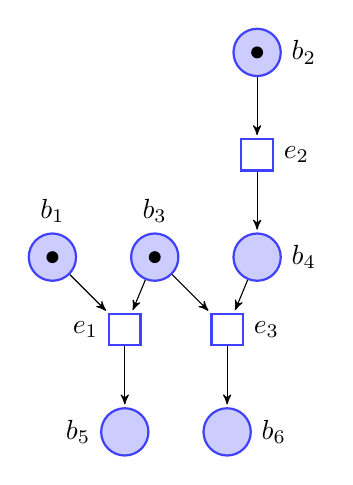
\begin{tikzpicture}[node distance=1.3cm,>=stealth',bend angle=45,auto]
            \tikzstyle{place}=[circle,thick,draw=blue!75,fill=blue!20,minimum size=6mm]
            \tikzstyle{transition}=[rectangle,thick,draw=blue!75,minimum size=4mm]
            
            \node [place, tokens=1] (b2) [label=right:$b_2$]    {}; %P1
            \node [transition] (e2) [below of=b2, label=right:$e_2$] {}                   %this is new p
                edge [pre]  (b2);
            \node [place] (b4) [below of=e2, label=right:$b_4$]    {} %P1
                edge [pre]  (e2);
            \node [place, tokens = 1] (b3) [left of=b4, label=above:$b_3$]    {}; %P1
            \node [place, tokens = 1] (b1) [left of=b3, label=above:$b_1$]    {}; %P1  
            \node [transition] (b1b3) [below right of=b1, label=left:$e_1$] {}                   %this is new p
                edge [pre]  (b1)
                edge [pre]  (b3);
            \node [transition] (b3b4) [below right of=b3, label=right:$e_3$] {}                   %this is new p
                edge [pre]  (b3)
                edge [pre]  (b4);
            \node [place] (p123) [below of=b3b4,label=right:$b_6$]   {} %P1
                edge [pre] (b3b4);
             \node [place] (p123) [below of=b1b3,label=left:$b_5$]   {} %P1
                edge [pre] (b1b3);
        \end{tikzpicture}
    \end{center}
    Se questi vengono eseguiti nello stesso passo, nell'esecuzione di $c[\{e_1e_2\} > c'$ è stato risolto un conflitto? Teniamo conto del fatto che $c = \{b_1,b_2,b_3\} $ e $c = \{b_4,b_5\}$. Non sapendo quale sia stato l'ordine delle due non possiamo stabilire se sia o meno stato risolto un conflitto. \\
    Questo ci porta ad avere due possibilità, entrmabe ammisibili:
    \begin{itemize}
        \item occorre prima $e_1$ senza essere in conflitto 
        \item occorre prima $e_2$ e poi il conflitto tra $e_1$ e $e_3$ viene risolto a favore di $e_1$
    \end{itemize}
    \item Il secondo caso è una confusione \textbf{simmetrica}. Consideriamo il fatto che abbiamo due eventi entrambi abilitati e i due possono occorrere contemporaneamente.
    Nel nostro caso abbiamo gli eventi $e_1$ e $e_3$ che possono occorrere in maniera concorrente. Passando dallo stato $b_1$, $_2$ allo stato $b_3$, $_5$
    \begin{center}
        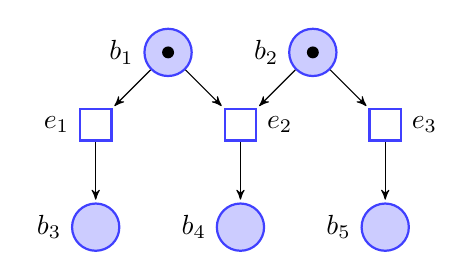
\begin{tikzpicture}[node distance=1.3cm,>=stealth',bend angle=45,auto]
            \tikzstyle{place}=[circle,thick,draw=blue!75,fill=blue!20,minimum size=6mm]
            \tikzstyle{transition}=[rectangle,thick,draw=blue!75,minimum size=4mm]
            
            \node [place, tokens=1] (b2) [label=left:$b_2$]    {}; %P1
            \node [transition] (e2) [below left of=b2, label=right:$e_2$] {}                   %this is new p
                edge [pre]  (b2);
            \node [transition] (e3) [below right of=b2, label=right:$e_3$] {}                   %this is new p
                edge [pre]  (b2);   
            \node [place, tokens=1] (b1) [above left of= e2, label=left:$b_1$]    {} %P1
                edge [post]  (e2);
                
           \node [transition] (e1) [below left of=b1, label=left:$e_1$] {}                   %this is new p
                edge [pre]  (b1);
                
             \node [place] (b3) [below of = e1, label=left:$b_3$]    {} %P1
                edge [pre]  (e1); 
            \node [place] (b4) [below of= e2, label=left:$b_4$]    {} %P1
                edge [pre]  (e2); 
            \node [place] (b5) [below of= e3, label=left:$b_5$]    {} %P1
                edge [pre]  (e3);
        \end{tikzpicture}
    \end{center}
    
    Se scatta $e_1$ il conflitto tra $e_1$ e $e_2$ viene risolto a favore di $e_1$, a questo punto resta solamente $e_3$ abilitato, e quindi scatta.\\
    Se scatta $e_3$ il conflitto tra $e_3$ e $e_2$ viene risolto a favore di $e_3$, a questo punto resta solamente $e_1$ abilitato, e quindi scatta.\\
    Questo comporta che nell'esecuzione di $c[\{e_1e_3\} > c'$ non è possibile stabilire se è stato risolto un conflitto tra $e_1$ ed $e_2$ oppure tra $e_2$ ed $e_3$.\\
    Non è pertanto precisamente specificato chi ha deciso, o chi ha la responsabilità di stabilire chi scatta. 
\end{enumerate} 

\subsection{Sottorete}
Siano $N=(B,E,F)$ e $N_1=(B_1,E_1,F_1)$ due reti elementari. Si dice che $N_1$ è \textbf{sottorete} di $N$  se e solo se: 
\begin{itemize} 
    \item $B_1\subseteq B$, quindi l'insieme delle condizioni della rete $N_1$ è sottoinsieme di quello della rete $N$ 
    \item $E_1\subseteq E$, quindi l'insieme degli eventi della rete $N_1$ è sottoinsieme di quello della rete $N$ 
    \item $F_1=F\cap[(B_1\times E_1)\cup (E_1\times B_1)]$, ovvero la relazione di flusso di $N_1$ è definita come la restrizione della relazione di flusso di $N$ rispetto alle condizioni e $B_1$ e agli eventi $E_1$ (tengo quindi solo gli archi di $N$ che connettono eventi e condizioni di $N_1$) 
\end{itemize}

Esiste inoltre la \textbf{sottorete generata da condizioni}.\\
Si dice che $N_1$ è \textbf{sottorete generata da} $B_1$ di $N$ (ovvero di sottorete generata da un insieme di condizioni)  se e solo se: 
\begin{itemize}
    \item $B_1\subseteq B$, quindi l'insieme delle condizioni della rete $N_1$ è sottoinsieme di quello della rete $N$ 
    \item $E_1=  ^\bullet B_1\cup B_1^\bullet$, ovvero come eventi si hanno tutti quegli eventi che sono collegati in $N$ alle condizioni incluse nell'insieme di condizioni $B_1$, prendendo quindi tutti i pre-eventi e i post-eventi delle condizioni dell'insieme $B_1$ 
    \item $F_1=F\cap[(B_1\times E_1)\cup (E_1\times B_1)]$, ovvero la relazione di flusso di $N_1$ è definita come la restrizione della relazione di flusso di $N$ rispetto alle condizioni $B_1$ e agli eventi $E_1$ 
\end{itemize} 
Non ho quindi una sottorete generata da un insieme arbitrario di condizioni ed eventi ma questi ultimi sono direttamente presi in relazione all'insieme delle condizioni scelto.\\

Esiste inoltre la \textbf{sottorete generata da eventi}.\\
Siano $N=(B,E,F)$ e $N_1=(B_1,E_1,F_1)$ due reti elementari.\\ 
Si dice che $N_1$ è \textbf{sottorete generata da} $E_1$ di $N$ (ovvero di sottorete generata da un insieme di eventi)  se e solo se: 
\begin{itemize} 
    \item $B_1= ^\bullet E_1\cup E_1^\bullet$, ovvero come condizioni si hanno tutte quelle condizioni che sono collegati in $N$ agli eventi inclusi nell'insieme di eventi $E_1$, prendendo quindi tutte e precondizioni e le postcondizioni degli eventi dell'insieme $E_1$ 
    \item $E_1\subseteq E$, quindi l'insieme degli eventi della rete $N_1$ è sottoinsieme di quello della rete $N$ 
    \item $F_1=F\cap[(B_1\times E_1)\cup (E_1\times B_1)]$, ovvero la relazione di flusso di $N_1$ è definita come la restrizione della relazione di flusso di $N$ rispetto alle condizioni $B_1$ e agli eventi $E_1$ 
\end{itemize} 
Non ho quindi una sottorete generata da un insieme arbitrario di condizioni ed eventi ma le prime sono direttamente prese in relazione all'insieme degli eventi scelto

\subsection{Operazioni di Composizione per Reti di Petri}
Data una rete $N=(B,E,F,c_0)$ questa può essere ottenuta componendo altre reti di Petri. Si hanno in letteratura 3 modi principali:
\begin{enumerate}
    \item la \textbf{composizione sincrona}
    \begin{figure}[H]
\centering
\begin{subfigure}{.5\textwidth}
  \begin{center}
   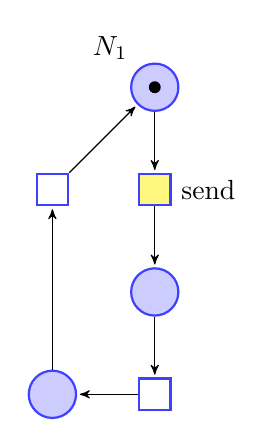
\begin{tikzpicture}[node distance=1.3cm,>=stealth',bend angle=45,auto]
        \tikzstyle{place}=[circle,thick,draw=blue!75,fill=blue!20,minimum size=6mm]
        \tikzstyle{transition}=[rectangle,thick,draw=blue!75,minimum size=4mm]
        
        \node [place, tokens=1] (b2) [label=above left:$N_1$]    {}; %P1
        \node [transition,fill=yellow!50 ] (e2) [below of=b2, label=right:\mbox{send}] {}                   %this is new p
            edge [pre]  (b2);
        \node [place] (b1) [below of= e2]    {} %P1
            edge [pre]  (e2);
        \node [transition] (e1) [below of=b1] {}                   %this is new p
            edge [pre]  (b1);
        \node [place] (b3) [left of = e1]    {} %P1
            edge [pre]  (e1); 
        \node [transition] (b4) [left of= e2]    {} %P1
            edge [pre]  (b3)
            edge [post] (b2); 
    \end{tikzpicture}
\end{center}
\end{subfigure}%
\begin{subfigure}{.5\textwidth}
\begin{center}
     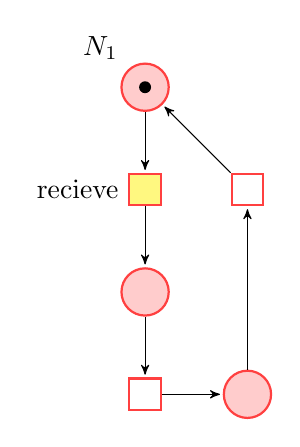
\begin{tikzpicture}[node distance=1.3cm,>=stealth',bend angle=45,auto]
        \tikzstyle{place}=[circle,thick,draw=red!75,fill=red!20,minimum size=6mm]
        \tikzstyle{transition}=[rectangle,thick,draw=red!75,minimum size=4mm]
        
        \node [place, tokens=1] (b2) [label=above left:$N_1$]    {}; %P1
        \node [transition,fill=yellow!50 ] (e2) [below of=b2, label=left:\mbox{recieve}] {}                   %this is new p
            edge [pre]  (b2);
        \node [place] (b1) [below of= e2]    {} %P1
            edge [pre]  (e2);
        \node [transition] (e1) [below of=b1] {}                   %this is new p
            edge [pre]  (b1);
        \node [place] (b3) [right of = e1]    {} %P1
            edge [pre]  (e1); 
        \node [transition] (b4) [right of= e2]    {} %P1
            edge [pre]  (b3)
            edge [post] (b2); 
    \end{tikzpicture}
\end{center}
\end{subfigure}%
\end{figure}
    Portandoci ad ottenere, quando vogliamo unire i due campi, la seguente rete:
    \begin{figure}[H]
        \centering
        \includegraphics[scale=.5]{IMM/sincro.PNG}
    \end{figure}
     Lo scatto dell'evento, in maniera sincrona, rende vere le postcondizioni nelle due componenti e false le due precondizioni.\\
    \item la \textbf{composizione asincrona}
    Supponiamo di avere i modelli di due componenti, $N_1$, che invia in un canale un messaggio (per esempio in un buffer), e $N_2$, che riceverà il messaggio solo quando esso sarà disponibile:
    \begin{figure}[H]
        \centering
        \includegraphics[scale=.5]{IMM/comp_asi.PNG}
    \end{figure}
    In questo caso, a differenza dell'esempio precedente, non identifichiamo eventi ma condizioni. Identifico quindi il canale (le due condizioni) come uno solo, che avrà il pre-evento in una componente e il post-evento nell'altra.\\ 
    Quindi il pre-evento, nella componente $N_1$, può scattare solo se questa nuova condizione condivisa è libera, indipendentemente dalla componente $N_2$. L'evento in $N_2$ può scattare solo se la condizione condivisa è marcata, indipendentemente dallo stato della prima componente, liberando il canale di comunicazione.\\
    \begin{figure}[H]
        \centering
        \includegraphics[scale=.5]{IMM/comp_asi2.PNG}
    \end{figure}
    \item la \textbf{composizione mista, tra sincrona e asincrona}
\end{enumerate}

\subsection{Processi non sequenziali}
Parliamo ora di sistemi non sequenziali, ad ordini parziali.\\ 
Definiamo $N=(B,E,F)$ come una \textbf{rete causale}, detta anche rete di occorrenze senza conflitti, se e solo se:
\begin{itemize}
    \item $\forall b\in B:|^{\bullet}b|\leq 1\land |b^{\bullet}|\leq 1$, ovvero non si hanno conflitti, quindi per ogni condizione si ha al più un pre evento e un post evento (avendo quindi al più un arco entrante e al più uno uscente)
    \item $\forall x,y\in B\cup E:(x,y)\in F^+\implies (y,x)\not\in F^+$, ovvero non si hanno cicli, quindi presi due elementi collegati da una sequenza di archi orientati, avendo un cammino tra i due elementi ($F^+$ è la chiusura transitiva della relazione $F$) non ho anche un cammino opposto tra i due
    \item $\forall e\in E:\{x\in B\cup E| xF^*e\}$ è finito, ovvero si ha un numero finito di pre-elementi di un certo elemento
\end{itemize}

Sono quindi reti che registrano un comportamento e quindi non si hanno conflitti (che in caso sono sciolti registrando solo quello che è effettivamente successo e non quello che potrebbe succedere). Si registra una run del sistema. Non si hanno nemmeno cicli perché ogni ripetizione dell'evento viene concatenata a quella prima (come detto nell'esempio dopo le righe tratteggiate in viola si cominciava da capo).\\ 
 
Ad una rete causale è possibile associare un ordine parziale: $(X,\leq)=(B\cup E, F^*)$. Questo ci dice che un elemento è minore di un altro se esiste un cammino orientato dall'uno all'altro (si specifica che $F^*$ non mi farà mai identificare $x$ con $x$, non ci sarà mai un camino su se stesso).

\subsubsection{Relazioni}
Data una rete causale $N=(B,E,F)$ e dato un ordine parziale $(X, \leq)$ con $X=B\cup E$ si ha che si può interpretare la relazione d'ordine come indipendenza o dipendenza causale.
Siano presi $x,y\in X$ come elementi che occorrono nella storia di $X=B\cup E$ si hanno le seguenti diciture: 
\begin{itemize} 
    \item $x\leq y$ (avendo un cammino da $x$ a $y$) corrisponde a \textbf{$x$ causa $y$}, ovvero si ha una relazione di dipendenza causale tra i due 
    \item $x \mbox{ \textbf{li} }y$ indica che $x\leq y\lor y\leq x$ e quindi corrisponde a \textbf{$x$ e $y$ sono casualmente dipendenti}. Si ha che \textbf{li} può venire letto come \textit{linea} ($x$ in linea con $y$) avendo che uno dei due precede l'altro 
    \item $x \mbox{ \textbf{co} }y$ indica che $\neg(x< y)\land \neg(y < x)$ e quindi corrisponde a \textbf{$x$ e $y$ sono casualmente indipendenti}, avendo che i due elementi non si precedono a vicenda, non sono ordinati. \textbf{co} sta per \textit{concurrency} 
\end{itemize}

\textbf{Line} (li), \textbf{Concurrency} (co) hanno alcune proprietà: sono entrambe simmetriche,\textbf{non} transitive e sono riflessive.

Data una rete causale $N=(B,E,F)$ e dato un ordine parziale $(X, \leq)$ con $X=B\cup E$ definiamo: $C\subseteq X$ come:
\begin{itemize}
    \item \textbf{co-set}  se e solo se $\forall x,y\in C:  x\mbox{ \textbf{co }}y$, quindi $C$ è una clique della relazione \textbf{co}
    \item \textbf{taglio}  se e solo se $C$ è un co-set massimale (tutti gli elementi nel taglio sono in relazione \textbf{co})
\end{itemize}

Definiamo $C$ come co-set massimale  se e solo se $\forall y\in X \land y \notin C$ si ha che: $\exists c\in C: y \mbox{ non è il relazione \textbf{co}  con } c$. Quindi in $C$ definito o come \textbf{co-set} o come \textbf{taglio} si ha che vale la transitività.\\
  
Definiamo: $L\subseteq X$ come:
\begin{itemize}
    \item \textbf{li-set}  se e solo se $\forall x,y\in L:  x\mbox{ \textbf{li }}y$
    \item \textbf{linea}  se e solo se $L$ è un li-set massimale
\end{itemize}

Alcune note:
\begin{itemize}
    \item in un \textbf{co-set} la relazione \textbf{co} è transitiva
    \item in un \textbf{li-set} la relazione \textbf{li} è transitiva.
\end{itemize}
Tagli e linee possono essere fatti sia di condizioni che di eventi.
\section{Lezione del 27 novembre}
Quello che possiamo dire riguardo a una rete causale, è che registra il comportamento di un sistema elementare.\\
All'interno della rete si hanno quindi, con i tagli, possibili ose e solo servazioni di configurazioni possibili nella storia del sistema.\\
Grazie alle reti causali $N=(B,E,F)$, preso un elemento $x\in X$, possiamo definire:
\begin{itemize}
    \item \textbf{past(x)}, ovvero il passato dell'elemento, tutti gli elementi in relazione $\leq$ di $x$
    \item \textbf{future(x)}, ovvero il futuro dell'elemento, tutti gli elementi in relazione $\geq$ di $x$
\end{itemize}
    Visualizzabili, per esempio, nell'immagine, rispettivamente in rosso e blu:
    \begin{figure}[H]
    \centering
    \includegraphics[scale = 0.5]{IMM/cono_di_luce.jpg} 
    \end{figure}
Gli elementi nell'anti-cono (la parte bianca) sono in relazione \textbf{co} con $x$ e quindi possono ese e solo sere concorrenti.

\subsection{k-densità}
Data una rete causale $N=(B,E,F)$ e dato un ordine parziale $(X, \leq)$ con $X=B\cup E$ definiamo che la rete è \textbf{K-densa} se ogni linea ed ogni taglio si intersecano in un punto, tutti hanno un punto comune. Formalmente: \[\forall\,h\in Linee(N),\forall\,c\in Tagli(N):|h\cap c|=1\] Con $Linee(N)$ e $Tagli(N)$ che sono rispettivamente gli insiemi di tutte le linee e dei tagli. Se $N$ è finita è anche \textbf{K-densa}, se sono infinite non è detto.\\

Sia $\Sigma=(S,T,F,c_{in})$ un sistema elementare senza contatti e finito, tale che $S\cup T$ sia finito. Si ha che, con $\phi$ che mappa dalla rete causale al sistema elementare, $\langle N=(B,E,F), \phi\rangle$ è un processo non sequenziale di $\Sigma$ se e solo se:
\begin{itemize}
    \item $(B,E,F)$ è una rete causale dove si ammettono anche condizioni isolate
    \item $\phi:B\cup E \to S\cup T$ è una mappa tale che:
    \begin{itemize}
      \item $\phi(B)\subseteq S, \phi(E)\subseteq T$, far corrispondere alle condizioni, condizioni del sistema, e ad eventi eventi del sistema. 
      \item $\forall x,y\in B\cup E:\phi(x)=\phi(y)\implies (x\leq y)\lor (y\leq x)$, se due elementi della rete corrispondo allo stessa condizione del sistema, questi eventi sono successive occorrenze di quel elemento e quindi nella rete causale sono sicuramente ordinati, non si ha quindi concorrenza
      \item $\forall e\in E:\phi(\,^\bullet e)=\,^\bullet \phi(e)\land\phi(e^\bullet)=\phi(e)^\bullet$ quindi le precondizioni di un evento nella rete causale devono corrispondere alle pre condizioni dell'immagine dell'evento nel sistema elementare (e così anche per le post)
      \item $\phi(Min(N))=c_{in}$, con $Min(N)=\{x\in B\cup E|\nexists y \mbox{tale che }(y,x)\in F\}$, ovvero se vado a prendere gli elementi minimali della rete causali, ovvero tutti quei elementi che non hanno un arco entrante, questi vengono mappati nel caso iniziale del sistema elementare.
    \end{itemize}
\end{itemize}
Se ho queste proprietà la rete causale è una registrazione del sistema elementare.\\ 
In tal caso si ha che $N=(B,E,F)$ è K-densa (sia che sia finita che infinita), avendo il sistema di partenza finito. Le linee sono quindi sottoprocessi sequenziali e i tagli possibili configurazioni sempre raggiungibili.\\ Inoltre si ha che:
\[\forall K \subseteq B, K\mbox{ è B-taglio di } N \mbox{ tale che } K \mbox{ è finito} \land \exists c\in C_\Sigma:\phi(K)=c\] 
Quindi i tagli fatti di condizioni corrispondono a casi raggiungibili. Due punti non possono essere sia in relazione \textbf{co} che in relazione \textbf{li}. Se la retta è dimostrabile essere finita, allora questa è \textbf{k-densa}.\\

Dato un sistema ho tanti processi non sequenziali che rappresentano esecuzioni del sistema. Ci si chiede quindi se ho un unico oggetto che rappresenta tutti i possibili run del sistema.


\section{Lezione del 30 novembre}
Un processo non sequenziale è una rete causale che registra un possibile comportamento e pertanto non presenta né conflitti né cicli.
\subsection{Processo ramificato}
Un processo ramificato altro non è che una rete causale che rappresenta più di un possibile comportamento del sistema. I processi ramificati possono contenere conflitti ma solo in avanti.\\

Una rete elementare $N = (B, E, F)$ è una \textit{rete di occorrenze} $\iff$
\begin{itemize}
    \item $\forall b \in B, |^\bullet b| \leq 1$: solo conflitti in avanti; ogni condizione o rappresenta uno stato iniziale e quindi non ha pre eventi o se ha pre eventi ne ha solo uno.
    \item $\forall x, y \in B \cup E, (x,y) \in F^+ \implies (y,x) \notin F^+$: non ci sono cicli, le ripetizioni di eventi o condizioni vengono registrati come nuovi elementi veri.
    \item $\forall e \in E, \{x \in B \cup E | xF^*e\}$ (il passato di un evento) è finito. 
    \item La relazione di conflitto $\#$ non è riflessiva. Dove la relazione $\# \subseteq X \times X$, con $X = B \cup E$, è definita come segue: 
    \[x \# y \iff \exists e_1, e_2 \in E \; | \; ^\bullet e_1 \cap ^\bullet e_2 \neq \emptyset \; \land \; e_1 \leq x \; \land \; e_2 \leq y\]
    $x$ e $y$ sono in conflitto perché sono in alternativa uno rispetto all’altro perché dipendono rispettivamente da $e_1$ e $e_2$ in conflitto fra loro.
    \end{itemize}
\begin{center}
    Reti causali $\subseteq$ Reti di occorrenze
\end{center}
Per una rete di occorrenze $N$ è possibile assegnare un ordine parziale $(X, \leq) = (B \cup E, F^*)$.\\

Sia $\Sigma = (S,T,F, c_{in})$ un sistema elementare senza contatti e finito, $\langle N = (B,E,F); \phi \rangle$ è un \textit{processo ramificato} di $\Sigma \iff$
\begin{itemize}
    \item $(B,E,F)$ è una rete di occorrenze (si ammettono condizioni isolate)
    \item$\phi : B \cup E \to S \cup T$ è una mappa, che assegna alle condizioni e gli eventi $\to$ le condizione e gli eventi del sistema, tale che:
    \begin{enumerate}
        \item $\phi(B)\subseteq S, \phi(E)\subseteq T$, ovvero che le condizioni vengano mappate nelle condizioni del sistema, e gli eventi negli eventi del sistema. 
        \item $\forall e_1, e_2 \in E: (^\bullet e_1 = {^\bullet e_2} \; \land \; \phi(e_1)= \phi(e_2)) \implies e_1 = e_2$, e quindi se due eventi hanno le stesse precondizioni e corrispondono allo stesso evento del sistema allora necessariamente devono essere lo stesso evento. 
        \item $\forall e \in E, \phi(^\bullet e) = {^\bullet \phi(e)} \; \land \; \phi(e ^\bullet) = {\phi(e)^\bullet}$, in altre parole di ogni evento, le sue precondizioni e postcondizioni devono coincidere con l’immagine delle precondizioni e postcondizioni.
        \item $\phi(\min(N)) = c_{in}$, significa che il taglio iniziale (fatto di condizioni) deve corrispondere alla configurazione (caso) iniziale del sistema.
    \end{enumerate}
\end{itemize}

\subsection{Sottoprocesso e Unfolding}
Prima di poter introdurre l'unfolding, dobbiamo prima dare la definizione di sottoprocesso. \\
Sia $\Sigma = (S,T,F, c_{in})$ un sistema elementare senza contatti e finito e siano $\Pi_1 = \langle N_1; \phi_1 \rangle$, $\Pi_2 = \langle N_2; \phi_2 \rangle$ processi ramificati di $\Sigma$. \\
Allora diciamo che $\Pi_1 = \langle N_1; \phi_1 \rangle$ è un \textit{prefisso} di $\Pi_2 = \langle N_2; \phi_2 \rangle \iff$ $N_1$ è una sottorete di $N_2$ e $\phi_{2|N_1} = \phi_1$ ($\phi_2$ ristretto a $N_1$ è uguale a $\phi_1$). \\

$\Sigma$ ammette un unico processo ramificato che è massimale rispetto alla relazione di prefisso tra processi. Tale processo massimale è l’\textit{unfolding} di $\Sigma$, denotato $Unf(\Sigma)$.\\

Un processo non sequenziale è un processo ramificato $\Pi = \langle N; \phi \rangle$ tale che $N$ sia una rete causale (senza conflitti), e viene detto \textit{corsa (run)}.

\section{Logiche temporali e model-checking}
I metodi di model-checking rendono possibile l'esaminazione dei modelli formali per determinare se soddisfano determinate proprietà di nostro interesse. 
\subsection{Correttezza dei programmi concorrenti}
Dato l'esempio Java, dove viene rappresentato un sistema Consumatore Produttore che interagiscono in modo concorrente, gestito tramite Thread, abbiamo compreso che questo non è un caso sempre possibile, non sempre abbiamo un programma che effettua la gestione per noi. Ci sono però dei metodi che ci vengono incontro per capire come garantire, o capire, la correttezza dei programmi concorrenti.\\
Alcune delle proprietà che devono essere garantite da un programma, affinché possiamo affermare la corretta gestione delle concorrenze, sono:
\begin{itemize}
    \item ogni oggetto prodotto viene prima o poi consumato
    \item nessun oggetto viene consumato più di una volta
    \item il sistema non raggiunge mai uno stato di deadlock
    \item due processi non si trovano mai contemporaneamente nella sezione critica
    \item se un processo richiede l’accesso alla sezione critica, prima o poi avrà il permesso. 
\end{itemize} 
Ci sono sistemi per i quali non è possibile applicare la logica di Hoare: si tratta di sistemi concorrenti. \\
La logica di Hoare si può adattare in una certa misura a sistemi concorrenti ma solo per programmi che obbediscono allo schema generale: dati d’ingresso, elaborazione e stato finale. \\
Per sistemi con un comportamento potenzialmente infinito nel tempo bisogna trovare un altro metodo.

\subsection{Sistemi reattivi}
Sono sistemi concorrenti, distribuiti e asincroni, che non obbediscono al paradigma input-computazione-output e pertanto non è possibile analizzarli con gli strumenti della logica di Hoare.
All’interno di un sistema ci possono essere dei componenti sequenziali con un compito limitato nel tempo la cui correttezza può essere dimostrata utilizzando la logica di Hoare.

\subsection{Analisi di sistemi concorrenti}
Problema: stabilire se un sistema reattivo è corretto.\\
Metodo: si esprime il criterio di correttezza come formula di un opportuno linguaggio logico, si rappresenta (modella) il sistema nella forma di \textit{sistemi di transizioni} e si valuta se la formula è vera nel sistema di transizioni.\\
Strumenti: sistemi di transizioni (modelli di Kripke), logiche temporali e algoritmi.

\subsection{Sistemi di transizioni}
Gli elementi essenziali di un sistema di transizioni son gli \textbf{stati} e \textbf{transizioni di stato}.
\[A = (Q, T)\]
dove $Q$ è l’insieme degli stati e $T \subseteq Q \times Q$ è l’insieme delle transizioni di stato. Deduciamo che un sistema di transizioni è finito se l’insieme degli stati è finito.
In un sistema di transizioni, un cammino è una sequenza di stati in cui ogni coppia di stati adiacenti è legata da una transizione: \[\pi = q_0 q_1 \dots \; | \; \forall i, \; (q_i, q_{i+1}) \in f\]
Un cammino massimale è un cammino che non può essere ulteriormente esteso: 
\begin{itemize}
    \item è finito se termina in uno stato dal quale non esce alcuna transizione
    \item è infinito se percorre infinite volte uno o più stati.
\end{itemize}
Il suffisso di ordine $i$ di $\pi$ è il cammino $\pi^{(i)} = q_i q_{i+1} \dots$.

\subsection{Modello di Kripke}


Sia $Z = \{z_1, z_2, \dots \}$ l’insieme di proposizioni atomiche.
Dato un sistema di transizioni $A = (Q, T)$, si associa a ogni stato $q \in Q$, l’insieme delle proposizioni atomiche che sono vere in quello stato: \[I : Q \to 2^{AP}\]
$2^Z$ perché è l’insieme potenza di $AP$ (l’insieme di tutti i sottoinsiemi di $AP$). 

Un modello di Kripke è un’estensione del sistema di transizioni ed è definito come: $A = (Q, T, I)$.

{\centering
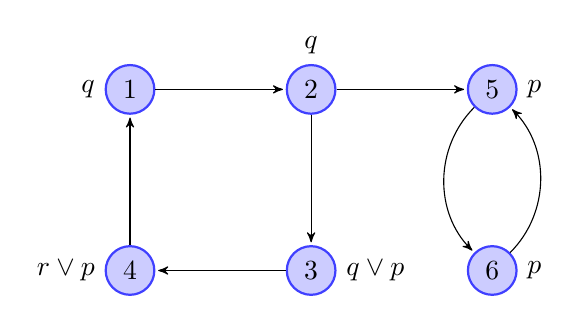
\begin{tikzpicture}[node distance=2.3cm,>=stealth',bend angle=45,auto]
  \tikzstyle{place}=[circle,thick,draw=blue!75,fill=blue!20,minimum size=6mm]
  \tikzstyle{transition}=[rectangle,thick,draw=blue!75,minimum size=4mm]

    \node [place] (uno)   [label=left:$q$] {1}; %P1
    \node [place] (due)   [right of=uno,label=above:$q$] {2}
        edge[pre] (uno); 
    \node [place] (tre)   [below of=due,label=right:$q \lor p$] {3}
        edge[pre] (due); 
    \node [place] (quattro)   [below of=uno,label=left:$r\lor p$] {4}
        edge[pre] (tre)
        edge[post] (uno); 
    \node [place] (cinque)   [right of=due,label=right:$p$] {5}
        edge[pre] (due);
    \node [place] (sei)   [below of=cinque,label=right:$p$] {6}
        edge[post, bend right] (cinque)
        edge[pre, bend left] (cinque);
\end{tikzpicture}
\par}
Supponiamo di avere come preposizioni atomiche $AP = \{p,q,r\}$, abbiamo inoltre $Q=\{1,2,3,4,5,6\}$, e l'insieme delle transizioni $T=\{(1,2),(2,3),(2,5),(5,6) \dots\}$, supponiamo inoltre che la funzione di interpretazione abbia una sua definizione: $I(4) = {p,r}$. Questo viene interpretato come \textit{la funzione I sullo stato quattro, ha come valore vero i valori rappresentati in sua vicinanza, in questo caso $r\lor p$, indica che sono vere entrambe}\\
\subsection{Logica temporale lineare (Linear Temporal Logic, LTL)}
\subsubsection{Sintassi}
\begin{itemize}
    \item $AP = \{p_1, p_2, \dots, p_i, q, r,  \dots\}$	proposizioni atomiche\\
        Non facendo riferimento al tempo, possono essere verificate immediatamente in un certo stato.
    \item $FBF_{LTL}$	insieme delle formule ben formate
        \begin{enumerate}
            \item Ogni proposizione atomica è una formula ben formata.
            \item Le costanti logiche \textbf{true} ($\top$) e \textbf{false} ($\bot$) sono formule ben formate.
            \item Induzione strutturale: se $\alpha$ e $\beta$ sono formule ben formate, anche $\neg \alpha$ e $\alpha \lor \beta$ sono formule ben formate. E quindi lo sono anche $\alpha \land \beta$, $\alpha \implies \beta$ e $\alpha \iff \beta$.
            \item Induzione strutturale (per introdurre le formule temporali): se $\alpha$ e $\beta$ sono formule ben formate lo sono inoltre formule formate anche le seguenti notazioni:
            \begin{enumerate}
                \item $X \alpha$, nel prossimo stato (di computazione)
                \item $F \alpha \;(\lozenge \alpha)$, prima o poi (eventually, finally) $\alpha$ diventerà vera
                \item $G \alpha \; (\square \alpha)$, sempre (globally, always), in questo caso $\alpha$ è sempre vera
                \item $\alpha\  \bigcup \beta$, fino a quando (until), 
            \end{enumerate}
            Per $\alpha \bigcup \beta$ la si potrà ritrovare riscritta $\bigcup(\alpha \cdot \beta)$, questo perché $\alpha \bigcup \beta \equiv \bigcup(\alpha \cdot \beta)$\\
            Alcune volte possiamo ritrovare $\lozenge$ per andare a indicare
        \end{enumerate}
\end{itemize}

\subsubsection{Semantica}
Si interpretano le formule di LTL su un modello di Kripke, procedendo in due fasi:
\begin{enumerate}
    \item Si definisce un criterio per stabilire se una formula $\alpha$ è vera in un cammino massimale $\pi$.
    \item Si dice che la formula è vera rispetto a uno stato $q$ del modello di Kripke se è vera in tutti i cammini massimali che partono da $q$.
\end{enumerate}

\subsubsection{Esempio}
{\centering
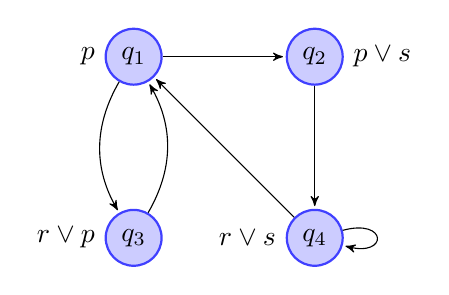
\begin{tikzpicture}[node distance=2.3cm,>=stealth',bend angle=30,auto]
  \tikzstyle{place}=[circle,thick,draw=blue!75,fill=blue!20,minimum size=6mm]
  \tikzstyle{transition}=[rectangle,thick,draw=blue!75,minimum size=4mm]

    \node [place] (uno)   [label=left:$p$] {$q_1$}; %P1
    \node [place] (due)   [right of=uno,label=right:$p \lor s$] {$q_2$}
        edge[pre] (uno); 
    \node [place] (tre)   [below of=due,label=left:$r \lor s$] {$q_4$}
        edge[loop right] (tre)
        edge [pre] (due)
        edge [post] (uno); 
    \node [place] (quattro)   [below of=uno,label=left:$r\lor p$] {$q_3$}
        edge[pre, bend left] (uno)
        edge[post, bend right] (uno); 
\end{tikzpicture}
\par}

Dal che supponiamo di essere interessati a:
\begin{itemize}
    \item $\alpha$ F $s$
    \item $\beta$ F $r$
    \item $\gamma$ G ($p\lor r$)
    \item $\delta$, $p \bigcup s$ 
\end{itemize}

Quello che abbiamo, per quanto riguarda i cammini, dobbiamo vedere se le nostre formule sono vere nei cammini indicati:
\begin{itemize}
    \item $\Pi_1$: $q_1,\ q_3, \ q_1,\ q_3  \ q_1, \ q_3 \dots$ abbiamo che $\quad \Pi_1 \nvDash \alpha,\Pi_1 \vDash \beta,\Pi_1 \vDash \gamma,\Pi_1 \nvDash \delta$
    \item $\Pi_2$: $q_1,\ q_2, \ q_4,\ q_4  \ q_4, \ q_4 \dots$ abbiamo che $\quad \Pi_2 \nvDash \alpha,\Pi_2 \vDash \beta,\Pi_2 \vDash \gamma,\Pi_2 \nvDash \delta$
    \item $\Pi_3$: $q_1,\ q_2, \ q_4,\ q_3, \ q_1, \ q_3 \dots$ abbiamo che $\quad \Pi_3 \vDash \alpha,\Pi_3 \vDash \beta,\Pi_3 \vDash \gamma,\Pi_3 \vDash \delta$
    \item $\Pi_4$: $q_1,\ q_2, \ q_4,\ q_3, \ q_1, \ q_3 \dots$ abbiamo che $\quad \Pi_4 \vDash \alpha,\Pi_4 \vDash \beta,\Pi_4 \vDash \gamma,\Pi_4 \nvDash \delta$
\end{itemize}
\section{Lezione del 9 dicembre}
Dato che noi vogliamo potere determinare la correttezza di una formula delle logiche temporali, dobbiamo andare a considerare tutti i cammini massimali. Per facilitare questo aspetto si possono dividere in famiglie i cammini. Possiamo rappresentare le famiglie con una notazione simile alle espressioni regolari, indichiamo con:
\begin{itemize}
    \item $^*$, indica che si hanno zero o più ripetizioni, ma in numero finito 
    \item $^\omega$, che sta a indicare un numero infinito di ripetizioni 
\end{itemize}
Rispetto alla semantica avevamo detto di avere due fasi da eseguire: la definizione di un criterio per stabilire se una formula $\alpha$ è vera in un cammino massimale $\pi$ e dire che la formula è vera rispetto a uno stato $q$ se è vera in tutti i cammini massimali che partono da $q$.\\

In poche parole, sia $\pi = q_0 q_1 \dots$ un cammino massimale e sia $\alpha$ una formula di LTL. $\pi \vDash \alpha$ significa che $\alpha$ è vera nel cammino $\pi$.\\

Si definisce la relazione $\vDash$ per induzione sulla struttura delle formule.\\

Si supponga che $\alpha$ e $\beta$ siano due formule ben formate e $p$ una proposizione atomica.
\begin{itemize}
    \item $\pi \vDash p \Leftrightarrow p \in I(q_0)$, indica che una proposizione $p$ è vera in un cammino sse $p$ è vera nello stato iniziale del cammino
    \item $\pi \vDash \neg \alpha \Leftrightarrow \pi \nvDash \alpha$, $\neg \alpha$ è vera nel cammino $\pi$ sse $\alpha$ non è vera nel cammino $\pi$
    \item $\pi \vDash \alpha \lor \beta \Leftrightarrow \pi \vDash \alpha \lor \pi \vDash \beta$, diremo invece che $\alpha$, oppure $\beta$, è vera in un cammino, sse una delle due è vera nel cammino $\pi$
\end{itemize}
\subsection{Esempi di formule complesse}
\begin{itemize}
    \item FG$\alpha$, che indica il fatto che $\alpha$ è invariante da un certo istante in poi
    \item GF$\alpha$, con la sola inversione di F e G, otteniamo che $\alpha$ è vera in un numero infinito di stati. Quindi è sempre vero che prima o poi sarà sempre vera $\alpha$
    \item G$\neg(cs_1 \land cs_2)$, dove \textbf{cs} indica \textit{critical section}, che corrisponde alla mutua esclusione. Quindi in nessun stato vale la congiunzione delle 2 proposizioni atomiche.
\end{itemize}
La notazione corrispondente a $req$ rappresenta che c'è una richiesta penedente, mentre con $ack$ denotiamo che è stato spedito un \textit{acknowledgment}
\begin{itemize}
    \item G$(req \implies XF\,ack)$, è sempre vero che se c'è una richiesta pendente, allora prima o poi verrà emesso l'ack a partire dall'istante successivo alla richiesta.
    \item G$(req \implies (req \bigcup ack))$, è sempre vero che se c'è una richiesta, allora sarà valida la richiesta fino a quando verrà emesso l'ack.
    \item G$(req \implies ((req \land \neg ack) \bigcup (ack \land \neg req) )$, è vero che se c'è una richiesta pendente allora si ha che la richiesta vale la richiesta pendente, e non il ack, fino a quando viene emesso l'ack ma diventa falsa req.
\end{itemize}
\subsection{Operatori temporali}
Ipotesi: $\alpha \in FBF$
    \begin{itemize}
    
    \item $\pi \vDash X \alpha \Leftrightarrow \pi^{(1)} \vDash \alpha$, tale formula indica che $\alpha$ dev’essere vera nel cammino che parte dal secondo stato di $\pi$
    \item $\pi \vDash F \alpha \Leftrightarrow \exists i \in \mathbb{N} = \{0,1,2,\dots \} \; | \; \pi^{(i)} \vDash \alpha$, deve esistere un suffisso del cammino, che abbiamo indicato con $\pi^{(i)}$, in cui $\alpha$ sia vera
    \item $\pi \vDash G \alpha \Leftrightarrow \forall i \in \mathbb{N} \; | \; \pi^{(i)} \vDash \alpha$, in questo caso viene indicato che $\alpha$ dev’essere vera in tutti i suffissi di $\pi$ (anche quello iniziale)
    \item $\pi \vDash \alpha U \beta \Leftrightarrow $
        \begin{itemize}
            \item$\exists i \in \mathbb{N} \; | \; \pi^{(i)} \vDash \beta$, ovvero $\pi \vDash F \beta$
            \item$\forall h, \; \, 0 \leq h \leq i, \; \, \pi^{(h)} \vDash \alpha$ 
        \end{itemize}
    S e $i=0$, la seconda clausola non è significativa e pertanto viene considerata vera la formula $\alpha U \beta \Leftrightarrow \pi^{(0)} \vDash \beta$.
\end{itemize}
\subsection{Operatori derivati}
\begin{itemize}
    \item \textbf{Until debole (weak until)}: $\alpha W \beta \equiv G \alpha \lor (\alpha U \beta)$, in tal caso abbiamo che $\beta$ può non diventare mai vera a patto che $\alpha$ rimanga sempre vera
    \item \textbf{Release}: $\alpha R \beta \equiv \beta W (\alpha \land \beta)$, quindi se $\beta$ è sempre vero, oppure a un certo punto diventa  vera anche $\alpha$, e da questo punto in poi $\beta$ può anche diventare falsa.
    \[\pi \vDash \alpha R \beta \Leftrightarrow \forall k \geq 0, \;(\pi^{(k)} \vDash \beta) \lor (\exists h < k \; | \; \pi^{(h)} \vDash \alpha) \]
    Indica che o nel suffisso di ordine $k$ ($\pi^{(k)}$), $\beta$ è vera, oppure in tutti gli stati precedenti è vero $\alpha$
\end{itemize}
\subsection{Formule equivalenti}
\[\alpha \equiv \beta \Leftrightarrow \forall \pi, \; (\pi \vDash \alpha \Leftrightarrow \pi \vDash \beta) \]
Alcuni esempi:
\begin{itemize}
    \item $F \alpha \equiv \alpha \lor XF\alpha$	
    \item $G \alpha \equiv \alpha \land XG\alpha$
    \item $\alpha U \beta \equiv \beta \lor (\alpha \land X (\alpha U \beta))$	o è vera $\beta$ immediatamente o $\alpha$ è vera e dal prossimo stato varrà $\alpha U \beta$
\end{itemize}

\section{Lezione del 11 dicembre}
\begin{itemize}
    \item $FGF \alpha \equiv GF \alpha$	prima o poi sarà sempre vero che prima o poi sarà vera $\alpha$ coincide a è sempre vero che prima o poi sarà vera $\alpha$
    \item $GFG \alpha \equiv FG \alpha$	
\end{itemize}
\subsection{Insiemi minimali di operatori}
\begin{itemize}
    \item $T  \bigcup \alpha$ (true until $\alpha$) $\equiv F \alpha$, occorre che a un certo punto del cammino è vera $\alpha$ e in tutti gli stati precedenti sia vera $T$. MA $T$ è sempre soddisfatta, quindi sostanzialmente si richiede solamente che sia $\alpha$ sia vera. Questo viene mostrato con l'equivalenza. 
    \item $\neg F \neg \alpha$ (non è vero che prima o poi diventa vera $\neg \alpha$) $\equiv G \alpha$, questa equivalenza ci dice che $G$ può essere derivato da $F$ definendolo come la negazione di $F$.
\end{itemize}
Si può dimostrare che l’insieme $\{X, U\}$ forma un insieme minimale di operatori, dal quale si possono derivare tutti gli altri: $F, G, W, R$.

\subsection{Negazioni in LTL}
Quello che ci chiediamo è: cosa significa che non è vero che $F \alpha$? Da non confrontare con la formula  $\neg F \alpha$ \\
Infatti la frase la possiamo riformulare nei termini; \textit{Non è vero che $F \alpha$ equivale a non è vero che in ogni cammino prima o poi $\alpha$ diventa vera e significa che c’è almeno un cammino in cui $\alpha$ è sempre falsa.}\\
Mentre  $\neg F \alpha$  equivale dire che in ogni cammino non è vero che prima o poi $\alpha$ diventa vera, cioè $G \neg \alpha$, in ogni cammino $\alpha$ è sempre falsa. Attenzione $\neg F \alpha$ non è la negazione logica di $F \alpha$.

\subsection{Limiti espressivi di LTL}
LTL non è in grado di esprimere proprietà del tipo “esiste un cammino in cui $\alpha$”.\\
"È possibile" equivale a “Esiste un cammino”.

\subsection{Alberi di computazione}
Sono alberi (grafi aciclici) orientati.
Gli alberi di computazione vengono ricavati da un modello di Kripke partendo da uno stato iniziale che viene utilizzato come radice. Tutti gli archi usciti dallo stato iniziale vengono posti come nodi dell’albero al primo livello e così via.\\
\textit{Computazione}: cammino nell’albero a partire dalla radice.

\subsubsection{Sintassi - Computation Tree Logic}
Proposizioni atomiche: $AP = \{p_1, p_2, \dots, q, r, \dots\}$
Abbiamo delle Formule ben formate,$FBF_{CTL}$, le elenchiamo di seguito: 
\[\forall p \in AP, p \in FBF_{CTL}  \mbox{ e } \forall \alpha, \beta \in FBF_{CTL}\]
\begin{itemize}
    \item $\neg \alpha$, $\alpha \lor \beta \in FBF_{CTL}$
    \item $A X \alpha, E X \alpha \in FBF_{CTL}$	per ogni cammino/esiste un cammino nel quale, nel prossimo stato vale $\alpha$
    \item $A F \alpha, E F \alpha \in FBF_{CTL}$	
    \item $AG \alpha, E G \alpha \in FBF_{CTL}$
    \item $A(\alpha U \beta) \in FBF_{CTL}, E(\alpha U \beta) \in FBF_{CTL}$
\end{itemize}

$A$ (all): quantificatore universale (per ogni cammino)\\
$E$ (exist): quantificatore esistenziale (esiste un cammino tale che)\\

Ogni volta che si usa un operatore temporale bisogna abbinargli un quantificatore. Per esempio: $AFG \alpha$ non è una formula ben formata.\\

A livello sintattico, ci sono formule di LTL che non sono formule di CTL e viceversa. Dal punto di vista semantico, data una formula in CTL è possibile che esista un formula di LTL equivalente.
\section{Confronto tra LTL e CTL}
Molte proprietà interessanti si possono esprimere sia in LTL  sia in CTL:
    \begin{itemize}
    \item Invarianti: nella prima parte abbiamo $AG \neg p$ esprimibile come $G \neg p$
    \item Reattività: in questo caso abbiamo  da una parte $AG(p \to AFq)$ e dall'altra $G(p \to Fq)$

\end{itemize}
Abbiamo poi la Reset property, si esprime nella come \textbf{AG EF}$p$,e sta a indicare che da ogni stato raggiungibile in ogni cammino è sempre possibile raggiungere uno stato nel quale vale $p$. Questa proprietà non la si può esprimere in LTL.\\

Abbiamo la formula $FGp$, in CTL, indica che in ogni cammino prima o poi si raggiungerà uno stato a partire dal quale $p$ rimane sempre vera. Questa proprietà non la si può esprimere in LTL.

{\centering
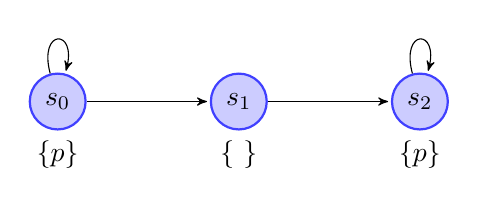
\begin{tikzpicture}[node distance=2.3cm,>=stealth',bend angle=30,auto]
  \tikzstyle{place}=[circle,thick,draw=blue!75,fill=blue!20,minimum size=6mm]
  \tikzstyle{transition}=[rectangle,thick,draw=blue!75,minimum size=4mm]

    \node [place] (uno)   [label=below:$\{p\}$] {$s_0$}
        edge [loop above] (uno); %P1
    
    \node [place] (due)   [right of=uno,label=below:$\{ \ \}$] {$s_1$}
        edge[pre] (uno); 
    \node [place] (tre)   [right of=due,label=below:$\{p\}$] {$s_2$}
        edge [pre] (due)
        edge [loop above] (tre); %P1
\end{tikzpicture}
\par}

Considerato il modello di Kripke sopra, analizziamo la validità di $FG_p$. Andiamo a considerare i cammini massimali
\begin{itemize}
    \item $(s_0)^w$, in questo caso $FG_p$ è verificata
     \item $(s_0 \ s_1) s_2^w$, in questo caso $FG_p$ è verificata
\end{itemize}
Quindi si verifica sempre. Nonostante questo non possiamo trasformala in LTL. Questo perché una possibile traduzione sarebbe AFAG$p$, ma come possiamo notare la \textbf{A} non rispetto la validità della formula. Si trae che:
\[M,s_0 \vDash FGp \quad M,s_0 \nvDash AFAGp\]

Confrontiamo però la formula AFEGp, questo perché comunque io avanzi nell'albero, da qualsiasi punto esiste un cammino in cui $p$ è vera. \textbf{MA} sia:

{\centering
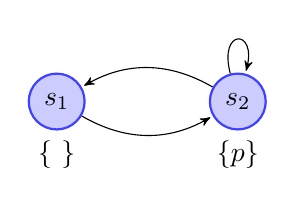
\begin{tikzpicture}[node distance=2.3cm,>=stealth',bend angle=30,auto]
  \tikzstyle{place}=[circle,thick,draw=blue!75,fill=blue!20,minimum size=6mm]
  \tikzstyle{transition}=[rectangle,thick,draw=blue!75,minimum size=4mm]

    \node [place] (uno)   [label=below:$\{ \ \}$] {$s_1$};
    \node [place] (tre)   [right of=uno,label=below:$\{p\}$] {$s_2$}
        edge [pre, bend left] (uno)
        edge [post, bend right] (uno)
        edge [loop above] (tre); %P1
\end{tikzpicture}
\par}
Ci ritroviamo comunque a dire che
\[M,s_1 \nvDash FGp \quad M,s_1 \vDash AFEGp\]

Perché abbiamo un cammino che non rende mai vera $Gp$, è vera però AFAGp. Infatti prima o poi ci sarà un cammino in cui vale \textit{p}.
\subsection{CTL$^*$}
Esiste una logica CTL*, questa estende sia LTL sia CTL, mantenendo i due quantificatori sui cammini, ma eliminando il vincolo di CTL.\\
\textbf{Esempio}: AFG$p \lor$ AFEG $q$ espressa EFG$q$\\

In linea di massima, estendere la capacità espressiva di una logica si paga con un maggior costo computazionale degli algoritmi di model-checking per le formule di quella logica.

\subsection{Equivalenza di modelli rispetto a una logica}
Due modelli di Kripke, $M_1$ e $M_2$, con stati iniziali $q_0$ e $s_0$ si dicono \textit{equivalenti} rispetto a una logica \textbf{L} se, per ogni formula $\alpha \in FBF_L$: \[M_1, q_o \vDash \alpha \iff M_2, s_0 \vDash \alpha\]

\subsection{Insiemi parzialmente ordinati}
Relazione d’ordine parziale su $A$: $\leq$ $\subseteq$ $A \times A$
\begin{enumerate}
    \item \textbf{riflessiva}: $x \leq x$, $\forall x \in A$
    \item \textbf{antisimmetrica}: $(x \leq y \land y \leq x) \implies x = y$, $\forall x, y \in A$
    \item \textbf{transitiva}: $(x \leq y \land y \leq z) \implies x \leq z$, $\forall x,y,z \in A$
\end{enumerate}

Sia $(A, \leq)$ un insieme parzialmente ordinato e $B \subseteq A$. Allora diciamo che $x \in A$ è un \textbf{maggiorante} di $B$ se $y \leq x$, $\forall y \in B$. Mentre $x \in A$ è un \textbf{minorante} di $B$ se $x \leq y$, $\forall y \in B$.\\

Si indica con $B^*$ l’insieme dei maggioranti di $B$ e con $B_*$ l’insieme dei minoranti di $B$.\\
$B$ si dice:
\begin{enumerate}
    \item limitato \textbf{superiormente} se $B^* \neq \emptyset$. 
    \item limitato \textbf{inferiormente} se $B_* \neq \emptyset$.
\end{enumerate}

Per quanto riguarda \textbf{$x \in B$}, questo:
\begin{itemize}
    \item è il \textbf{minimo} di $B$ se $x \leq y$, $\forall y \in B$.
    \item è il \textbf{massimo} di $B$ se $y \leq x$, $\forall y \in B$.
    \item è \textbf{minimale} in $B$ se $y \leq x \implies y = x$.
    \item è \textbf{massimale} in $B$ se $x \leq y \implies y = x$.
\end{itemize}
 
Se $x$ è il minimo di $B^*$, si dice che $x$ è l’estremo superiore (join) di $B$ e si scrive $x = \sup B$ o $x = \bigvee B$. Se $x$ è il massimo di $B_*$, si dice che $x$ è l’estremo inferiore (meet) di $B$ e si scrive $x = \inf B$ o $x = \bigwedge B$. In particolare, se $B = \{x,y\}$, si scrive $x \bigvee y$ per indicare $\bigvee B$ se esiste e $x \bigwedge y$ per $\bigwedge B$ se esiste.\\

Si consideri la logica proposizionale.\\

La nozione di implicazione ha due aspetti: operazione che date due formule costruisce una nuova formula e relazione binaria tra formule.\\
L’implicazione è riflessiva perché qualunque formula $\alpha$ implica se stessa ed è transitiva perché se una formula $\alpha$ implica $\beta$ e la formula $\beta$ implica $\gamma$ allora anche $\alpha$ implicherà $\gamma$.\\

Per quanto riguarda l’antisimmetria, date due formule diverse $\alpha$ e $\beta$ è possibile che $\alpha$ implichi $\beta$ e viceversa. (Esempio: $\alpha \lor \beta \implies \beta \lor \alpha$ e viceversa)\\

Quindi l’implicazione non è una relazione di ordine parziale sull’insieme di tutte le formule bene formate. Si tratta di una relazione di *preordine*, in quanto è riflessiva e transitiva.\\

È possibile trasformare qualunque relazione di preordine in una relazione di ordine parziale su un insieme derivato.
Definita una relazione di equivalenza tra formule, si possono costruire le classi di equivalenza, ovvero insiemi di formule tali che in ogni insieme ci sono formule due a due equivalenti.\\

Con $[FBF_{LP}]_{\equiv}$ si indica l’insieme di tutte le classi di equivalenza, sul quale si può definire una relazione $\implies$ definita nel seguente modo: una certa classe di equivalenza implica un’altra classe di equivalenza se una qualunque delle formule della prima classe implica una qualunque delle formule della seconda classe.\\
$([FBF_{LP}]_{\equiv}, \implies)$ è una relazione di ordine parziale.

\subsection{Reticolo}
Un \textit{reticolo} è un insieme parzialmente ordinato $(L, \leq)$, tale che $\forall x, y \in L$, esistono $x \bigvee y$ (join) e $x \bigwedge y$ (meet).
Un reticolo si dice completo se $\bigvee B$ e $\bigwedge B$ esistono $\forall B \subseteq L$.
\section{Lezione del 16 dicembre}
Partiamo parlando di insiemi parzialmente ordinati e Funzione monotòne. Siano $(A, \leq)$ e $(B, \leq)$ due insiemi parzialmente ordinati.\\ 
Una funzione $f : A \to B$ si dice \textit{monotòna} se, \[\forall x, y \in A \mbox{ vale }x \leq y \implies f(x) \leq f(y)\]
Una funzione è monotòna se preserva la relazione d’ordine.

\subsection{Punti fissi}
Si considera una funzione $f : X \to X$. Un elemento $x \in X$ è un punto fisso di $f$ se $f(x) = x$.
Ci sono i seguenti esempi:
\begin{itemize}
    \item $f: \mathbb{R} \to  \mathbb{R}, \ f(x) = x^2$, l'insieme dei punti fissi sono i punti $\{0,1\}$\\
    La funzione non è monotona, infatti se prendessimo $x= -5$ e $y=-4$, essendo $-5 \leq -4$, non implica che $f(x) \leq f(y)$. Infatti $25 \nleq 16$
    \item $g: \mathbb{R}^+ \to  \mathbb{R}, \ g(x) = log(x)$, l'insieme dei punti fissi sono i punti $\emptyset$\\
    Questa è monotona
    \item $h: \mathbb{R} \to  \mathbb{R}, \ h(x) = x$, l'insieme dei punti fissi sono i punti $\mathbb{R}$\\
    
\end{itemize}

Se $(A, \leq)$ è un insieme parzialmente ordinato e $f:A \to A$ è una funzione monotòna, ci si può chiedere se esistono un minimo e un massimo punto fisso.\\

\subsubsection{Esempio}
Consideriamo $A=2^\mathbb{N}$ e $S \subseteq \mathbb{N}$
Consideriamo le varie funzioni:
\begin{enumerate}
    \item $f(S) = S \cup \{2,7\}$. Tutti i sottoinsiemi che contengono $2$ e $7$ sono punti fissi. La funzione $f(S)$ è monotona, inoltre $\{2,7\}$ rappresenta il punto fisso minimo, mentre $\mathbb{N}$ risulta essere il punto fisso massimo.
    \item $f(S) = S \cap \{2,7,8\}$, in questo esempio la funzione $f(S)$ è monotona, $\{2,7,8\}$ rappresenta il punto fisso massimo, mentre $\emptyset$ risulta essere il punto fisso minimo.
    \item Il terzo esempio diferisce:
    
    {\centering
        \begin{tikzpicture}[node distance=2.3cm,>=stealth',bend angle=30,auto]
        \tikzstyle{place}=[circle,thick,draw=blue!75,fill=blue!20,minimum size=6mm]
        \tikzstyle{transition}=[rectangle,thick,draw=blue!75,minimum size=4mm]
        
            \node [place] (uno)   [] {$1$};
            \node [place] (tre)   [below right of=uno] {$3$}
                edge [pre] (uno);
            \node [place] (due)   [below left of=uno] {$2$}
                edge [pre] (uno);
            
                
            \node [place] (due-4)   [below left of=due] {$4$}
                edge [pre] (due);
            \node [place] (due-5)   [right = 1.95cm of due-4] {$5$}
                edge [pre] (due); 
                
             \node [place] (due-9)   [below right of=due-5] {$9$}
                edge [pre] (due-5);
             \node [place] (due-8)   [below left of=due-5] {$8$}
                edge [pre] (due-5);
            \node [place] (tre-7)   [below right of= tre] {$7$}
                edge [pre] (tre);
            \node [place] (tre-6)   [right= .5cm of due-5] {$6$}
                edge [pre] (tre);
            \node [place] (tre-10)   [below right of = tre-6] {$10$}
                edge [pre] (tre-6);
            \node [place] (tre-11)   [below right of = tre-7] {$11$}
                edge [pre] (tre-7);
            \end{tikzpicture}
    \par}
    Da questo derivano $A = \{1,2 \dots, 11\}$, e ($\mathbb{P}(A), \subseteq$), ovvero insieme delle parti di $A$ ordinata sul contenimento $\subseteq$\\
    La funzione è definita $f:\mathbb{P}(A) \to \mathbb{P}(A)$, dove $f(S) = S \cup \{x \in A | x \mbox{ è il figlio di un } y\in S\}$. Guardiamo alcuni valori di S:
    \begin{itemize}
        \item $f(\{2,6\}) = \{2,6,4,5,10\} \qquad f(\{2,6\}) \neq \{2,6\}$
        \item $f(\{2,6,4,5,10\}) = \{2,6,4,5,10,8,9\} = M $ 
        \item $f(M) = M$ 
        \item $f(\emptyset) = \emptyset$ 
    \end{itemize}
    Il massimo punto fisso è $A$, se non ci fosse $\emptyset$ non ci sarebbe un punto fisso minimo (perché questo non sarebbe unico), ma ci sarebbero i punti fissi minimali rappresentati dalle foglie dell'albero.
\end{enumerate}

\subsection{Teorema di Knaster-Tarski}
Siano $(L, \leq)$ un reticolo completo e $f:L \to L$ una funzione monotòna. Allora $f$ ha un minimo e un massimo punto fisso.
\subsubsection{Dimostrazione per un caso particolare}
$L=2^A$, per un insieme $A$ e sia $f : 2^A \to 2^A$, capire se tale funzione è monotona. \\
Il primo passo consiste nel costruire l’insieme $Z = \{T \subseteq A \; | \; f(T) \subseteq T\}$, dove gli elementi di $Z$ vengono chiamati \textit{punti pre-fissi}. \\ 

L’insieme $Z$ non può essere vuoto, perché tra i sottoinsiemi di $A$ c’è l’insieme $A$ e l’immagine di $A$ dev’essere un sottoinsieme di $A$ e necessariamente sarà contenuta in $A$.\\

Si supponga che $f$ abbia qualche punto fisso, allora per questi punti fissi $p$ vale che $f(p)=p$, quindi se $f$ ha dei punti fissi, $Z$ li contiene tutti.
Si ponga $m = \bigcap Z$.
\[\forall S \in Z \,, m \subseteq S \mbox{ quindi }f(m) \subseteq f(S) \subseteq S\]
Allora sappiamo che $f(m) \subseteq \bigcap Z = m$ che ci porta a concludere che $m \in Z$. Per tanto osserviamo che $m = \min Z$, quindi:
\[f(m) \subseteq m\]
La funzione $f$ è inoltre monotòna, e questo quindi ci porta a concludere che $f(f(m)) \subseteq f(m)$. Ma allora $f(m) \in Z$, e quindi $m \subseteq f(m)$. E come analizzato prima, anche ora possiamo dire che $m$ è il minimo punto fisso di $f$.

\subsection{Funzione continua}
Sia $f : 2^A \to 2^A$ una funzione monotòna. Prese una catena di sottoinsiemi di $A$, ovvero elementi di $2^A$, tale che 
\[X_1 \subseteq X_2 \subseteq \dots \subseteq X_i \subseteq \dots\]  
e la catena delle loro immagini \[f(X_1) \subseteq f(X_2) \subseteq \dots \subseteq f(X_i) \subseteq \dots\] 
Si costruisce (sapendo che $2^A$ è un reticolo completo) l’unione di tutti gli $X_i$ che è un sottoinsieme di $A$.\\
La funzione $f$ si dice \textit{continua} se $f(\bigcup X_i) = \bigcup f(X_i)$.

Normalmente ciò non vale per tutte le funzioni monotòne, ma appunto solo per quelle continue.

\subsection{Teorema di Kleene}
Se $f$ è continua, allora il minimo punto fisso si $f$ si può ottenere calcolando \[f(\O), f(f(\O)), f(f(f(\O))), \dots\] 
e il massimo punto fisso di $f$ si può ottener calcolando \[f(A), f(f(A)), f(f(f(A))), \dots\] (fermandosi quando si arriva a un risultato uguale al precedente).
\subsubsection{Esempi}
Consideriamo $A=2^\mathbb{N}$ e $S \subseteq \mathbb{N}$
Consideriamo le varie funzioni applicate alla funzione di Kleene:
\begin{enumerate}
    \item $f(S) = S \cup \{2,7\}$. Quello che facciamo $f(\emptyset) = \emptyset \cup \{2,7\}$, ma non è il risultato che ci serve, applichiamo ancora la $f(f(\emptyset)) = f(\{2,7\}) = \{2,7\}$, questo infatti rappresenta il punto fisso minimo, mentre $f(\mathbb{N})$ restituisce subito $\mathbb{N}$ e questo risulta essere il punto fisso massimo. 
    \item $f(S) = S \cap \{2,7,8\}$, in questo esempio la funzione $f(\emptyset) = \emptyset$ al primo passaggio e risulta essere il punto fisso minimo. Mentre per il punto massimo troviamo $f(\mathbb{N}) = \mathbb{N} \cap \{2,7,8\}$, quindi $f(f(\mathbb{N})) = f(\mathbb{N} \cap \{2,7,8\}) = \{2,7,8\}$
\end{enumerate}
\section{Algoritmi per LTL}
Automi finiti che riconoscono parole infinite su un alfabeto finito $\Sigma$, detti\textit{ automi di Büchi}, questi vengono rappresentati come $B = (Q, q_0, \delta, F)$, dove:
\begin{itemize}
    \item $Q$: insieme finito di stati (\textit{locations})
    \item $q_0 \in Q$: stato iniziale
    \item $\delta \subseteq Q \times \Sigma \times Q$: relazione di transizione, indica le possibili transizioni di questo automa. Composto da stato di partenza, etichetta e lo stato di arrivo. 
    \item $F \subseteq Q$: insieme degli stati accettanti
\end{itemize}

Una parola infinita $w = a_0 a_1 \dots$ è accettata da $B$ se la sequenza corrispondente di stati $q_0q_1\dots$ passa infinite volte per almeno uno stato in $F$.\\

Si cerca da $q_0$ una transizione uscente etichettata con il simbolo $a_0$, se non esiste ci si ferma e si dice che la parola non è accettata. In caso contrario invece, si passa al nuovo stato e si controlla se esiste un arco uscente etichettato con il secondo simbolo della parola e così via.\\

Il problema $L(B) = \emptyset$ è decidibile.
\subsection{Esempio}
\begin{enumerate}
    \item Osserviamo il seguente automa finito:
        \begin{center}
            \begin{tikzpicture}[shorten >=1pt,node distance=2cm,on grid,auto] 
               \node[state,accepting] (q_0) [] {$q_0$}; 
               \node[state] (q_1) [right=of q_0] {$q_1$}; 
                \path[->] 
                (q_0) edge [bend left] node  {$a$} (q_1)
                      edge [loop left] node {$b$} ()
                (q_1) edge [bend left] node  {$b$} (q_0)
                      edge [loop right] node {$a$} ();
            \end{tikzpicture}
        \end{center}
        
        Siano poi alcune parole infinite, e diciamo se sono accettate o meno dall'automa raffigurato:
        \begin{itemize}
            \item $w_1 = bbbbbbbbb\dots$, questa parola è accettata, rimane in $q_0$ che è accettante. Appartiene quindi al linguaggio dell'automa
            \item $w_2 = bbaaabbbb\dots$, anche questa parola è accettata, infatti dopo 6 mosse rimane sempre in $q_0$.
            \item $w_3 = babababab\dots$, anche questa parola è accettata, si rimane infinite volte nel ciclo $q_o \to q_1$, per tanto passa infinite volte in $q_0$ essendo di conseguenza accettata.
            \item $w_4 = baabbbaaa\dots$, dato che resta un numero finito di volte in $q_1$, e solamente un numero finito di volte in $q_0$, questa parola non è accettata e non fa parte del linguaggio dell'automa. 
        \end{itemize}
    \item Osserviamo un secondo automa finito:
        \begin{center}
            \begin{tikzpicture}[shorten >=1pt,node distance=2cm,on grid,auto] 
               \node[state] (q_0) [] {$q_0$}; 
               \node[state,accepting] (q_1) [right=of q_0] {$q_1$}; 
                \path[->] 
                (q_0) edge [bend left] node  {$\{p\}$} (q_1)
                      edge [loop left] node {$\emptyset$} ()
                (q_1) edge [bend left] node  {$\emptyset$} (q_0)
                      edge [loop right] node {$\{p\}$} ();
            \end{tikzpicture}
        \end{center}
        
    Sottoinsiemi di proposizioni atomiche: $\emptyset$ e $\{p\}$
    \begin{itemize}
        \item $w_1 = \emptyset\{p\}\{p\}\emptyset\{p\}\emptyset\emptyset \dots$, questa non viene accettata
        \item $w_2 = \emptyset\{p\}\emptyset\{p\}\emptyset \dots$, questa invece viene accettata
    \end{itemize}
    Sia GF$\{p\}$ la formula LTL corrispondente all'automa, allora per la formula GF$\{p\}$ diciamo che $p$ è vera in numero infinito di stati in un certo cammino
\end{enumerate}
\subsection{Algoritmo per LTL - Problema}

Il problema sta nel verificare se $\alpha$ è vera in $(M, q_0)$.
\begin{enumerate}
    \item Si costruisce l’automa $B_{\neg \alpha}$, ovvero l’automa che riconosce tutte le parole in cui $\alpha$ non è verificata.
    \item Si trasforma il modello di Kripke $M$ in un automa etichettato da insiemi di proposizioni atomiche.
    \item Si calcola il prodotto sincrono dei due automi $PS$.\\
   \textit{Prodotto sincrono}: automa dato dall’esecuzione in parallelo due automi in modo che procedano con le stesse azioni (etichette). I suoi stati pertanto sono formati dal prodotto cartesiano degli stati dei due automi componenti.\\
   Nel caso in cui, nella coppia di stati correnti, uno degli automi non ha la transizione uscente con l’etichetta considerata, il prodotto sincrono non può avanzare quindi non c’è una transazione nel prodotto sincrono corrispondente a quell’azione.\\
   
   Le parole riconosciute dal prodotto sincrono sono tutte e sole le parole riconosciute da entrambi i due automi.
   \item Se $L(PS) = \emptyset$, allora $M, q_0 \models \alpha$, non c’è nessun cammino nel quale non è verificata la formula $\alpha$.
\end{enumerate}

\subsubsection{Estensione per formule in LTL}
Siano $M = (Q, T, I)$ un modello di Kripke e $\alpha$ una formula.
Si definisce \textit{estensione} di $\alpha$ l’insieme degli stati in cui $\alpha$ è valida, ovvero $[[\alpha]] = \{q \in Q \; | \; M, q \models \alpha\}$.
Si hanno poi alcuni \textit{casi particolari};
\begin{itemize}
    \item $[[T]] = Q$
    \item $[[F]]=\emptyset$
    \item $[[p]] = $ insieme degli stati in cui è vera $p$, con $p \in AP$
\end{itemize}

\subsubsection{Estensione per formule in CTL}
Sia $M = (Q, T, I)$ un modello di Kripke.
\begin{itemize}
    \item Si considera la formula $\alpha \equiv AF\beta$ a cui si associa una funzione $f_{\alpha}: 2^Q \to 2^Q$ tale che 
    \[\forall H \subseteq Q \, ,f_{\alpha}(H) = [[\beta]] \cup \{q \in Q \; | \; \forall (q, q') \in T, \; q' \in H\}\]
    Osservazione: $f_{\alpha}(\emptyset) = [[\beta]]$. Inoltre possiamo dimostrare che $[[\alpha]]$ è il minimo punto fisso di $f_\alpha$.
  \item Si considera la formula $\alpha \equiv EG\beta$ a cui si associa una funzione $g_{\alpha}: 2^Q \to 2^Q$ tale che 
  \[\forall H \subseteq Q \, ,g_{\alpha}(H) = [[\beta]] \cap \{q \in Q \; | \; \forall (q, q') \in T, \; q' \in H\}\]
  Osservazione: $g_{\alpha}(Q) = [[\beta]]$. Inoltre $[[\alpha]]$ è il massimo punto fisso di $g_\alpha$.
\end{itemize}

\subsection{Calcolo $\mu$}
È un linguaggio logico che permette di definire formule ricorsive. \\
Si supponga di avere un solo operatore temporale: $X$. È possibile esprimere la proprietà $EF \alpha$?
\[EF \alpha \equiv \alpha \lor EX\alpha \lor EXEX \alpha \lor \dots\]

Si tratta di una formula infinita ma con una struttura ben definita.
Si raccoglie $EX$ e otteniamo in seguito 
\begin{equation*}
    \begin{split}
        EF \alpha   &\equiv \alpha \lor EX(\alpha \lor EX \alpha \lor EXEX \alpha \lor \dots)\\
                    & \equiv \alpha \lor EX(EF \alpha)
    \end{split}
\end{equation*}
Quest’espressione ha un carattere ricorsivo e verrà scritta in forma compatta come $\mu Y.(\alpha \lor EXY)$\\

Si può fare un ragionamento analogo per $AG \alpha$:
\[AG \alpha \equiv \alpha \land AX\alpha \land AXAX \alpha \land \dots\]
Si tratta di una formula infinita ma con una struttura ben definita. Anche qui si raccoglie $AX$ ottenendo poi:
\begin{equation*}
    \begin{split}
        AG \alpha   & \equiv \alpha \land AX(\alpha \land AX \alpha \land AXAX \alpha \land \dots) \\
                    & \equiv \alpha \land AX(AG \alpha)
    \end{split}
\end{equation*}
Quest’espressione ha un carattere ricorsivo e verrà scritta in forma compatta come $\nu Y.(\alpha \lor AXY)$

Il senso di questo operazione, è quello di poter generalizzare l'idea di definire formule di un linguaggio logico come nelle forme compatte viste sopra, fino ad avere un linguaggio completo che consideriamo come una nuova logica. 
\subsubsection{Sintassi del calcolo $\mu$}
Sia $AP = \{p_1, p_2, \dots, q, r, \dots\}$ l’insieme delle proposizioni atomiche. E siano $\alpha$ e $\beta$ due formule.
\begin{enumerate}
    \item $\alpha \lor \beta$ e $\neg \alpha$ sono formule.
    \item $EX \alpha, AX \alpha$ sono formule.
    \item $\mu Y.f(Y)$ è una formula, dove $f$ è una formula nella quale compare $Y$ (con restrizioni sulle negazioni).
    \item $\nu Y. f(Y)$ è una formula, dove $f$ è una formula nella quale compare $Y$ (con restrizioni sulle negazioni).
\end{enumerate}

La semantica del calcolo $\mu$ è definita su modelli di Kripke attraverso operatori di punto fisso.\\

CTL$^* \subset \mu$-calculus (tutte le proprietà esprimibili in CTL$^*$ sono esprimibili anche in calcolo $\mu$). Il calcolo $\mu$ ha la massima potenza espressiva, un’alta complessità e una potenziale oscurità delle formule.

\subsubsection{Complessità e aspetti algoritmici}
Siano $M$ un modello di Kripke (e $|M|$ la sua dimensione, ovvero il numero di stati) e $f$ una formula (e $|f|$ la sua dimensione).\\
Complessità temporale di CTL: $\mathcal{O}(|M| \times |f|)$\\
Complessità temporale di LTL: $\mathcal{O}(|M| \times 2^{|f|})$\\
Le stime di complessità vanno interpretate perché CTL, anche sembra meno complesso, spesso comporta formule di dimensioni maggiori.\\

Strategie algoritmiche: rappresentazioni simboliche (OBDD), partial order reduction (unfolding) e traduzione in SAT.


\subsection{Fairness}
Un’esecuzione è \textit{unfair} (iniqua, ingiusta) se un evento rimane sempre abilitato da un istante in poi, ma non scatta mai.\\
\textbf{Problema}: limitare la valutazione di una formula alle esecuzioni fair.\\
Un’esecuzione è fortemente fair se $GT(t$ abilitata$) \implies GT(t$ scatta$)$, ovvero se una certa transizione è abilitata infinite volte deve scattare infinite volte.
\end{document}
